\documentclass[a4paper,12pt]{article}

\usepackage[english]{babel}
\usepackage{graphicx}
\graphicspath{{./graphics/}}
\usepackage[colorlinks, linkcolor=black, citecolor=black, urlcolor=black]{hyperref}
\usepackage{geometry}
\usepackage{todonotes}
\geometry{tmargin=3cm, bmargin=3cm, lmargin=2.5cm, rmargin=2.5cm}
\usepackage[toc,page]{appendix}
\usepackage{subfiles}
\usepackage[T1]{fontenc}
\usepackage{lmodern}
\usepackage{url}
\usepackage{verbatim}
\usepackage[multiple]{footmisc}
\usepackage{csquotes}
\usepackage{subfig}
\usepackage{multirow}
\usepackage{pbox}
\usepackage{listings}
\usepackage{url}
\usepackage{hyperref}



\usepackage{color} %red, green, blue, yellow, cyan, magenta, black, white
\definecolor{mygreen}{RGB}{28,172,0} % color values Red, Green, Blue
\definecolor{mylilas}{RGB}{170,55,241}


\lstset{language=Matlab,%
    %basicstyle=\color{red},
    breaklines=true,%
    morekeywords={matlab2tikz},
    keywordstyle=\color{blue},%
    morekeywords=[2]{1}, keywordstyle=[2]{\color{black}},
    identifierstyle=\color{black},%
    stringstyle=\color{mylilas},
    commentstyle=\color{mygreen},%
    showstringspaces=false,%without this there will be a symbol in the places where there is a space
    numbers=left,%
    numberstyle={\tiny \color{black}},% size of the numbers
    numbersep=9pt, % this defines how far the numbers are from the text
    emph=[1]{for,end,break},emphstyle=[1]\color{red}, %some words to emphasise
    %emph=[2]{word1,word2}, emphstyle=[2]{style},    
}


\begin{document}
\setlength\parindent{0pt}

\begin{titlepage}
    \newpage
    \thispagestyle{empty}
    \frenchspacing
    \hspace{-0.2cm}
    
\includegraphics[height=3.4cm]{graphics/sedes}
    \hspace{0.2cm}
    \rule{0.5pt}{3.4cm}
    \hspace{0.2cm}
    \begin{minipage}[b]{8cm}
        \Large{Katholieke\newline Universiteit\newline Leuven}\smallskip\newline
        \large{}\smallskip\newline
        \textbf{Department of\newline Computer Science}\smallskip
    \end{minipage}
    \hspace{\stretch{1}}
    \vspace*{3.2cm}\vfill
    \begin{center}
        \begin{minipage}[t]{\textwidth}
            \begin{center}
                \LARGE{\rm{\textbf{\uppercase{Artificial Neural Networks}}}}\\\medbreak
				\Large{\rm{\textbf{\uppercase{Final report}}}}\\\bigbreak
                \Large{\rm{Daniel Andr\'{e}s P\'{e}rez P\'{e}rez - r0605947 - MCS}}
            \end{center}
        \end{minipage}
    \end{center}
    \vfill
    \hfill\makebox[8.5cm][l]{%
        \vbox to 7cm{\vfill\noindent
        }
    }
\end{titlepage}


\tableofcontents
\newpage
\listoffigures
\listoftables

\newpage
\section{S1: Supervised learning and generalization}
\subsection{Backpropagation in feedforward multi-layer networks}

All training algorithms were tested using a FFNN with 5 neurons in the hidden layer and 1 neuron in the output layer with different epochs. Two main experiments were executed on a free-noisy data and a noisy data. Due to space constraint, only results on noisy data are shown in \ref{noisy_section2}.

%\begin{figure}[!htbp]
%\caption{Results of the FFNN prediction using different training algorithms in a free-noisy data.}
%\label{pure_section2}
%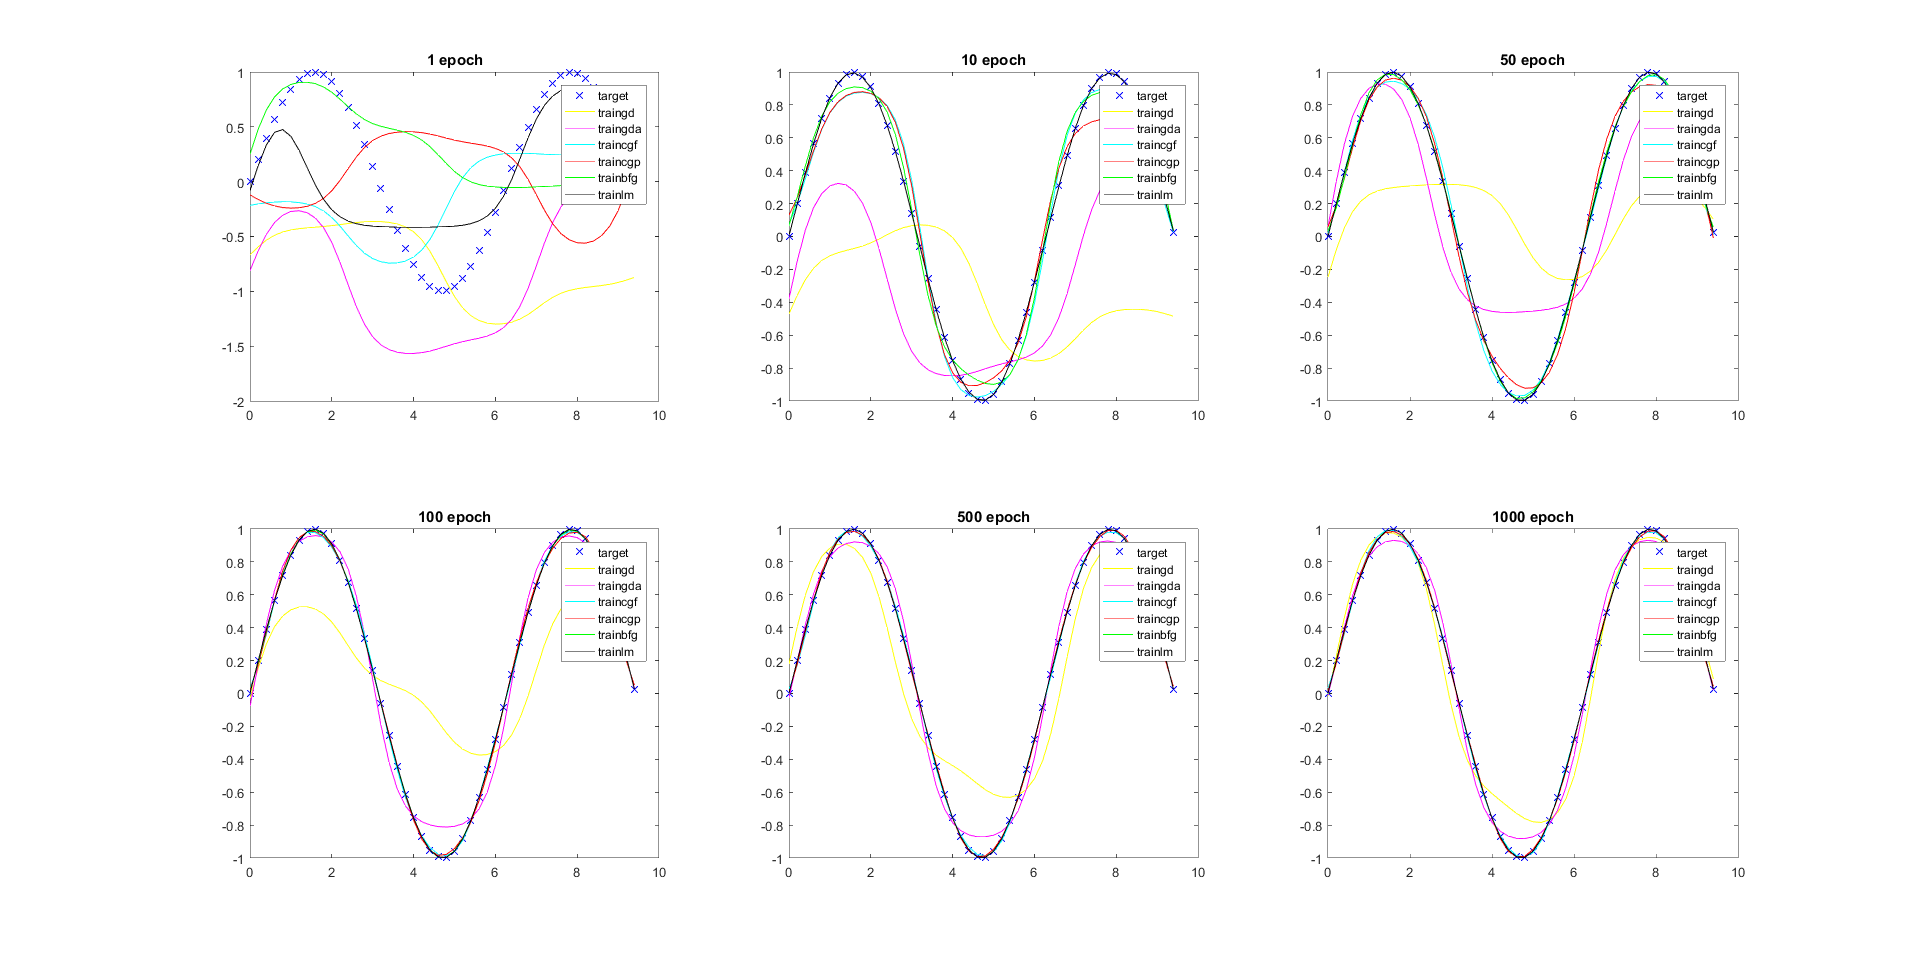
\includegraphics[width=\textwidth]{figures_1/pure_section2}
%\centering
%\end{figure}
\bigbreak
The results clearly indicate that \textit{Levenberg-Marquardt} algorithm (trainlm) converges quicker than the other learning algorithms. As we expected, \textit{Gradient descent} algorithm (traingd) is the slowest to converge. One interesting point in figure \ref{noisy_section2} is that \textit{trainlm} tends to overfit the curve, which illustrate that one should consider an early stop criteria before \textit{trainlm} starts to overfit in order to increase the generalization of the overall model.

\begin{figure}[!htbp]
\caption{Results of the FFNN prediction using different training algorithms in a noisy data.}
\label{noisy_section2}
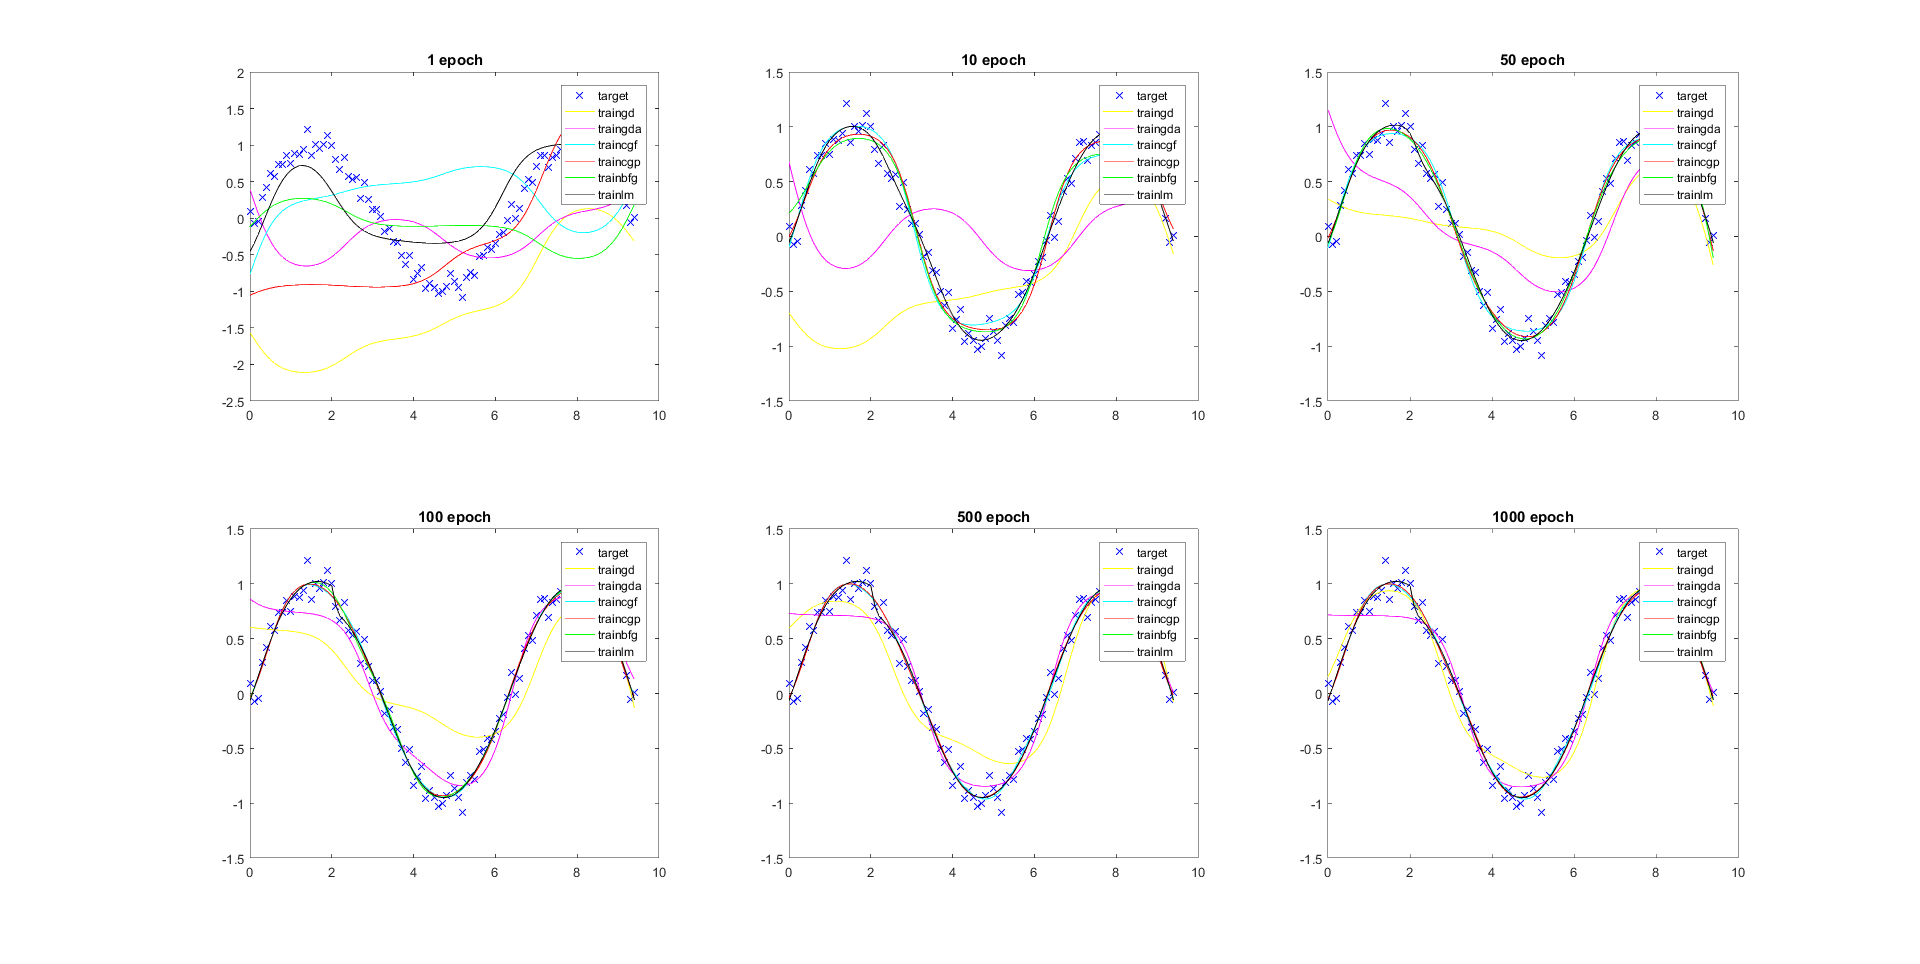
\includegraphics[width=\textwidth]{figures_1/noisy_section2}
\centering
\end{figure}


\subsection{Bayesian inference of networks hyperparameters}
\textit{Bayesian regularization backpropagation} algorithm (trainbr) was tested on a noisy data, similar to the previous section, as well as \textit{trainlm}. Different numbers of neurons were tested. Figures \ref{noisy_section24} and \ref{noisy_section25} show the extreme results of the experiments.
\bigbreak
It it is shown that, at the beginning of the learning phase,  \textit{trainbr} has a very bad model compared to \textit{trainlm}. However after a relatively small number of epochs \textit{trainbr} converges. According with the experiments, the speed rate to obtain a fairly good model from the \textit{trainbr} is pretty similar to \textit{trainlm}. The number of neurons in the hidden layer clearly affect both algorithms. The bigger the number of neurons has, the bigger the overfitting is; which implies that the generalization of the model is small. To conclude, a good trade-off between number of neurons and epochs must be set properly in order to have a good model with high generalization.
\begin{figure}[!htbp]
\caption{Results of the FFNN prediction using \textit{Bayesian regularization backpropagation} and \textit{Levenberg-Marquardt} algorithms in a noisy data using 5 neurons in the hidden layer.}
\label{noisy_section24}
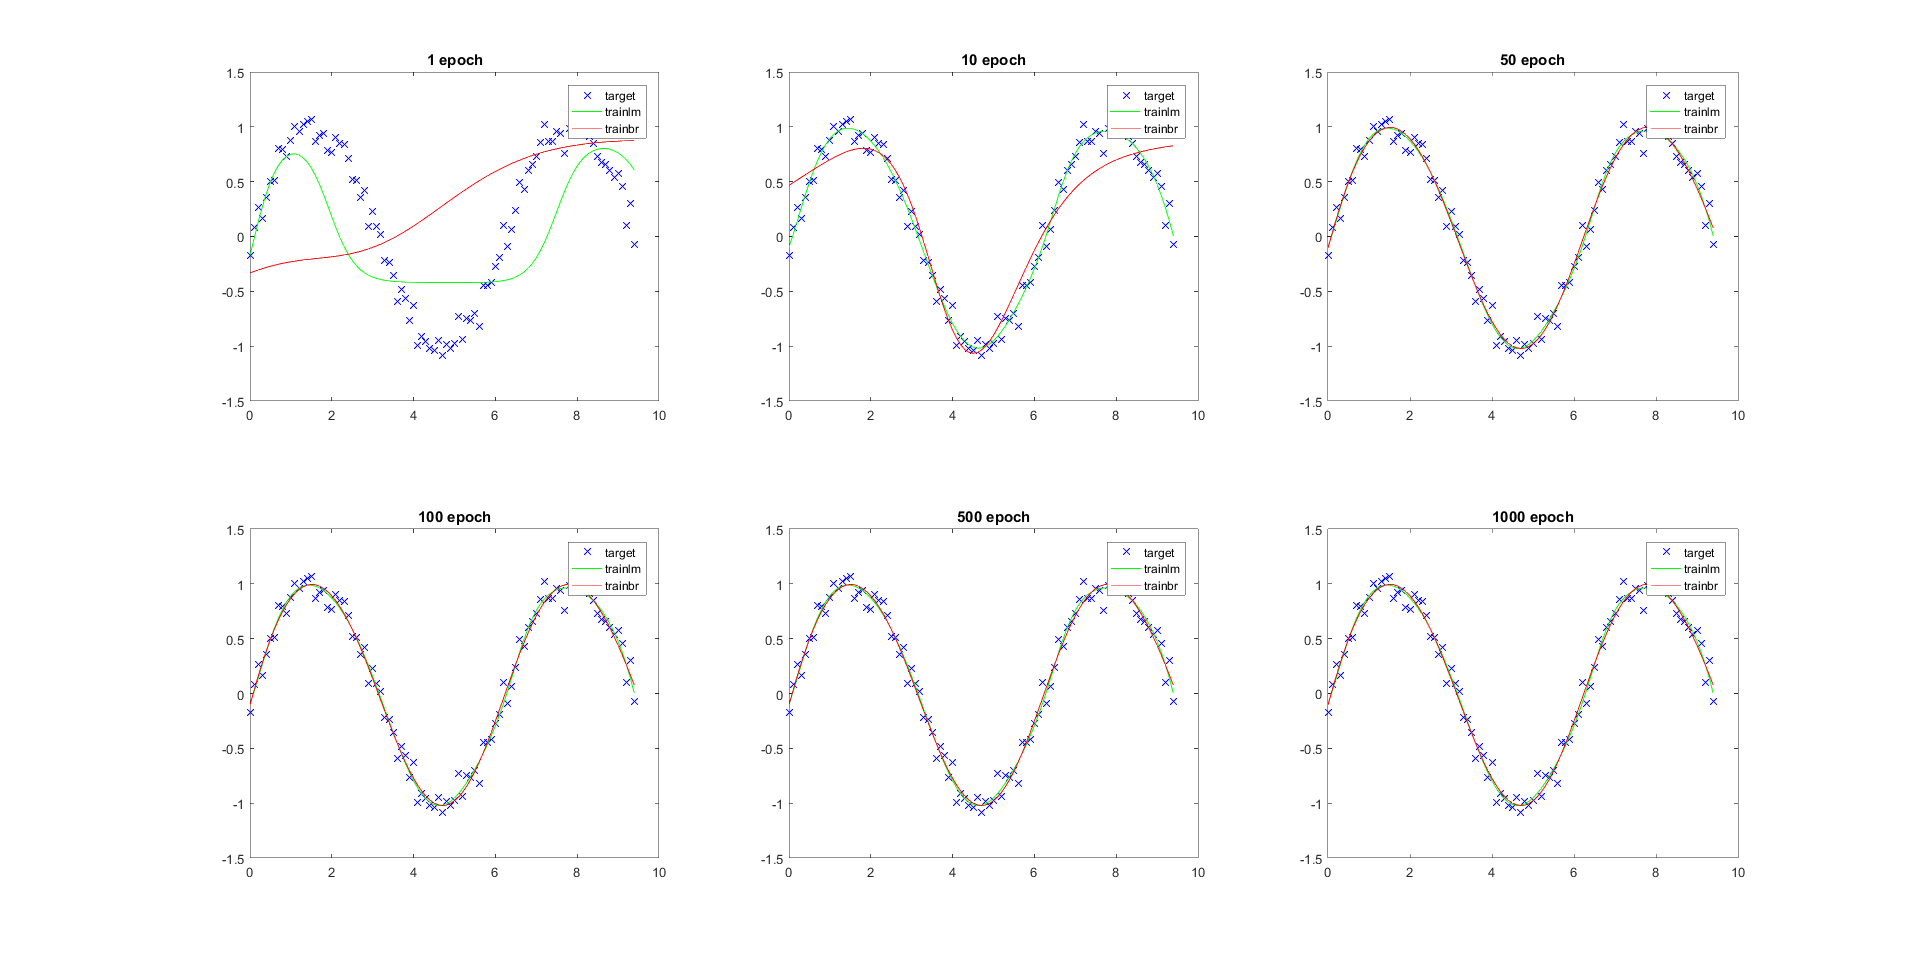
\includegraphics[width=\textwidth]{figures_1/noisy_section4_5n}
\centering
\end{figure}

\begin{figure}[!htbp]
\caption{Results of the FFNN prediction using \textit{Bayesian regularization backpropagation} and \textit{Levenberg-Marquardt} algorithms in a noisy data using 30 neurons in the hidden layer}
\label{noisy_section25}
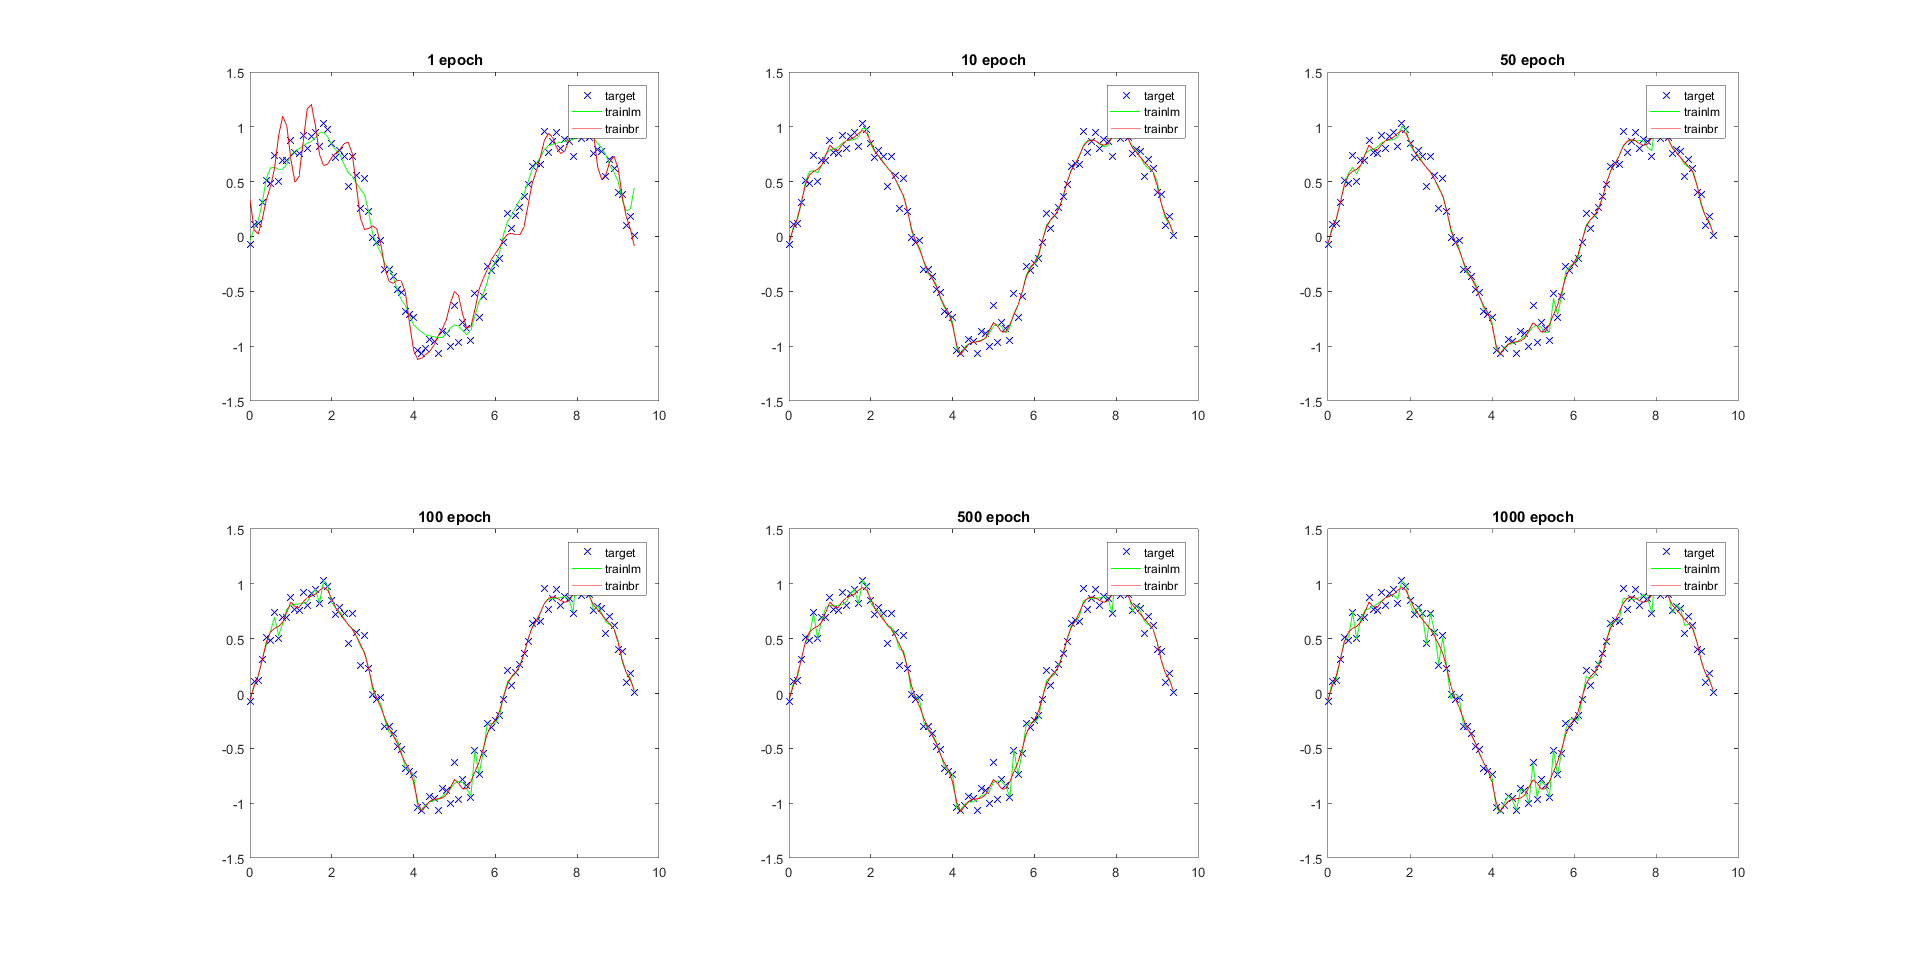
\includegraphics[width=\textwidth]{figures_1/noisy_section4_30n}
\centering
\end{figure}

\newpage
\section{S2: Recurrent neural networks}
\subsection{Hopfield networks}
Extreme cases of the noise parameter and number of iterations were tested on the \textit{hopdigit} example. Figures \ref{sec2_2} to \ref{sec2_3} show the results of 4 extreme experiments.
\bigbreak
Results in figures \ref{sec2_2} and \ref{sec2_4} show unstable states due to the limited number of iterations during the process. Hence the results did not converge. Nevertheless, the unstable states are relatively \textit{closed} to the stable states shown in figures \ref{sec2_1} and \ref{sec2_4}.
\bigbreak
Results in figures \ref{sec2_1} and \ref{sec2_3} after a bigger amount of iterations. It is clear that the noise (which implies the initial position of the input) affects the final result, a bigger noise (bigger distance from the target attractor) results in an unexpected result, as shown in figure \ref{sec2_3}.
\bigbreak
After an exhaustive iteration, no spurious states were found. 
\begin{figure}[!htbp]
\caption{Results of the \textit{hopdigit} function with noise=4 and numiter=10.}
\label{sec2_2}
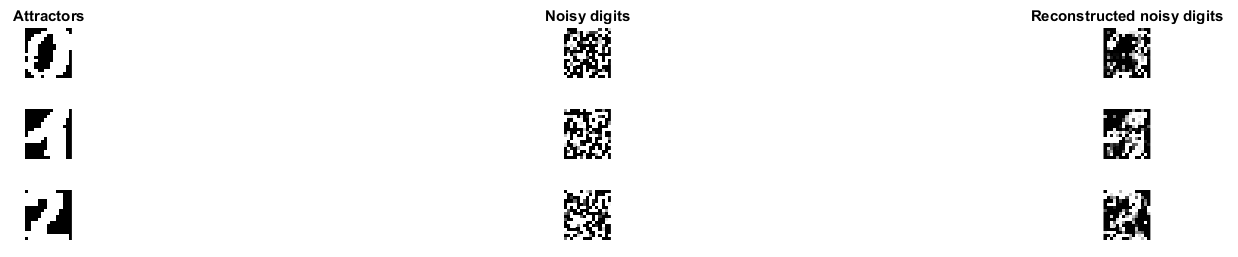
\includegraphics[width=\textwidth/2]{figures_2/hopdigit_4_10}
\centering
\end{figure}

\begin{figure}[!htbp]
\caption{Results of the \textit{hopdigit} function with noise=4 and numiter=100.}
\label{sec2_1}
\medbreak
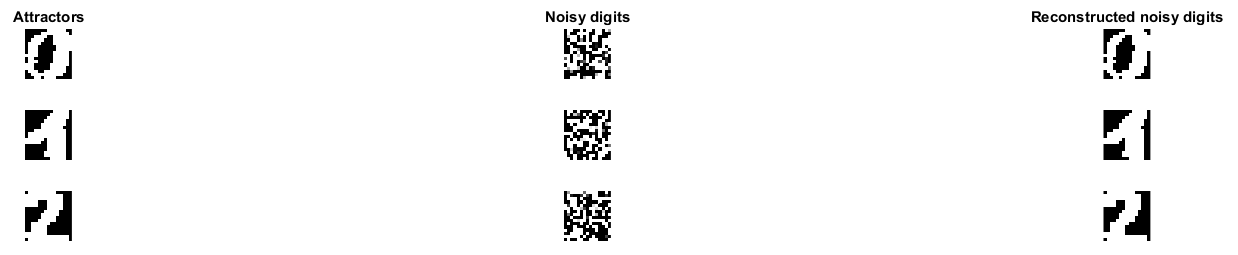
\includegraphics[width=\textwidth/2]{figures_2/hopdigit_4_1000_1}
\centering
\end{figure}

\begin{figure}[!htbp]
\caption{Results of the \textit{hopdigit} function with noise=100 and numiter=10.}
\label{sec2_4}
\medbreak
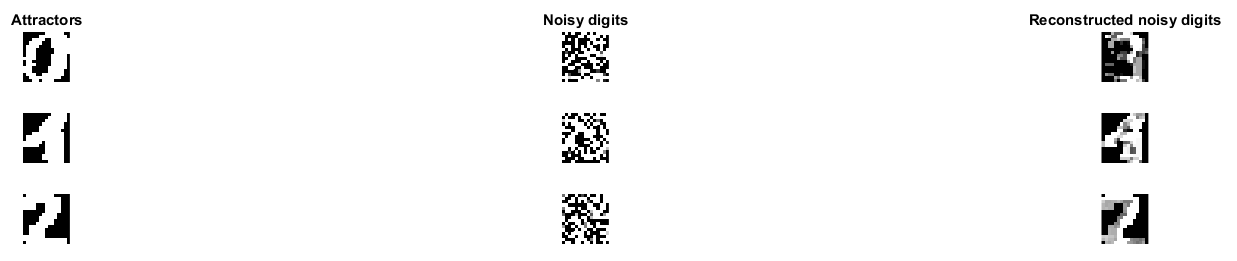
\includegraphics[width=\textwidth/2]{figures_2/hopdigit_10_10_1}
\centering
\end{figure}

\begin{figure}[!htbp]
\caption{Results of the \textit{hopdigit} function with noise=100 and numiter=100.}
\label{sec2_3}
\medbreak
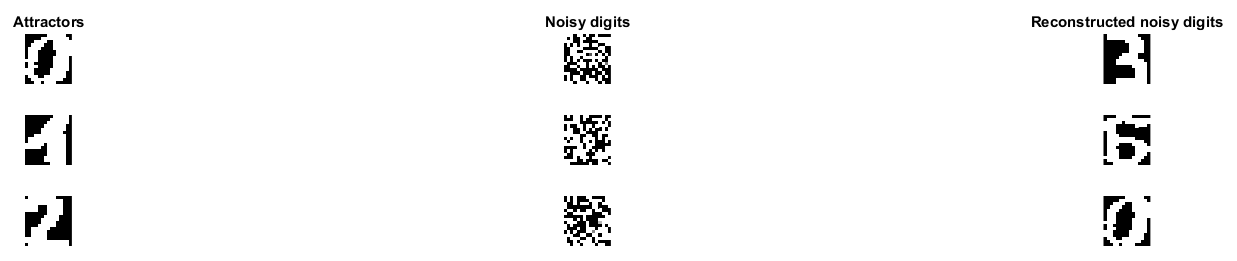
\includegraphics[width=\textwidth/2]{figures_2/hopdigit_100_100_2}
\centering
\end{figure}

\newpage

\subsection{Elman network}
Several experiments were done using different training points, epochs and neurons. To avoid a straightforward conclusion, three iterations per setup were run. Table \ref{s2_t1} shows the results.
\bigbreak
This experiments suggests that the number of neurons is a critical hyperparameter in the Helman network. There is a correlation between the recall and the neurons. There is a clearly negative effect when the number of neurons are increased. The number of epochs and training points increase the Recall and decrease the MSE in all the settings.


\begin{table}[!htbp]
\centering
\caption{Results of time-series predictions using an Elman network with different parameters}
\label{s2_t1}
\medbreak
\resizebox{\textwidth}{!}{
\begin{tabular}{c|c|c|c|c|c|c}
Training points & Epochs & Neurons & R1 - MSE1 & R2 - MSE2 & R3 - MSE3 & Avg R - Avg MSE \\\hline
300 & 100 & 50 & 0.8046 - 0.28165 & 0.86376 - 0.19918 & 0.82022 - 0.21337 & 0.82952 - 0.23140\\\hline
300 &  100 & 100 & 0.25316 - 0.74488 & 0.84409 - 0.22219 & 0.74083 - 0.24923 & 0.61269 - 0.40543\\\hline
300 &  100 & 500 & 0.066352 - 4.1895 & -0.37543 - 1.7456 & 0.36863 - 2.6571 & 0.01985 - 2.86406\\\hline

300 & 500 & 50 & 0.87958 - 0.17177 & 0.89757 - 0.14329 & 0.919663 - 0.13059 & 0.89893 - 0.44560\\\hline
300 &  500 & 100 & 0.83692 - 0.19721 & 0.77193 - 0.35833 & 0.8484 - 0.21193 & 0.81908 - 0.25582\\\hline
300 &  500 & 500 & 0.26619 - 2.4972 & 0.20328 - 2.8426 & 0.77812 - 0.33735 & 0.41586 - 1.89238\\\hline

300 & 1000 & 50 & 0.90988 - 0.1029 & 0.92109 - 0.089881 & 0.89314 - 0.14156 & 0.90803 - 0.11144\\\hline
300 & 1000 & 100 & 0.79292 - 0.34087 & 0.85052 - 0.23548 & 0.93913 - 0.095492 & 0.86085 - 0.22394\\\hline
300 & 1000 & 500 & 0.88905 - 0.13257 & 0.77324 - 0.2473 & 0.74208 - 0.37589 & 0.80145 - 0.25192\\\hline

500 & 100 & 50 & 0.91346 - 0.70402 & 0.89814 - 0.12147 & 0.86020 - 0.17218 & 0.89363 - 0.33255 \\\hline
500 &  100 & 100 & 0.31444 - 1.0704 & 0.73214 - 0.35368 & 0.75021 - 0.26852 & 0.59893 - 0.56346\\\hline
500 &  100 & 500 & 0.058904 - 4.2432 & 0.082859 - 2.4775 & -0.028816 - 1.9908 & 0.03764 - 2.9038\\\hline

500 & 500 & 50 & 0.66104 - 0.83886 & 0.77711 - 0.29763 & 0.82016 - 0.23519 & 0.75277 - 0.45722 \\\hline
500 &  500 & 100 & 0.88826 - 0.15023 & 0.7454 - 0.28408 & 0.8295 -0.24462 & 0.82105 - 0.22631 \\\hline
500 &  500 & 500 & 0.3947 - 2.0466 & 0.71847 - 0.30259 & 0.41324 - 2.136 & 0.50880 - 1.49506\\\hline

500 & 1000 & 50 & 0.96242 - 0.053706 & 0.94135 - 0.082144 & 0.8931 - 0.12993 & 0.93229 - 0.08859\\\hline
500 & 1000 & 100 & 0.81748 - 0.25344 & 0.89584 - 0.14696 & 0.82683 - 0.25421 & 0.84671 - 0.21820\\\hline
500 & 1000 & 500 & 0.54997 - 1.2887 & 0.88085 - 0.15332 & 0.9128 - 0.11874 & 0.78120 - 0.52015

\end{tabular}}
\end{table}

\newpage
\section{S3: Unsupervised learning: PCA and SOM}
\subsection{Principal Component Analysis}
The PCA algorithm was implemented using the Matlab functions provided in the exercise document. Figure \ref{3_333} shows the mean of the whole data set as well as the first element and its corresponding reconstructed vector using different k. Figures in \ref{eigenvqlues_plot} shows the eigenvalues of the components and the reconstruction error using different k values.
\bigbreak
Comparing figures in \ref{eigenvqlues_plot}, there exists a relation between the reconstruction error and the eigenvalues. This implies that the number of k components directly influence the quality of the reconstruction. This can be verified on figure  \ref{3_333}, the reconstructed image from k=1 to k=2 clearly shows an aggresive improvement.

\begin{figure}[!htbp]
\caption{Left: Image of the mean vector of the whole data set. Right: Image of the first element of the dataset with different reconstructions.}
\label{3_333}
\medbreak
\begin{tabular}{ccccccc}
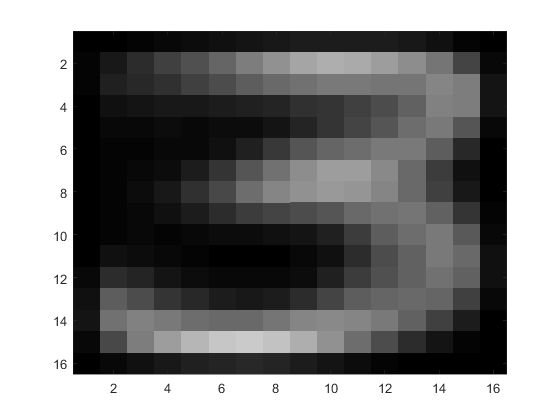
\includegraphics[width=\textwidth/7]{figures_3/mean_3} &
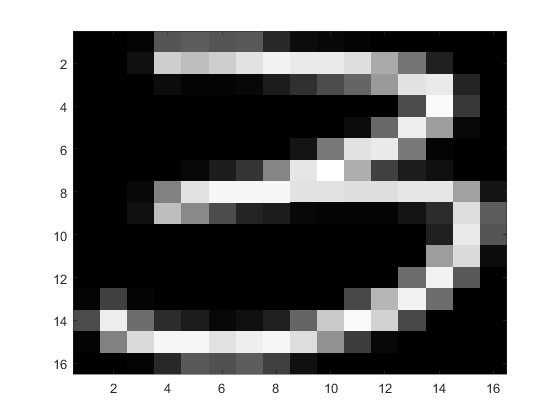
\includegraphics[width=\textwidth/7]{figures_3/k_0_1e} &
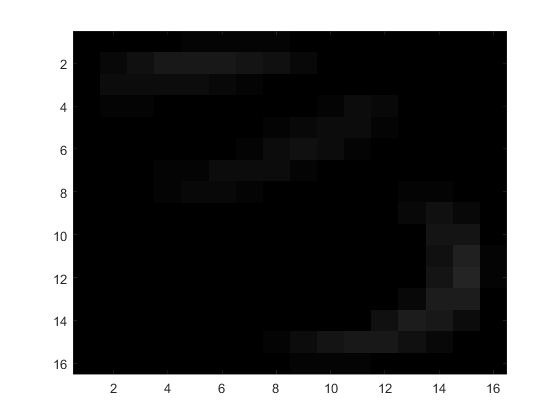
\includegraphics[width=\textwidth/7]{figures_3/k_1_1e} &
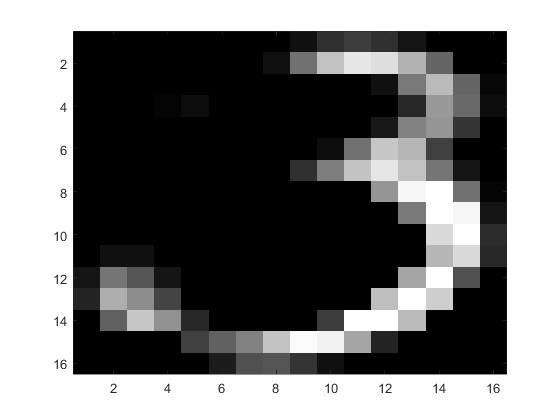
\includegraphics[width=\textwidth/7]{figures_3/k_2_1e} &
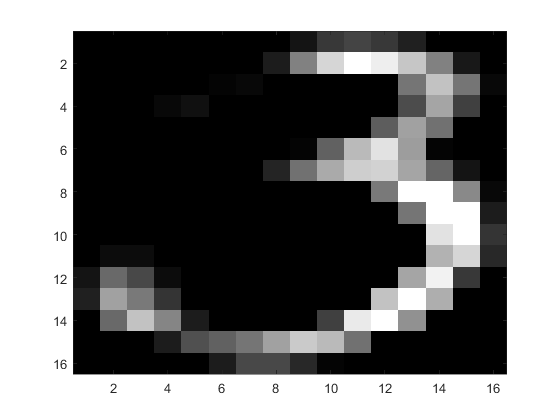
\includegraphics[width=\textwidth/7]{figures_3/k_3_1e} &
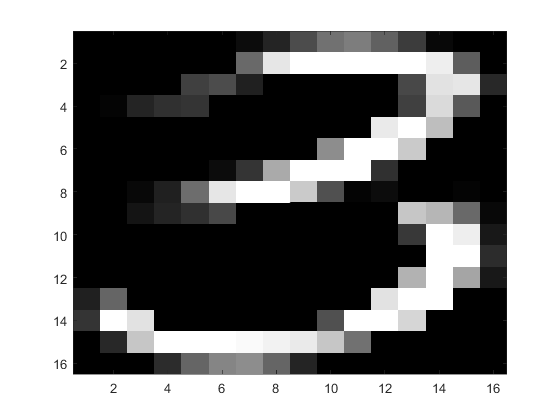
\includegraphics[width=\textwidth/7]{figures_3/k_4_1e}\\
 Mean & Original & k=1 & k=2 & k=3 & k=4\\
\end{tabular}
\centering
\end{figure}


\begin{figure}[!htbp]
\caption{Plots of PCA exercise.}
\label{eigenvqlues_plot}
  \centering
  \label{eigenvqlues_plot}
  \subfloat[Plot of the eigenvalues of the US Postal Service dataset. Axis X represents the \textit{i}th eigenvalue. Axis Y represents the eigenvalues.]{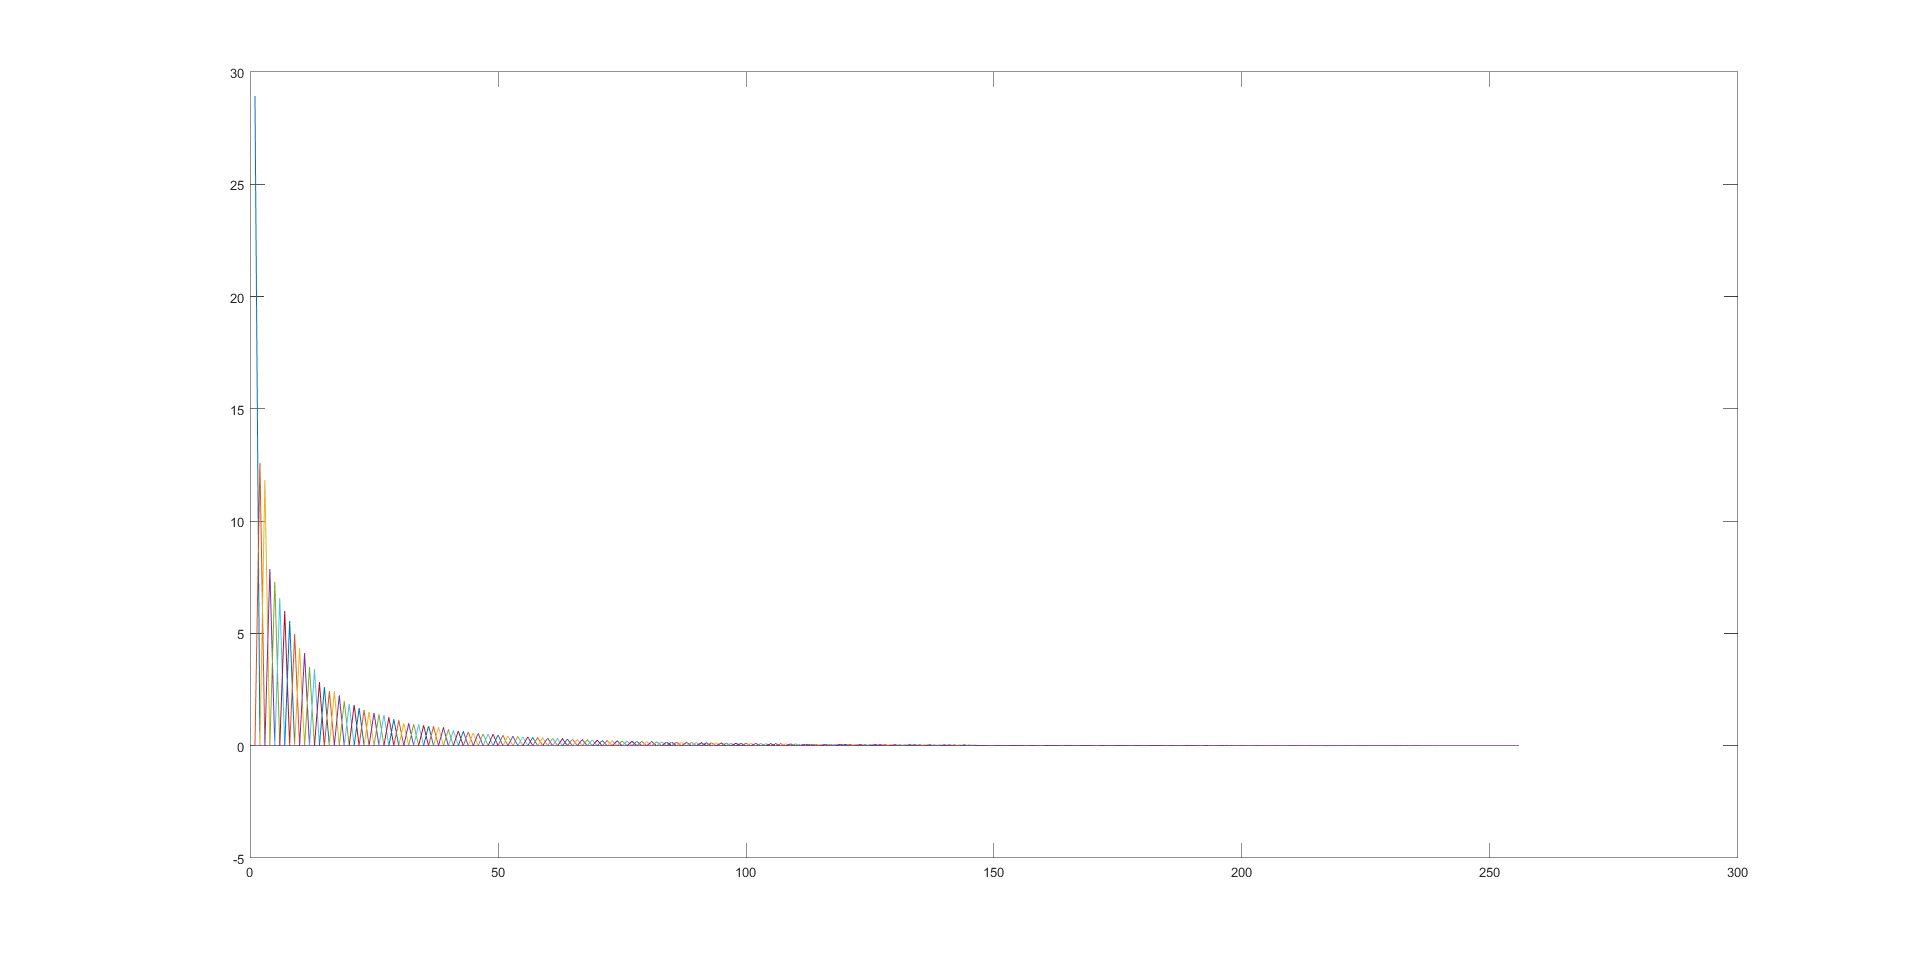
\includegraphics[width=0.4\textwidth]{figures_3/eigenvqlues_plot}\label{fig:f1}}
  \hfill
  \subfloat[Plot of the reconstructions error (MSE) from k=1 to k=256]{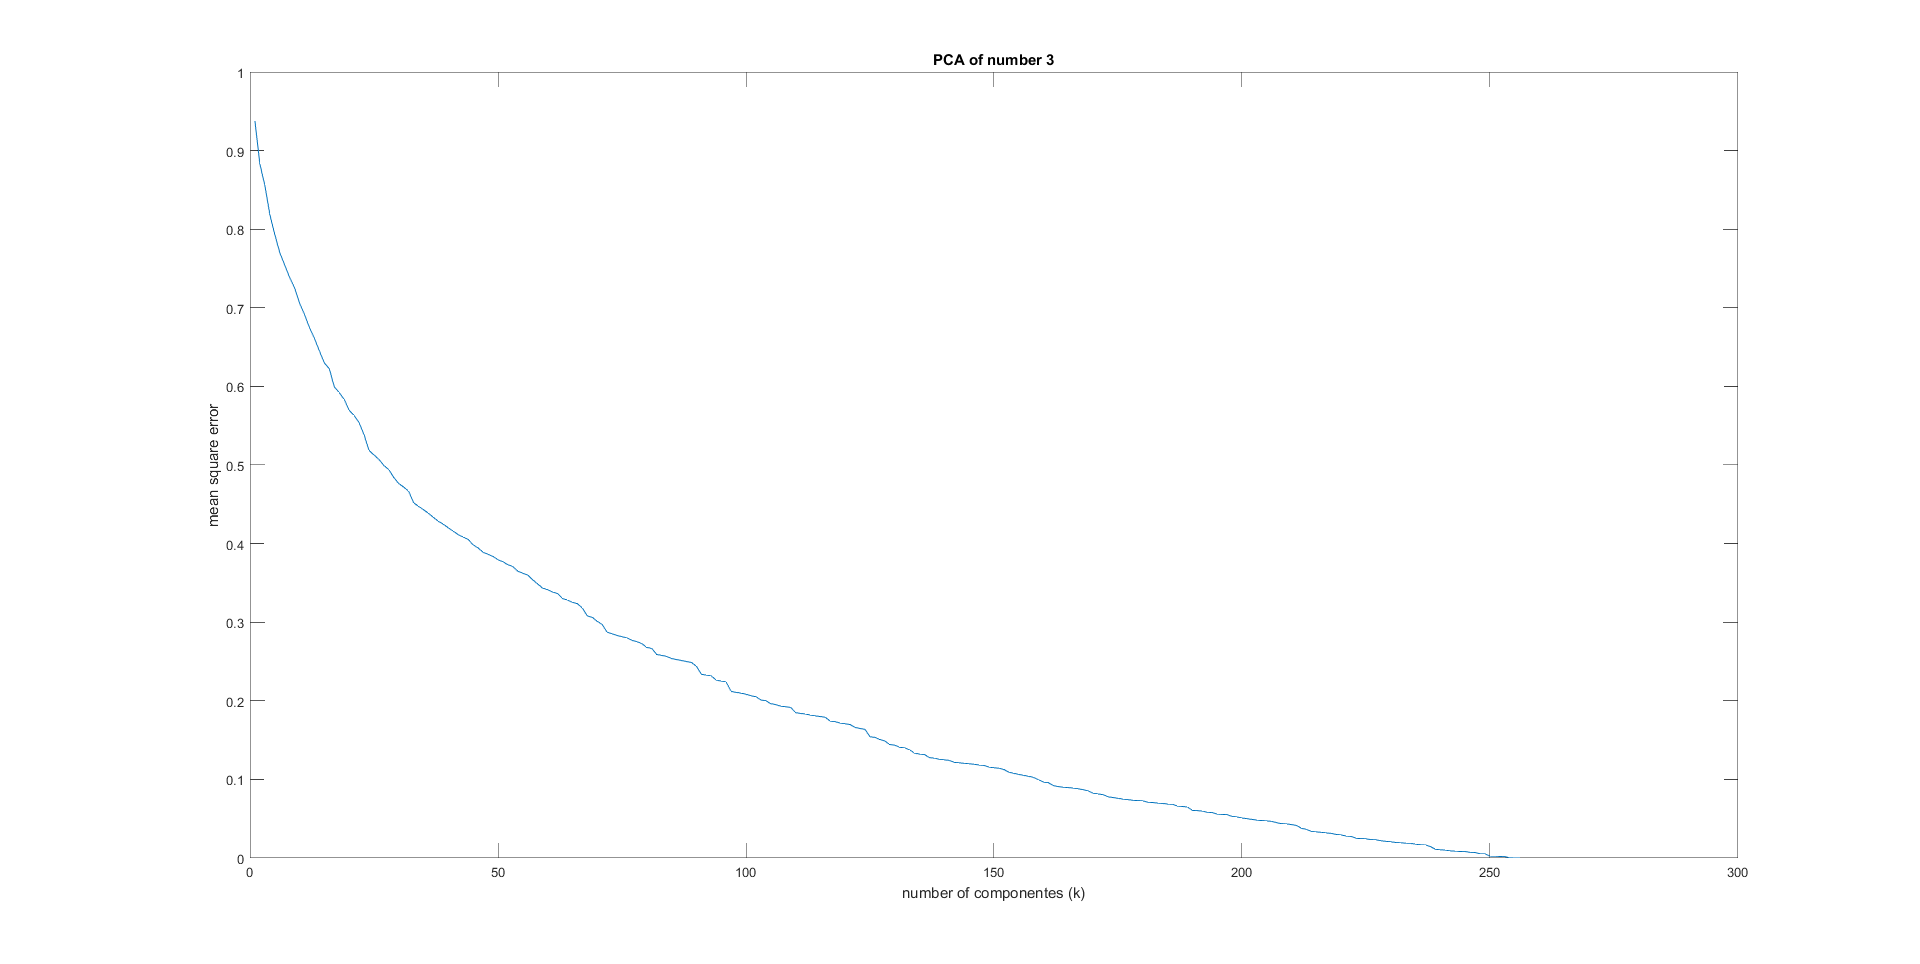
\includegraphics[width=0.4\textwidth]{figures_3/plot_k}\label{fig:f2}}
\end{figure}


\subsection{Competitive learning with SOM's}
Figure \ref{som_cylinder} shows the results of different experiment in \textbf{SOM\_concentric\_cylinders.m} script. The model used a hexagonal topology with a grid size of 5x5x5. \textit{Link distance} (linkdist) and \textit{Manhattan distance} (mandist) were tested with different epochs. 
\bigbreak
It is concluded that the \textit{linkdist} simulates a better cylinder shape (making it a heavily connected graph) than the \textit{mandist}.
\bigbreak
Figure \ref{panel_22} shows some results of different experiment in \textbf{example\_SOM\_iris.m} script. The model used different topologies and grid size of 10x10. \textit{Link distance} (linkdist) and \textit{Manhattan distance} (mandist) were tested with equal amount of epochs (100).
\bigbreak
A remark conclusion is that hexagonal topology shows a smoother topology than the grid topology. Additionally \textit{linkdist} gives harder limits on the decision surface than \textit{mandist} as shown in figure \ref{panel_22}.
\begin{figure}[!htbp]
\caption{Top: Trajectory of the neurons using Manhattan distance. Bottom: Trajectory of the neurons using Link distance.}
\label{som_cylinder}
\medbreak
\begin{tabular}{cccc}
 Initial state & epochs=10 & epochs=100 & epochs=1000\\\hline
 
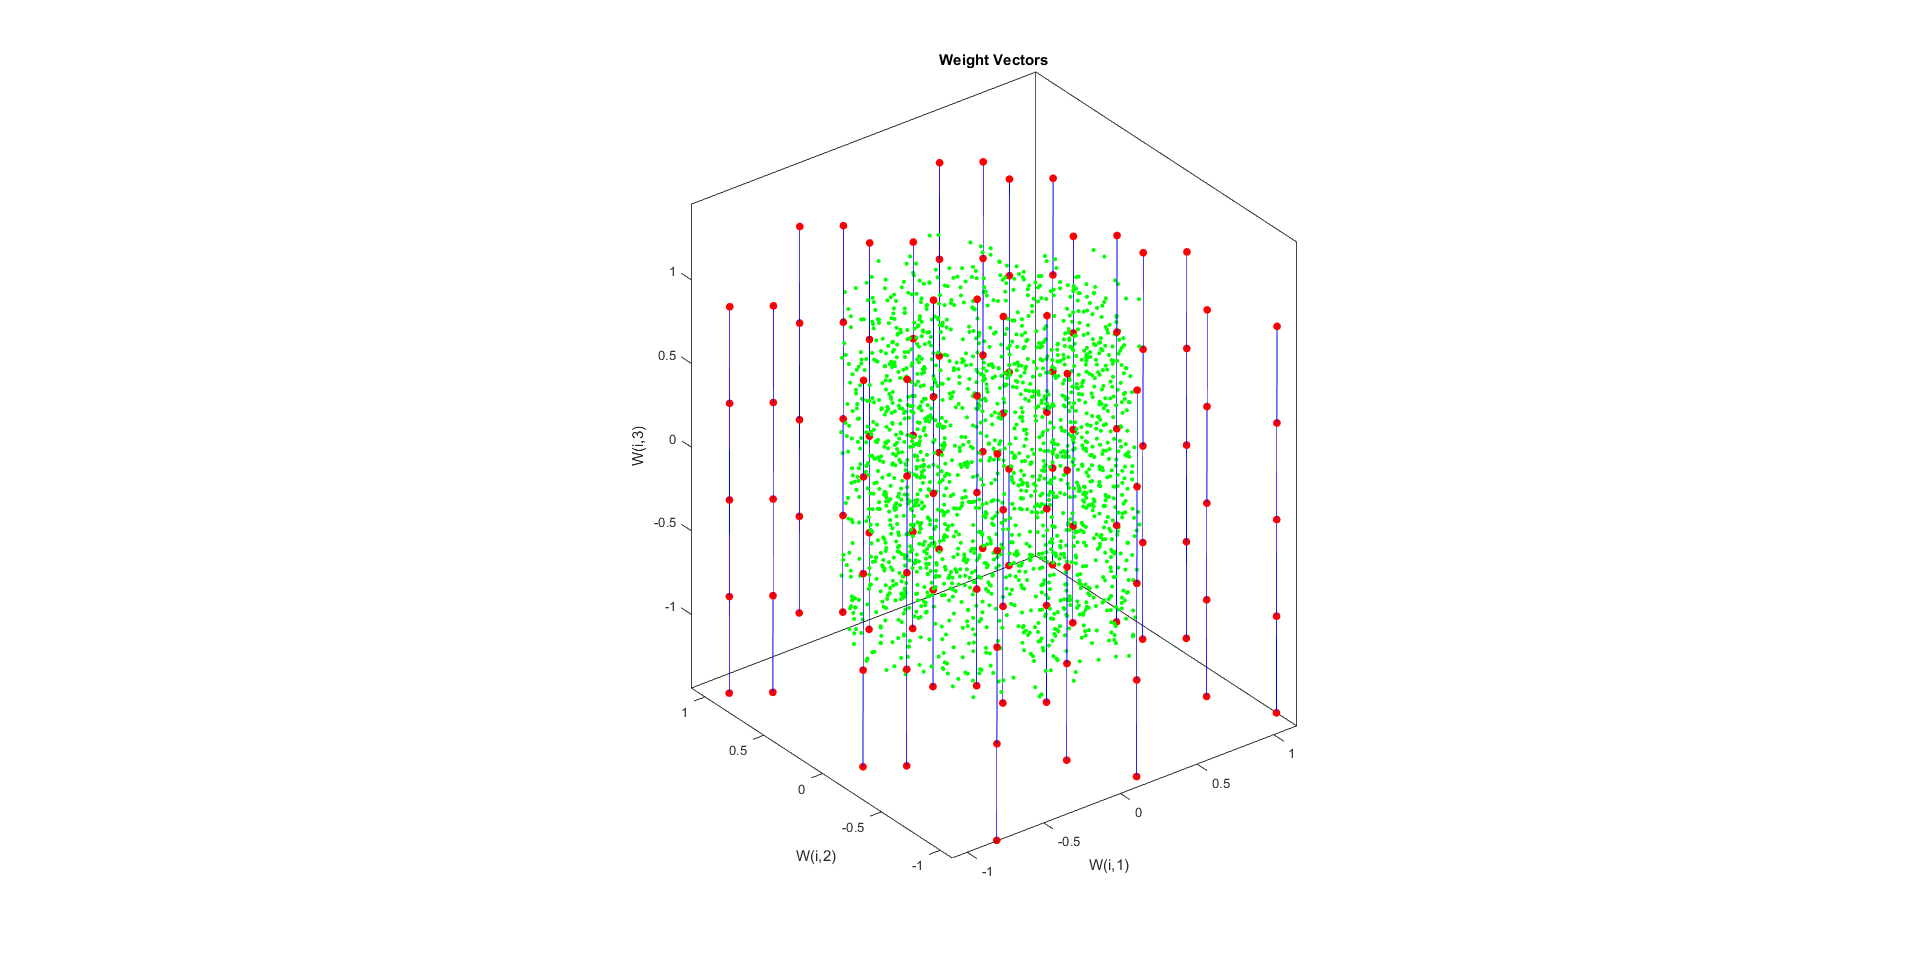
\includegraphics[width=\textwidth/5]{figures_3/som_0_1_mandist} &
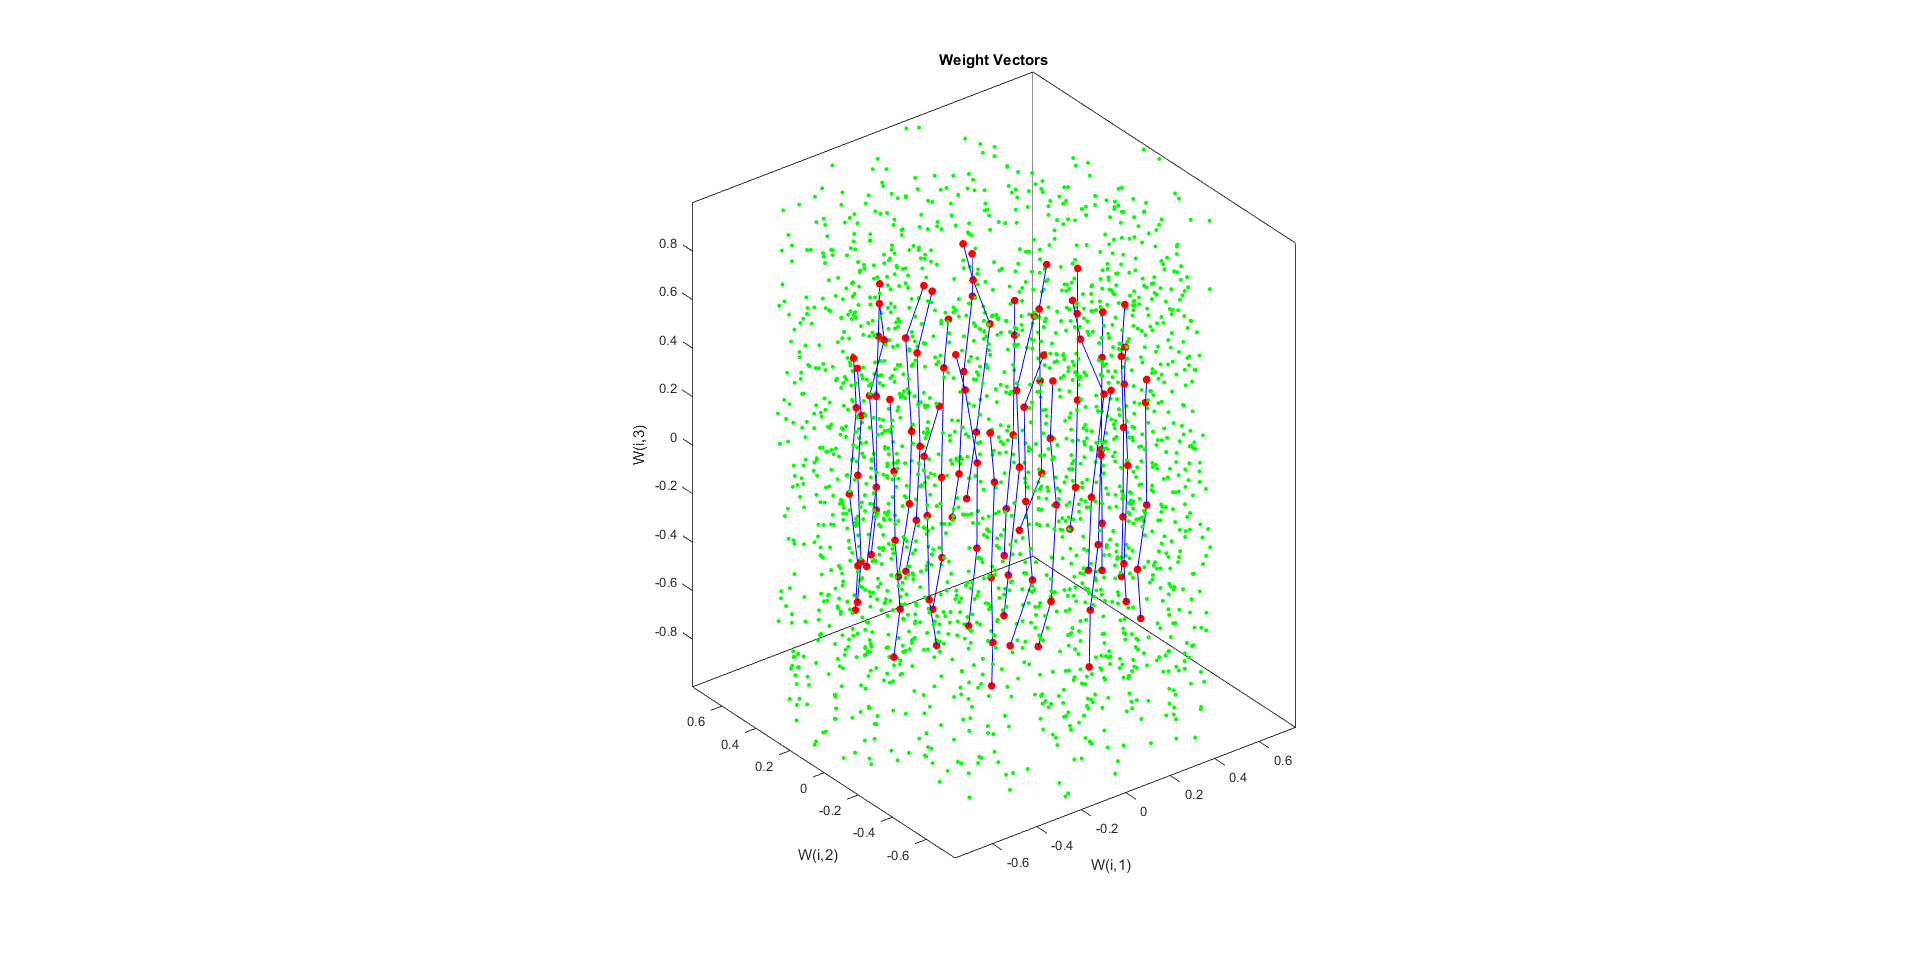
\includegraphics[width=\textwidth/5]{figures_3/som_10_1_mandist} &
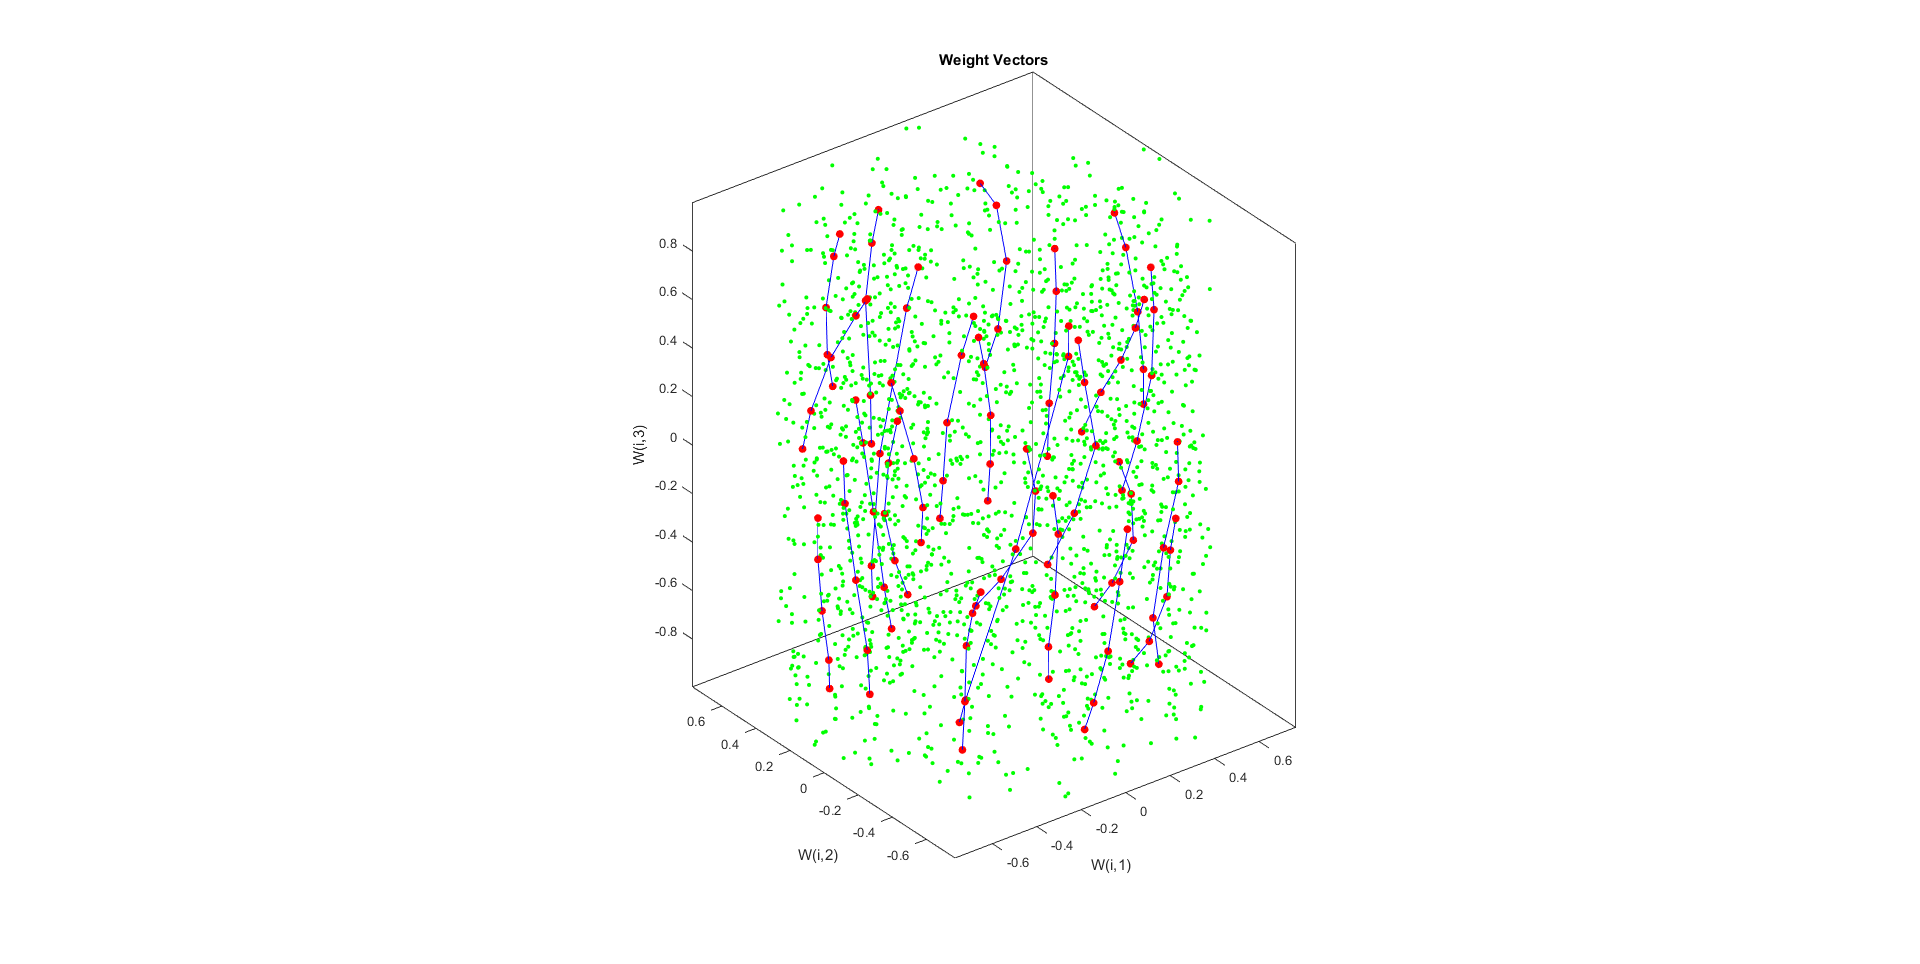
\includegraphics[width=\textwidth/5]{figures_3/som_100_1_mandist} &
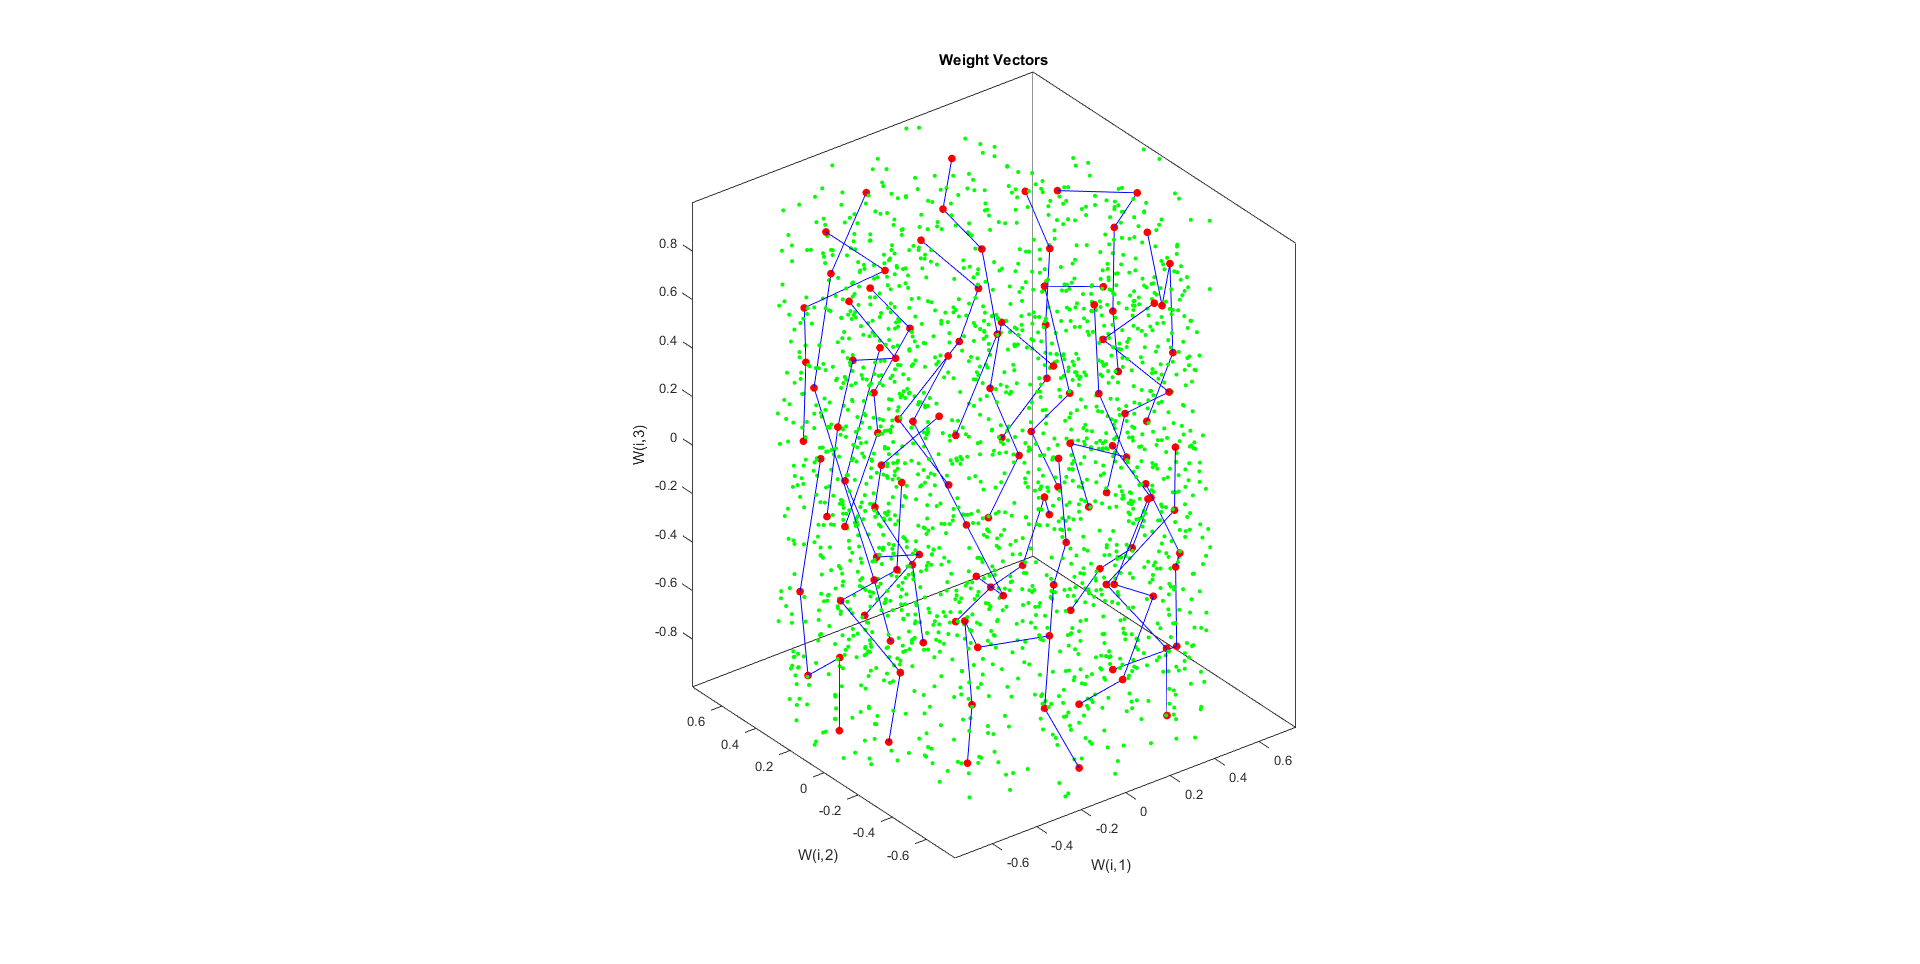
\includegraphics[width=\textwidth/5]{figures_3/som_1000_1_mandist} \\
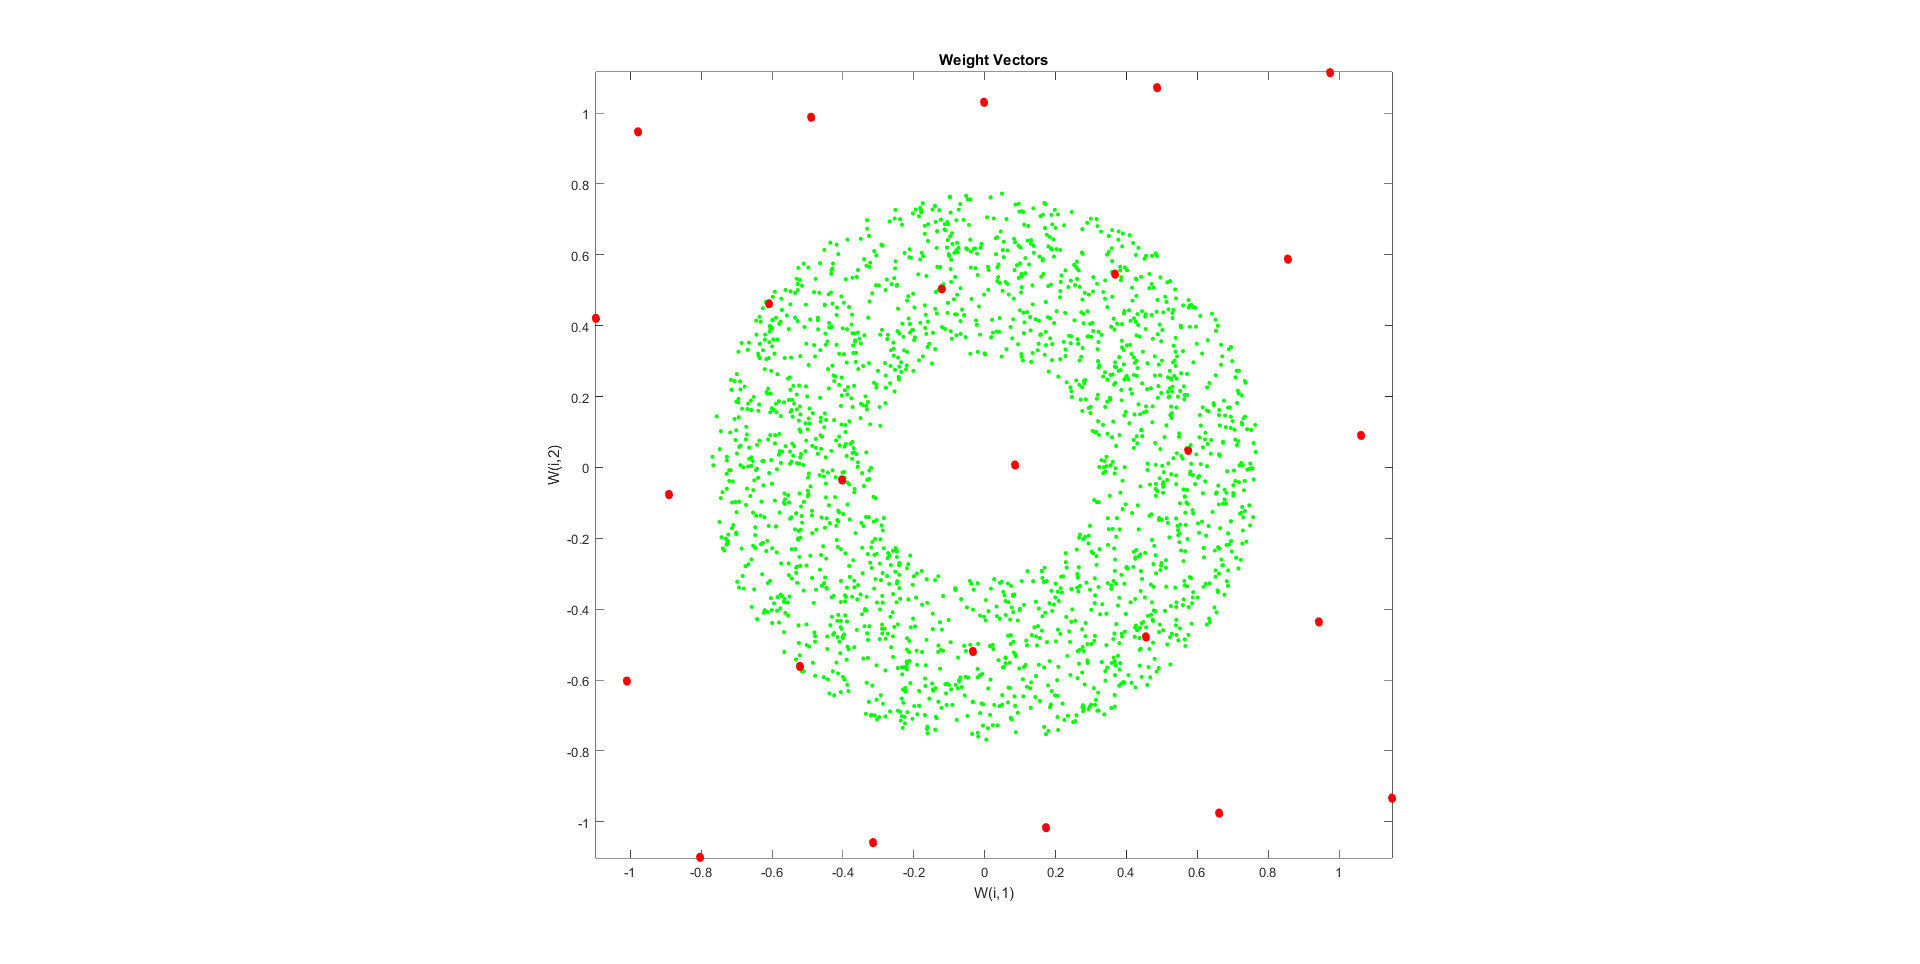
\includegraphics[width=\textwidth/5]{figures_3/som_0_2_mandist} &
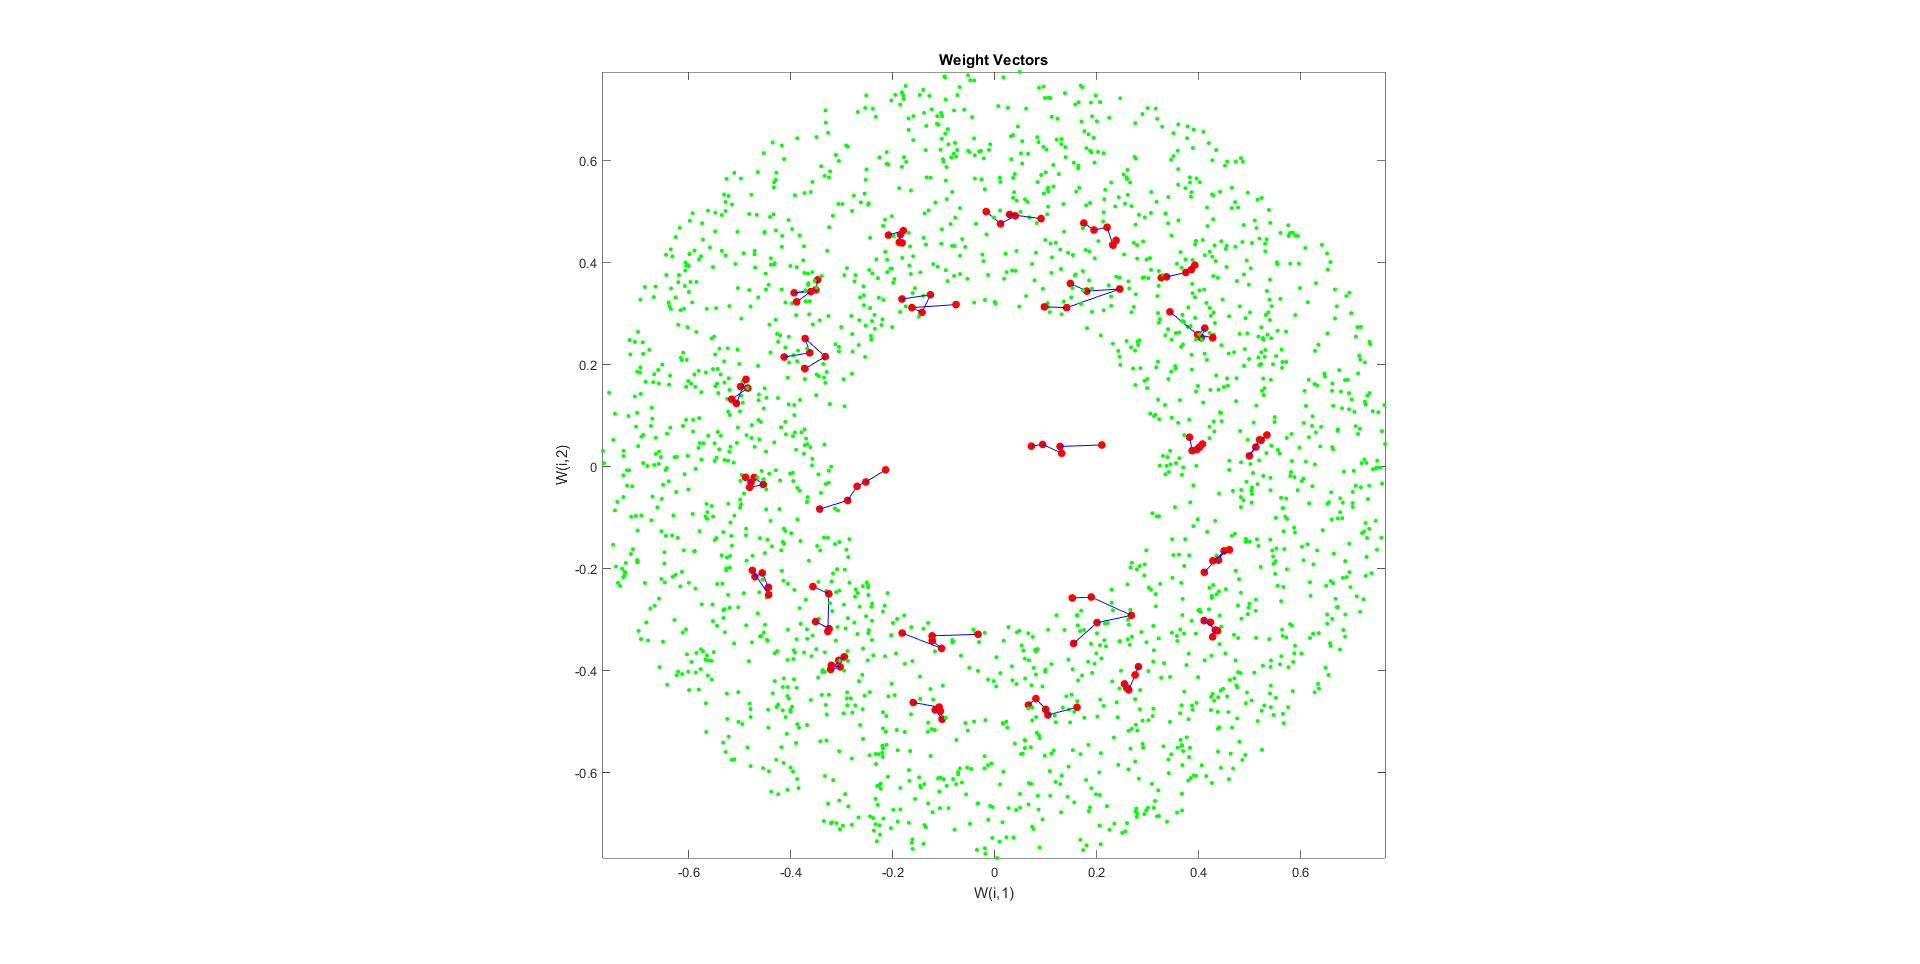
\includegraphics[width=\textwidth/5]{figures_3/som_10_2_mandist} &
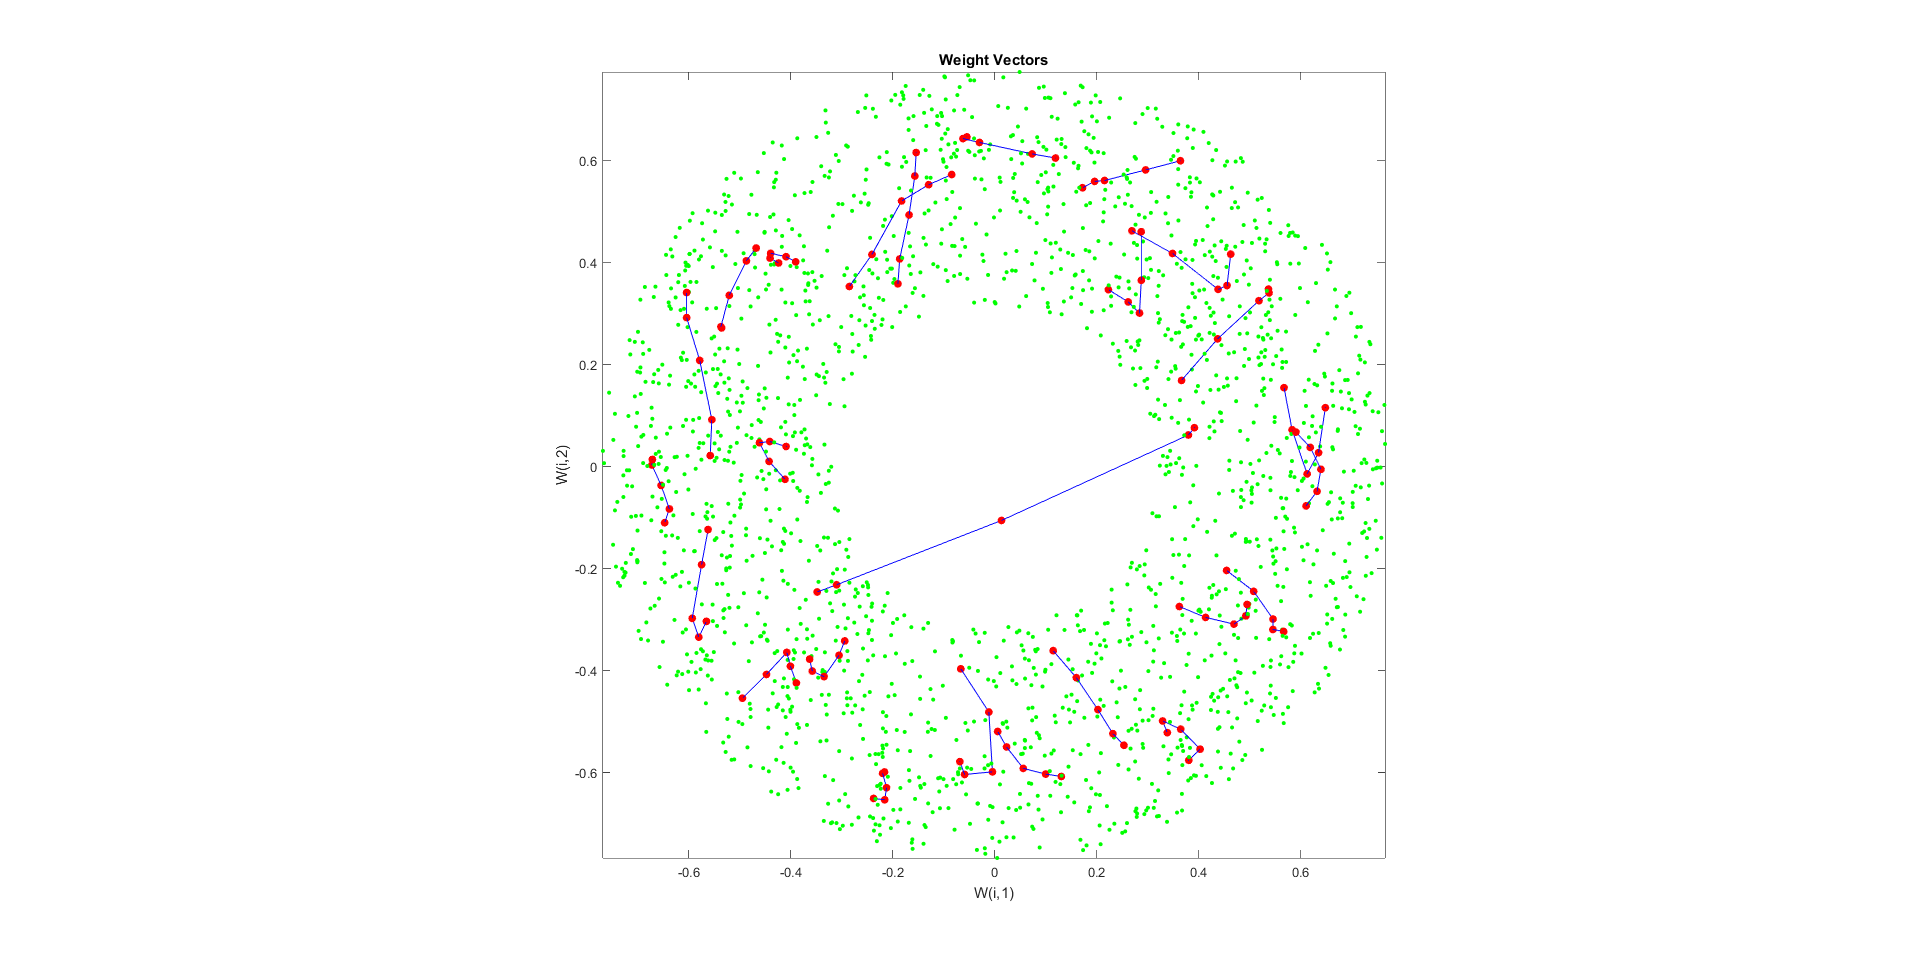
\includegraphics[width=\textwidth/5]{figures_3/som_100_2_mandist} &
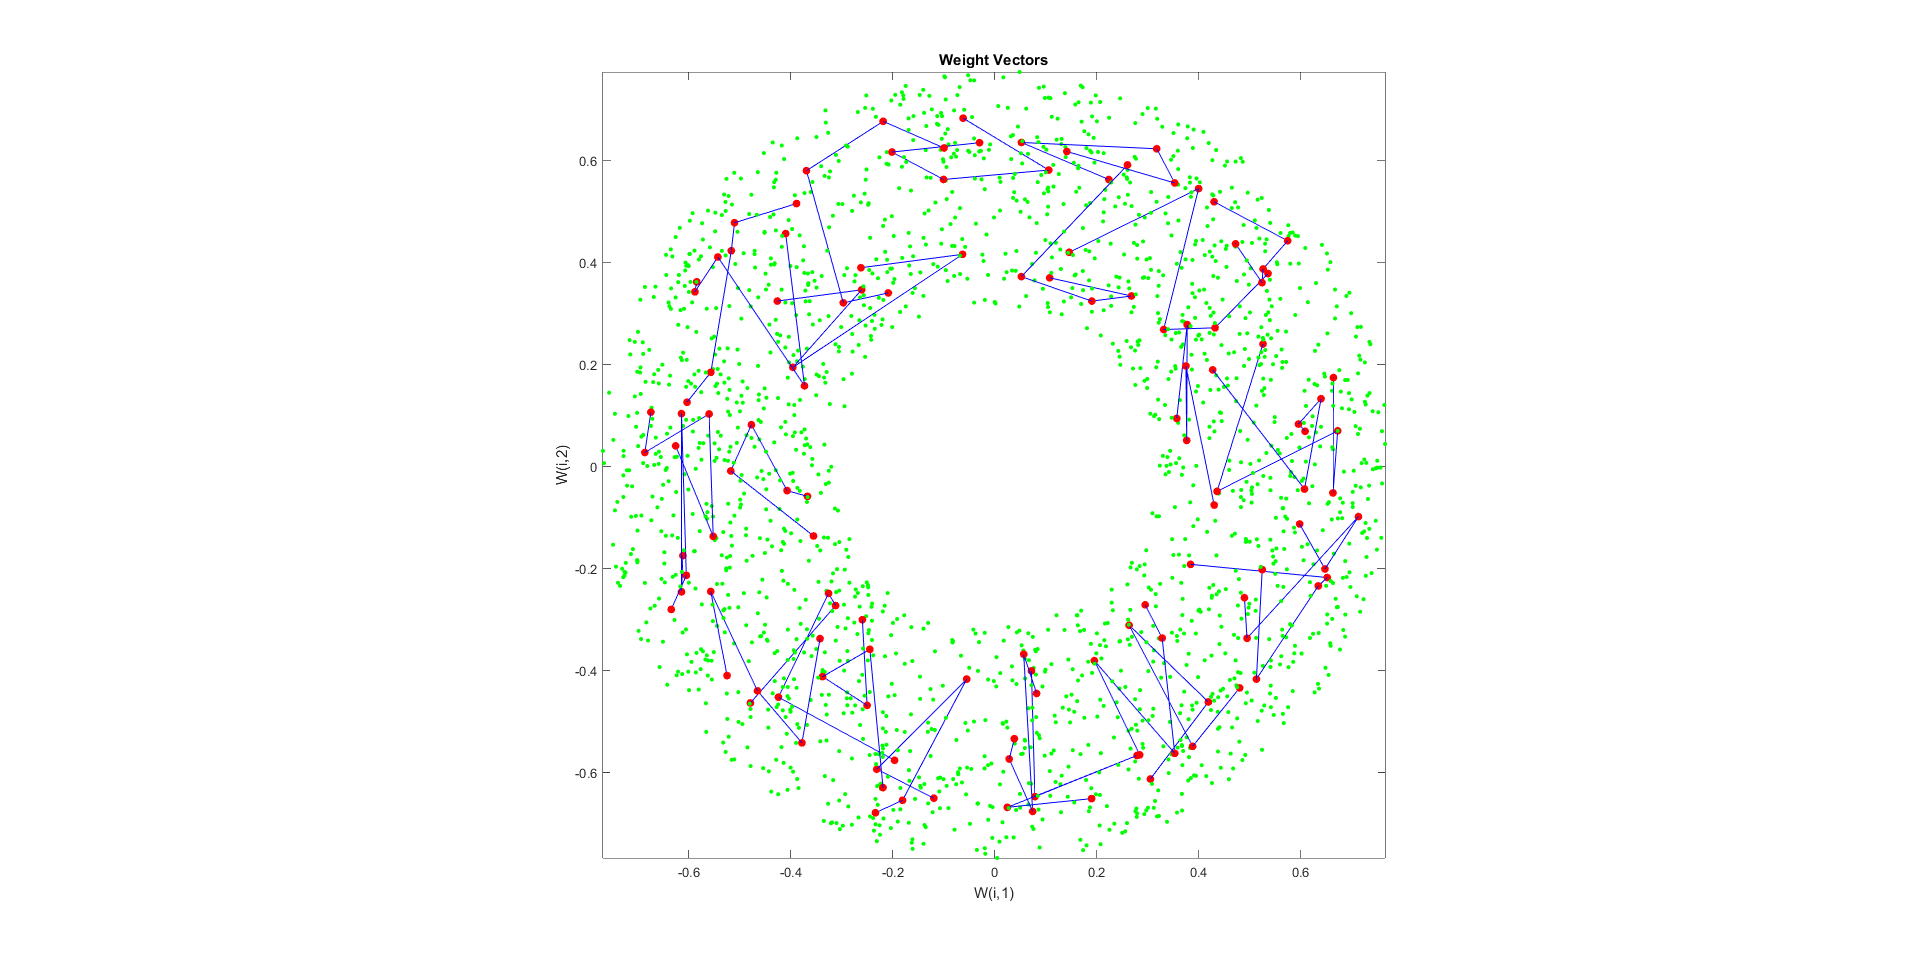
\includegraphics[width=\textwidth/5]{figures_3/som_1000_2_mandist} \\\hline

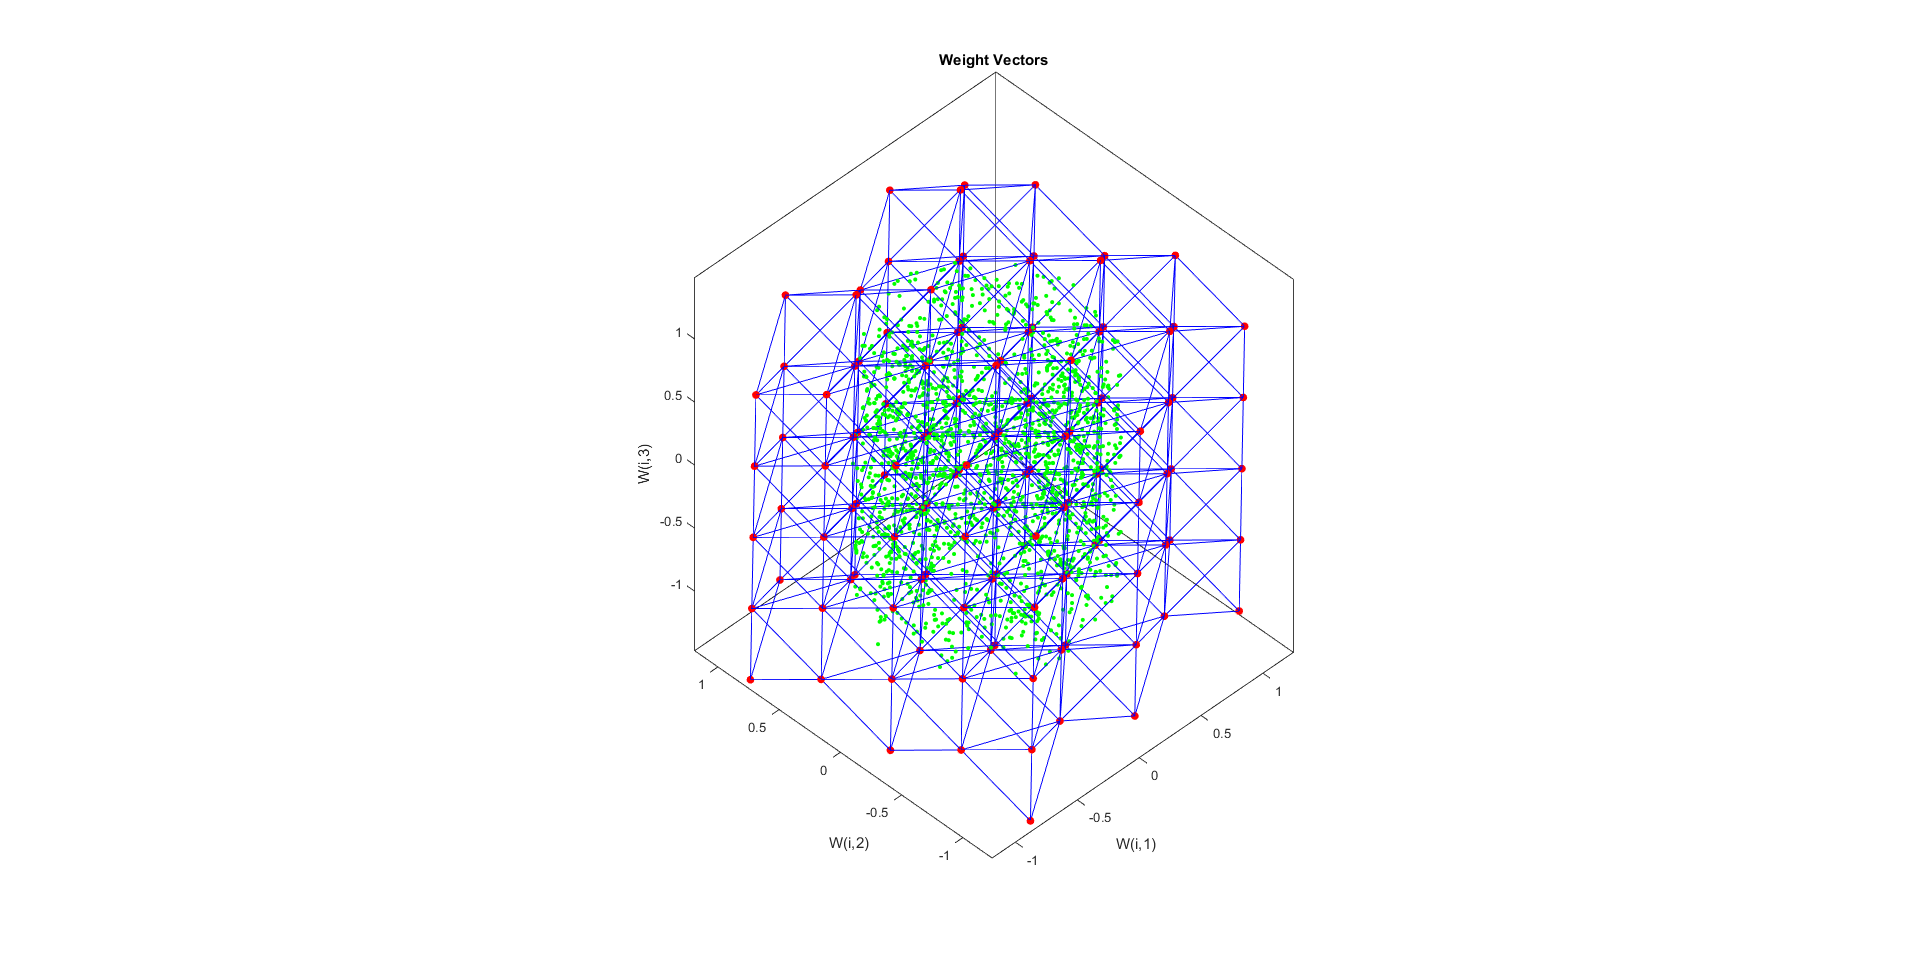
\includegraphics[width=\textwidth/5]{figures_3/som_0_1} &
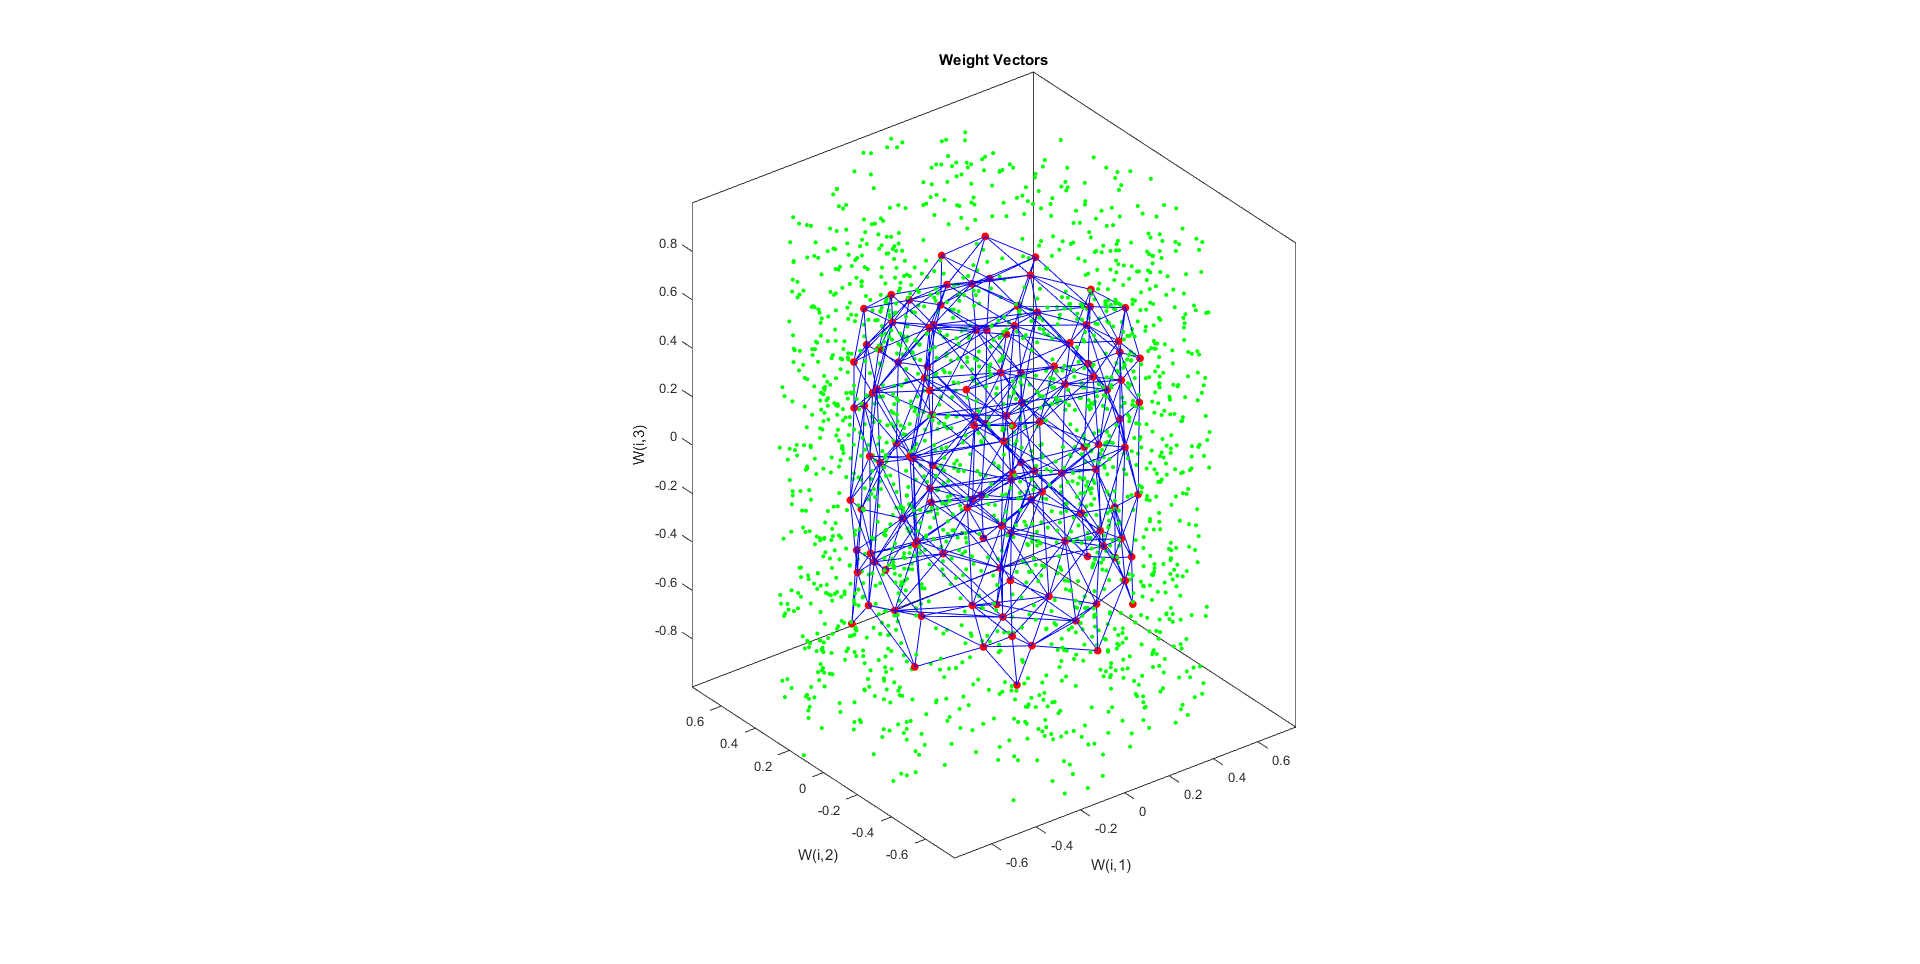
\includegraphics[width=\textwidth/5]{figures_3/som_10_1} &
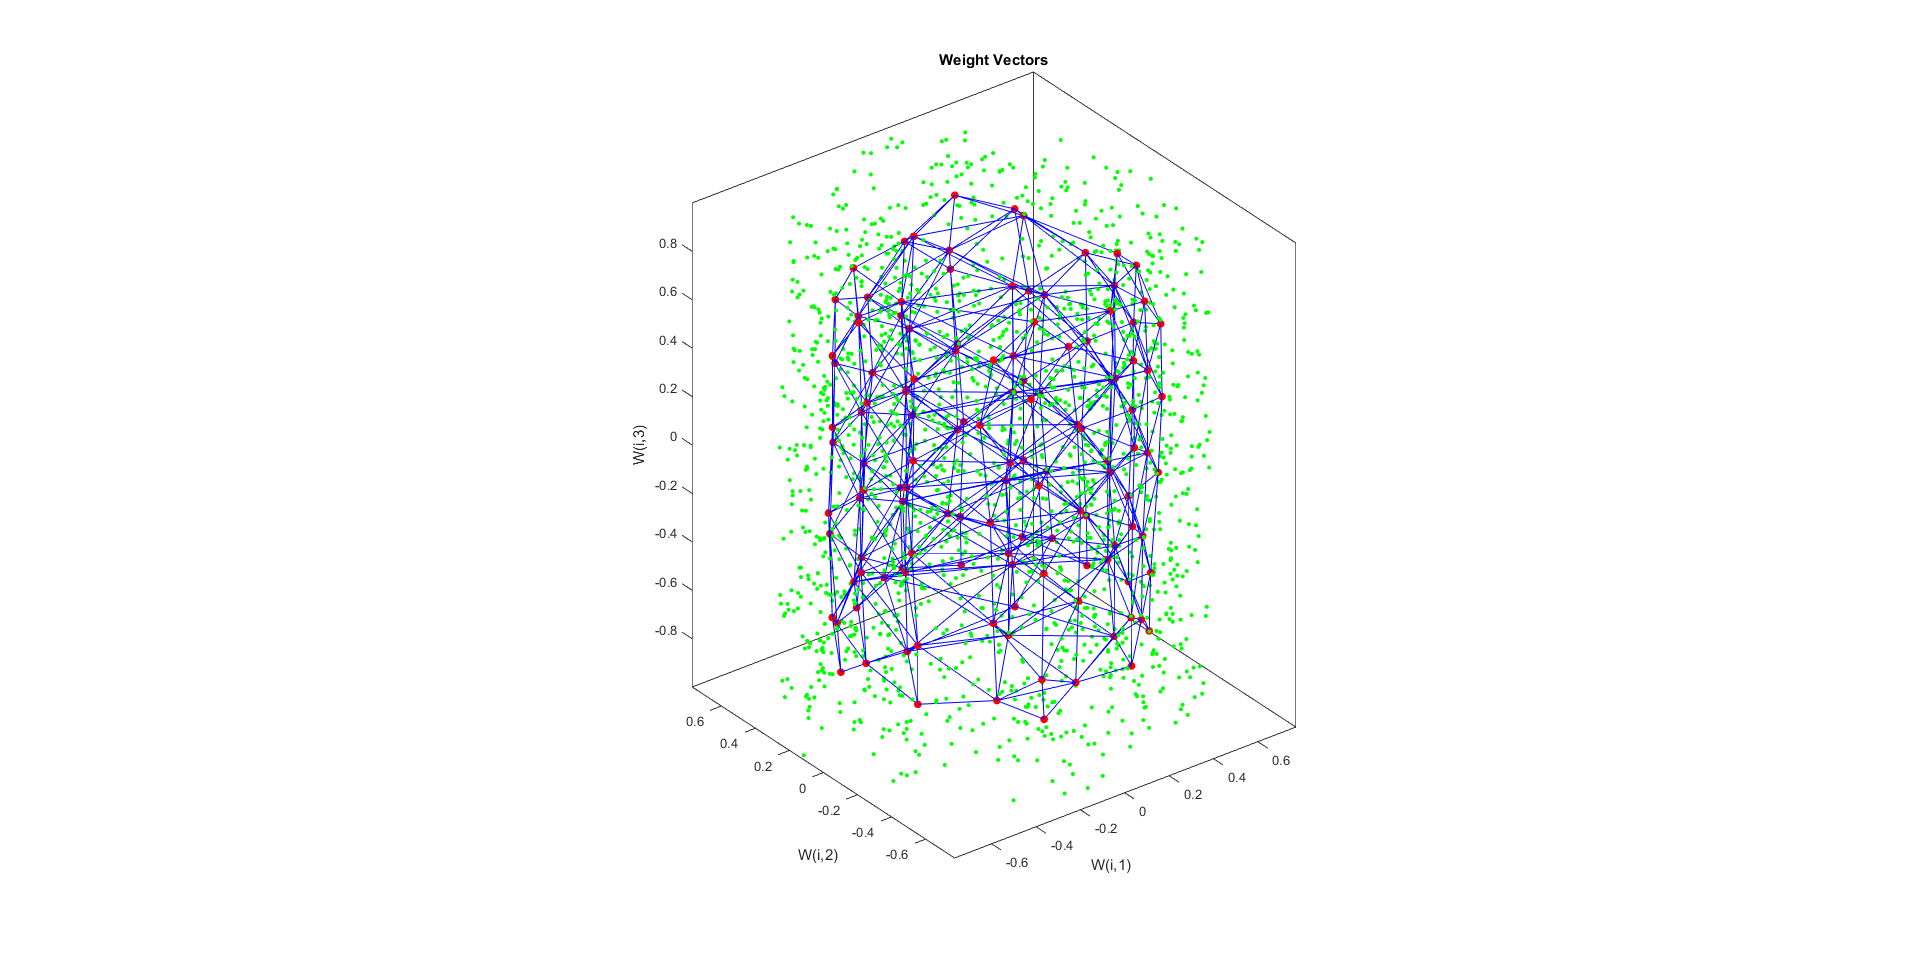
\includegraphics[width=\textwidth/5]{figures_3/som_100_1} &
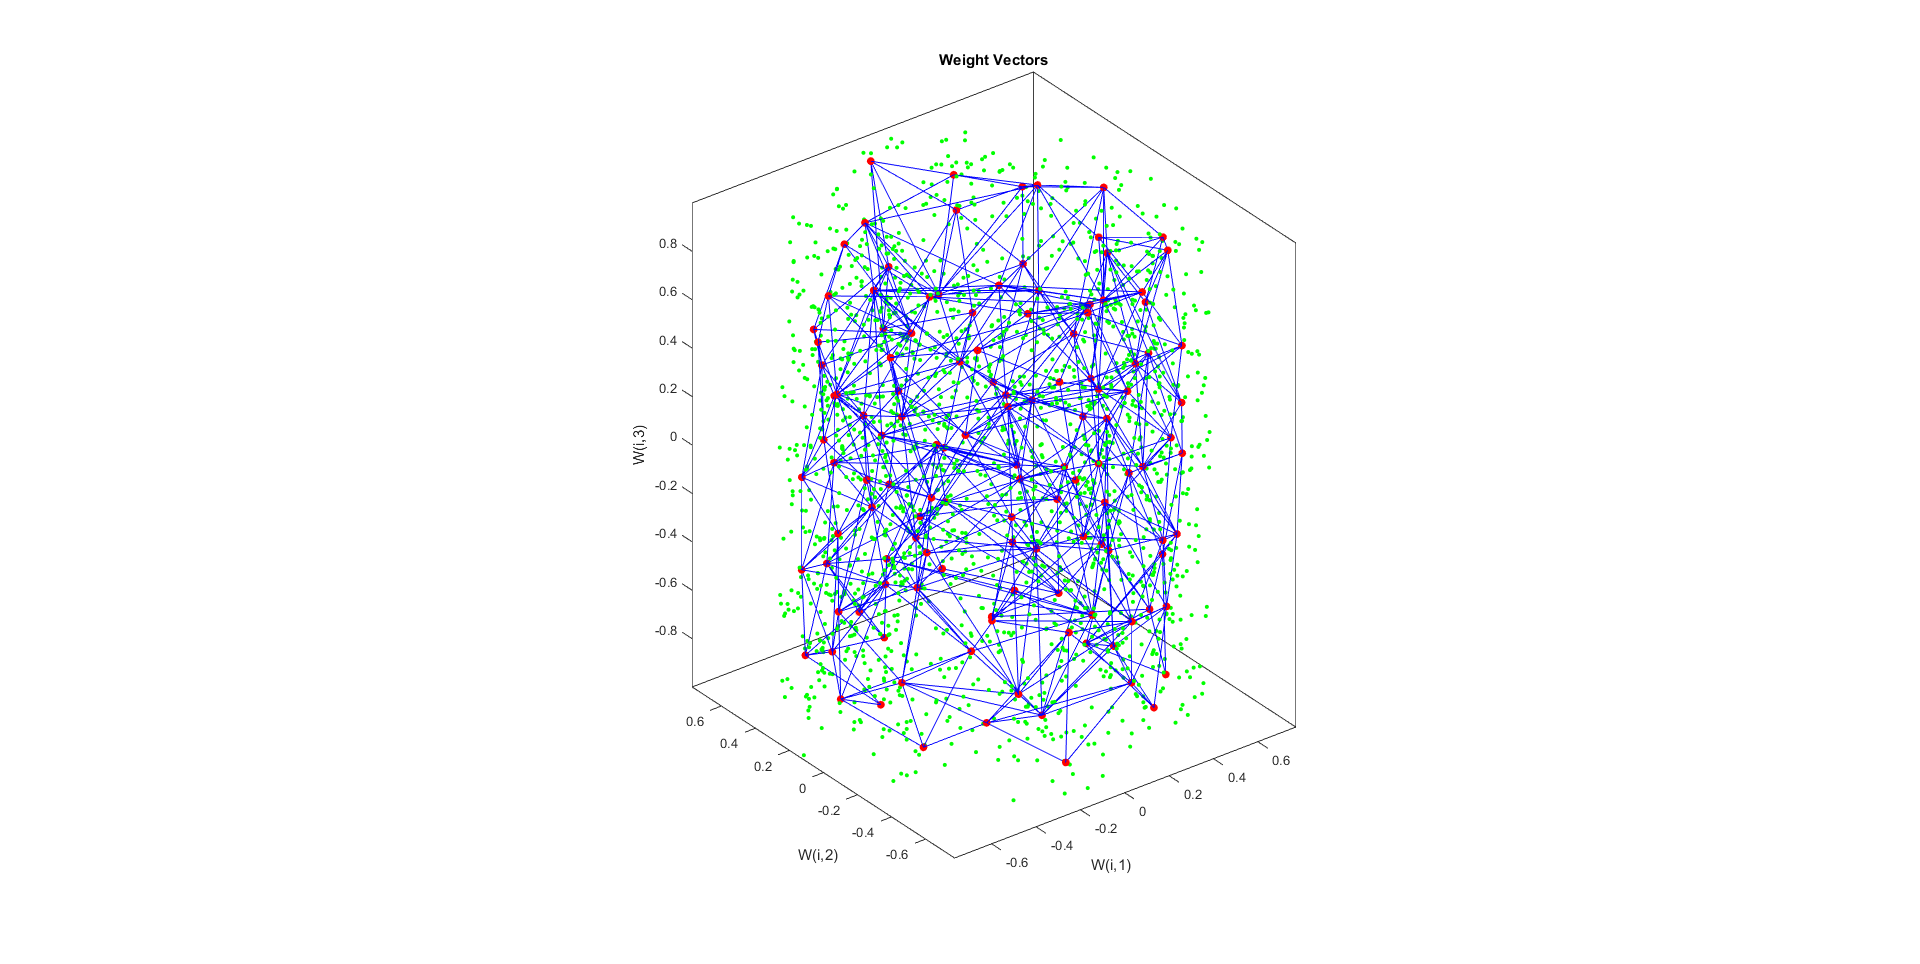
\includegraphics[width=\textwidth/5]{figures_3/som_1000_1} \\
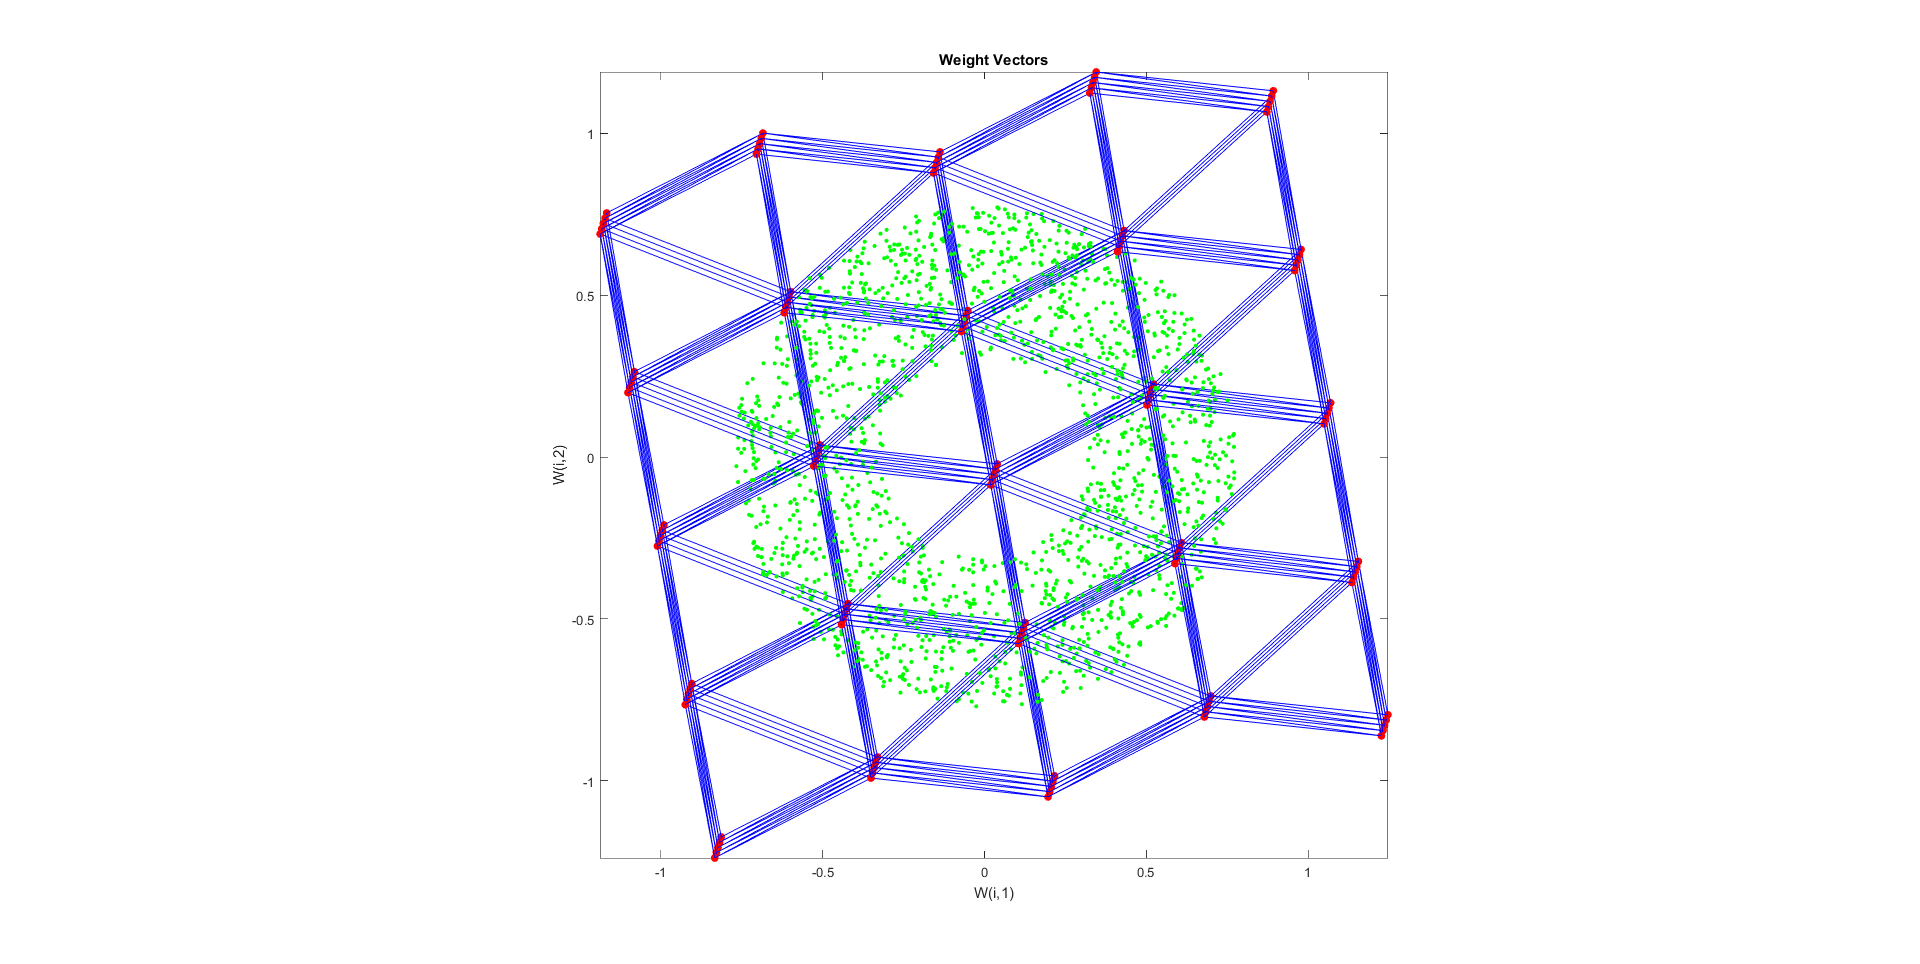
\includegraphics[width=\textwidth/5]{figures_3/som_0_2} &
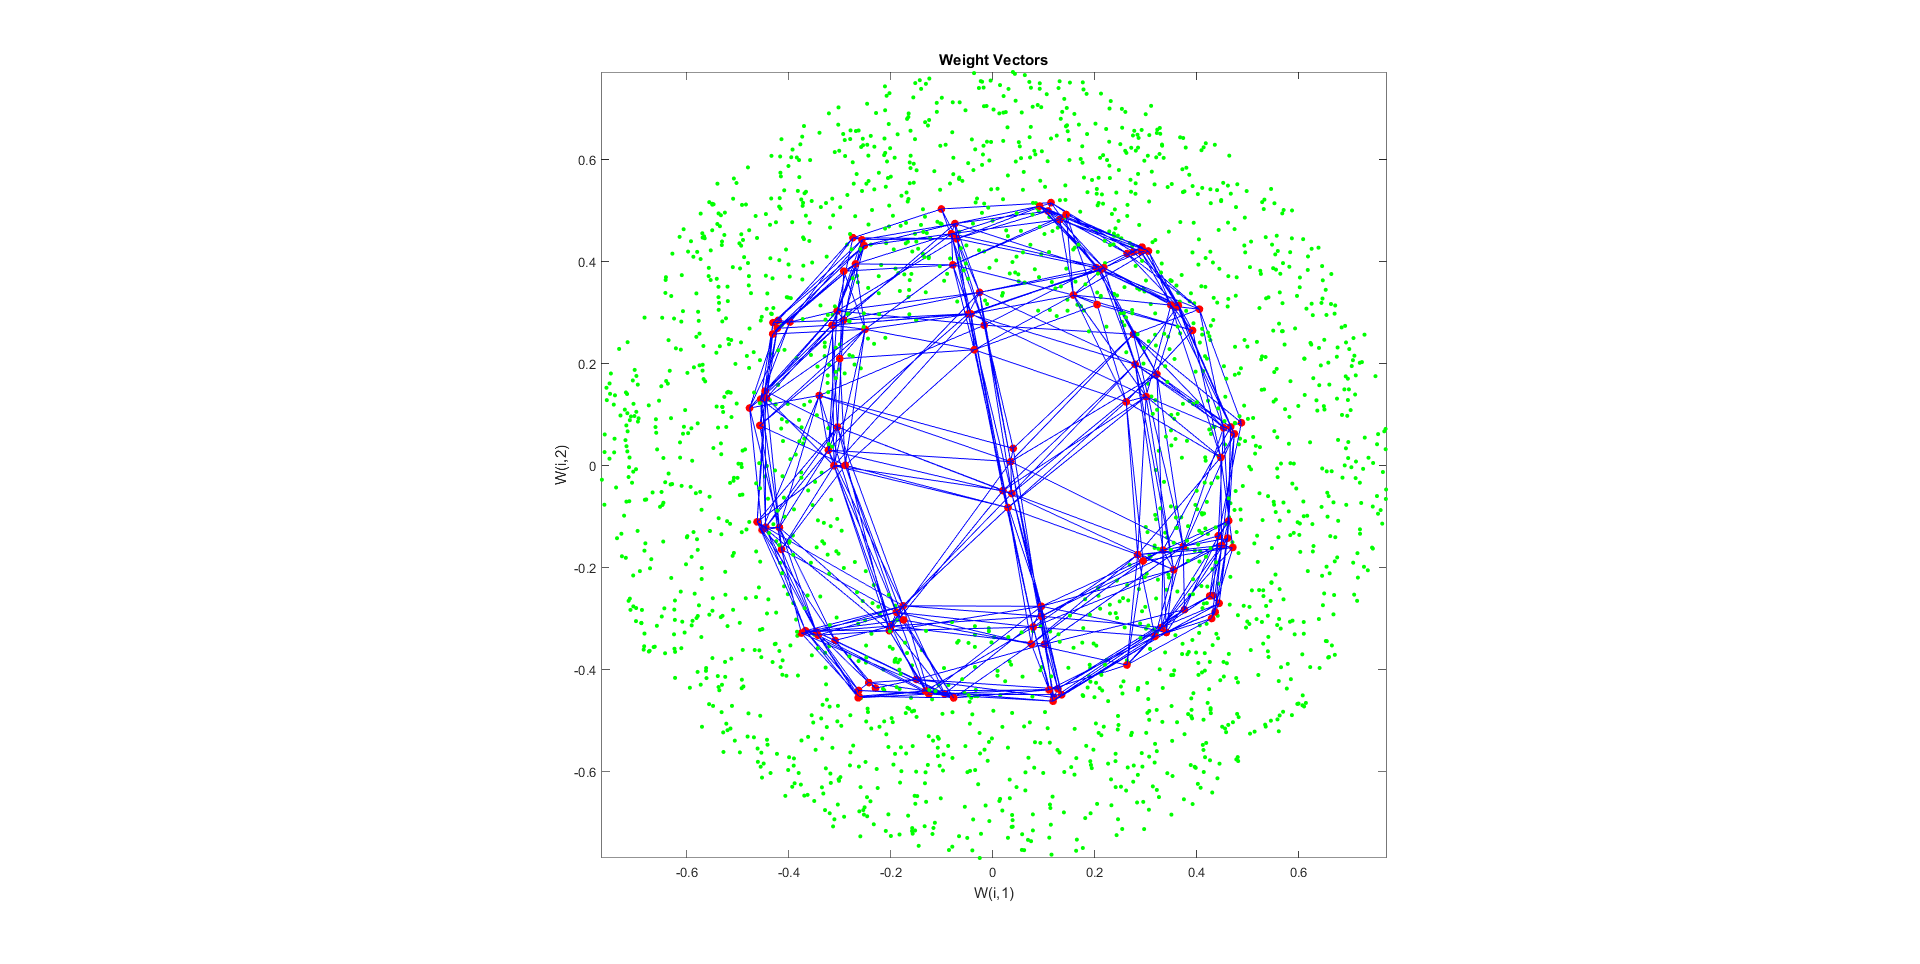
\includegraphics[width=\textwidth/5]{figures_3/som_10_2} &
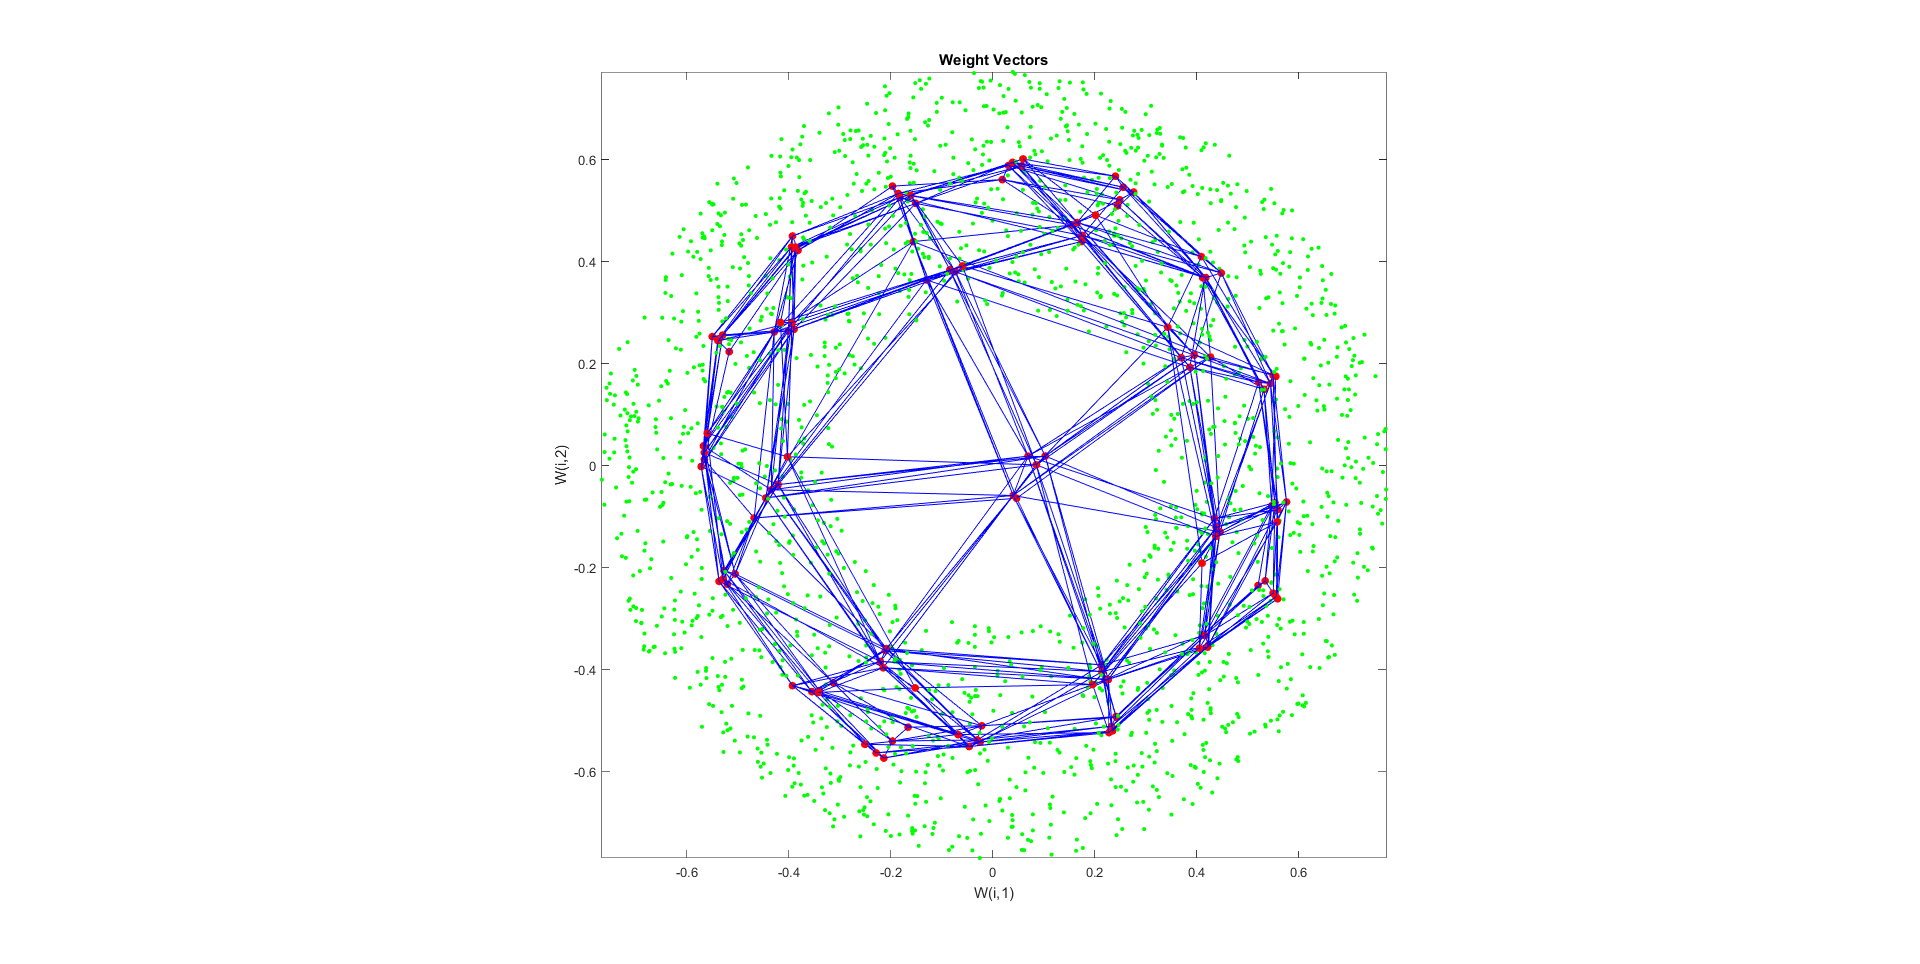
\includegraphics[width=\textwidth/5]{figures_3/som_100_2} &
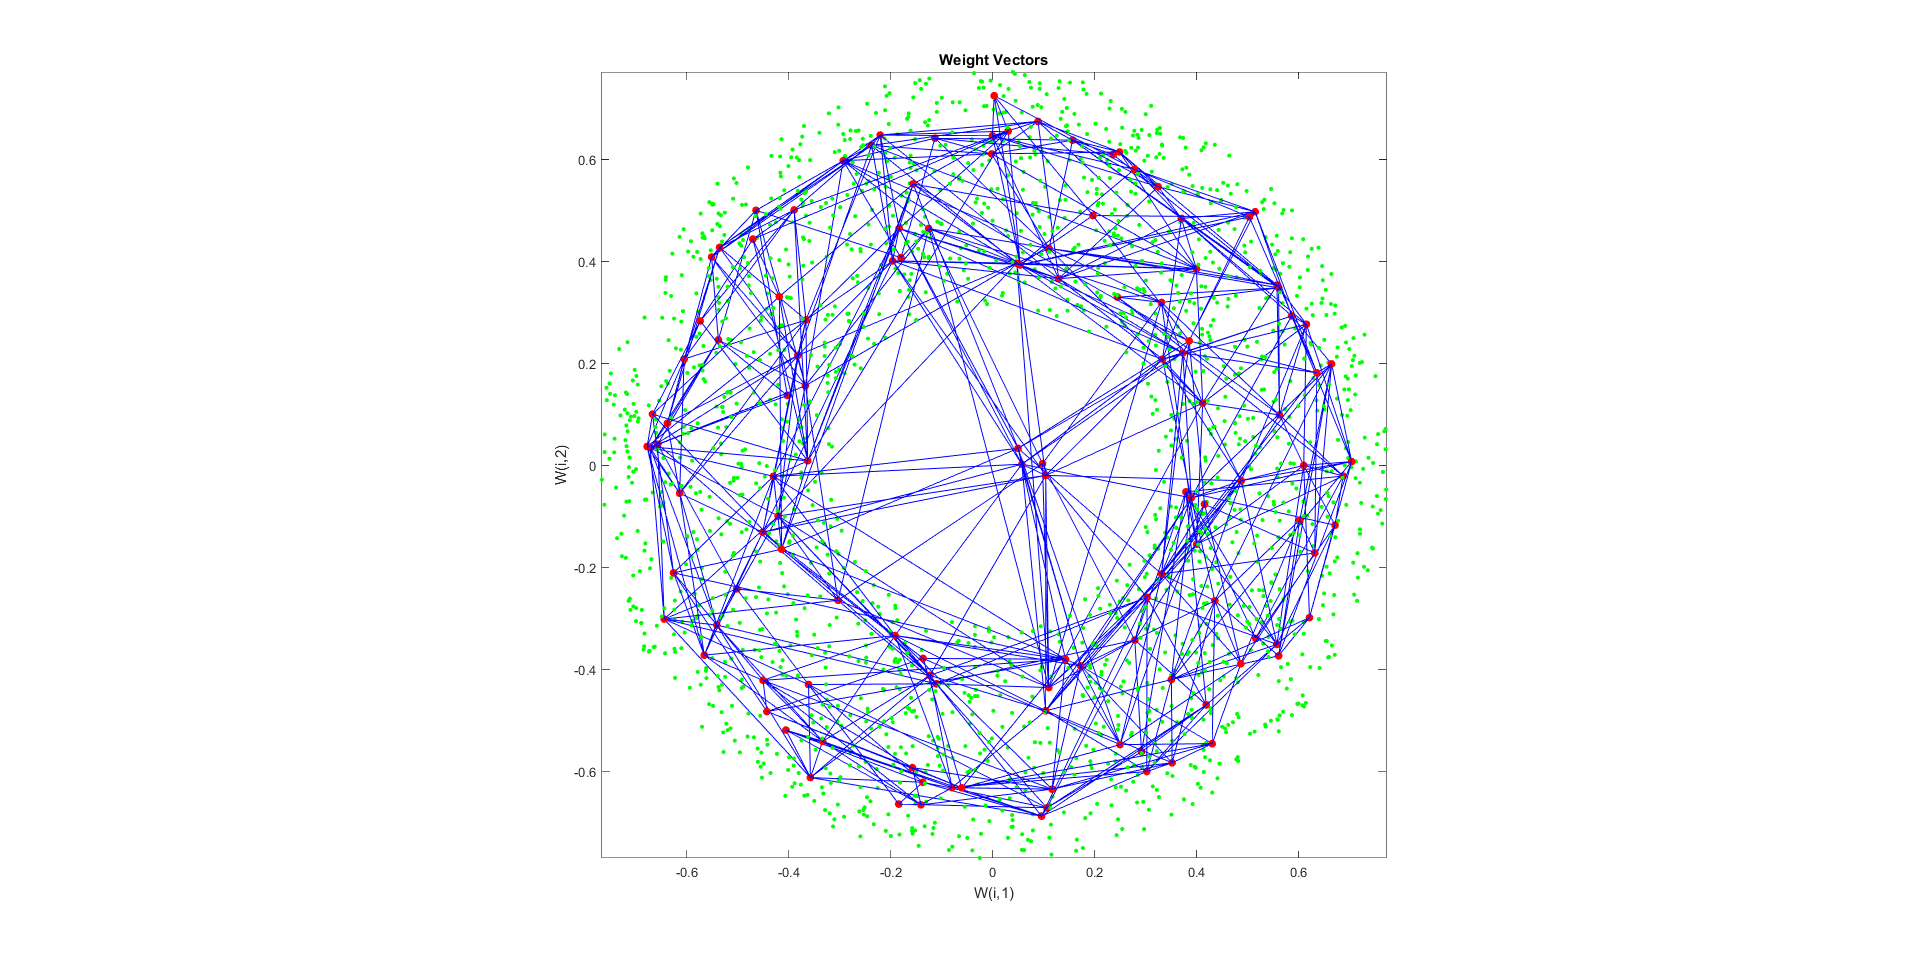
\includegraphics[width=\textwidth/5]{figures_3/som_1000_2} \\

\end{tabular}
\centering
\end{figure}


\begin{figure}[!htbp]
\caption{Top: Plots of SOM using grid topology and \textit{linkdist}. Middle: Plots of SOM using hexagonal topology and \textit{linkdist}. Bottom: Plots of SOM using hexagonal topology and \textit{mandist}.}
\label{panel_22}
\medbreak
\begin{tabular}{ccc}
 
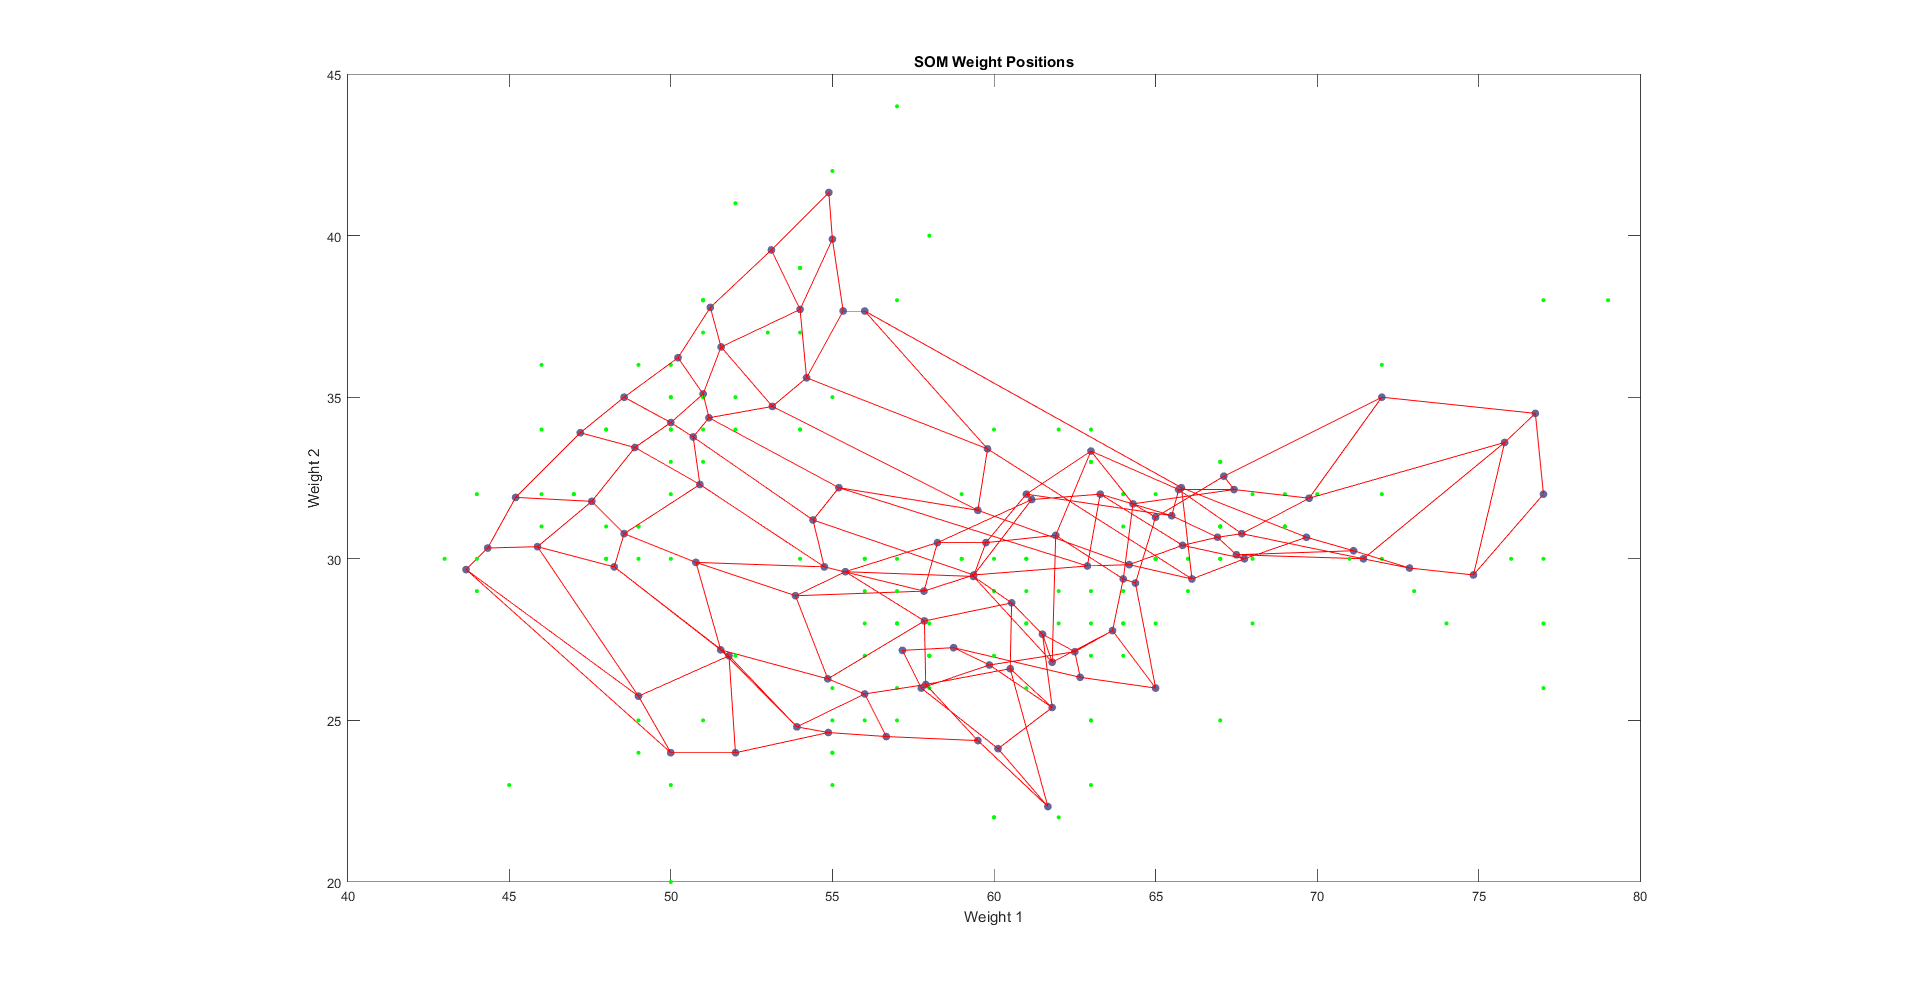
\includegraphics[width=\textwidth/4]{figures_3/som_wp_1} &
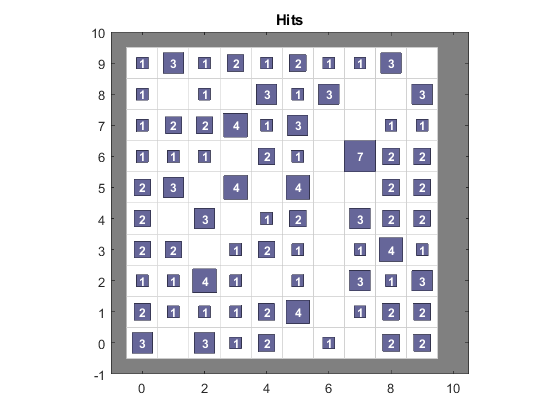
\includegraphics[width=\textwidth/5]{figures_3/som_hits_1} &
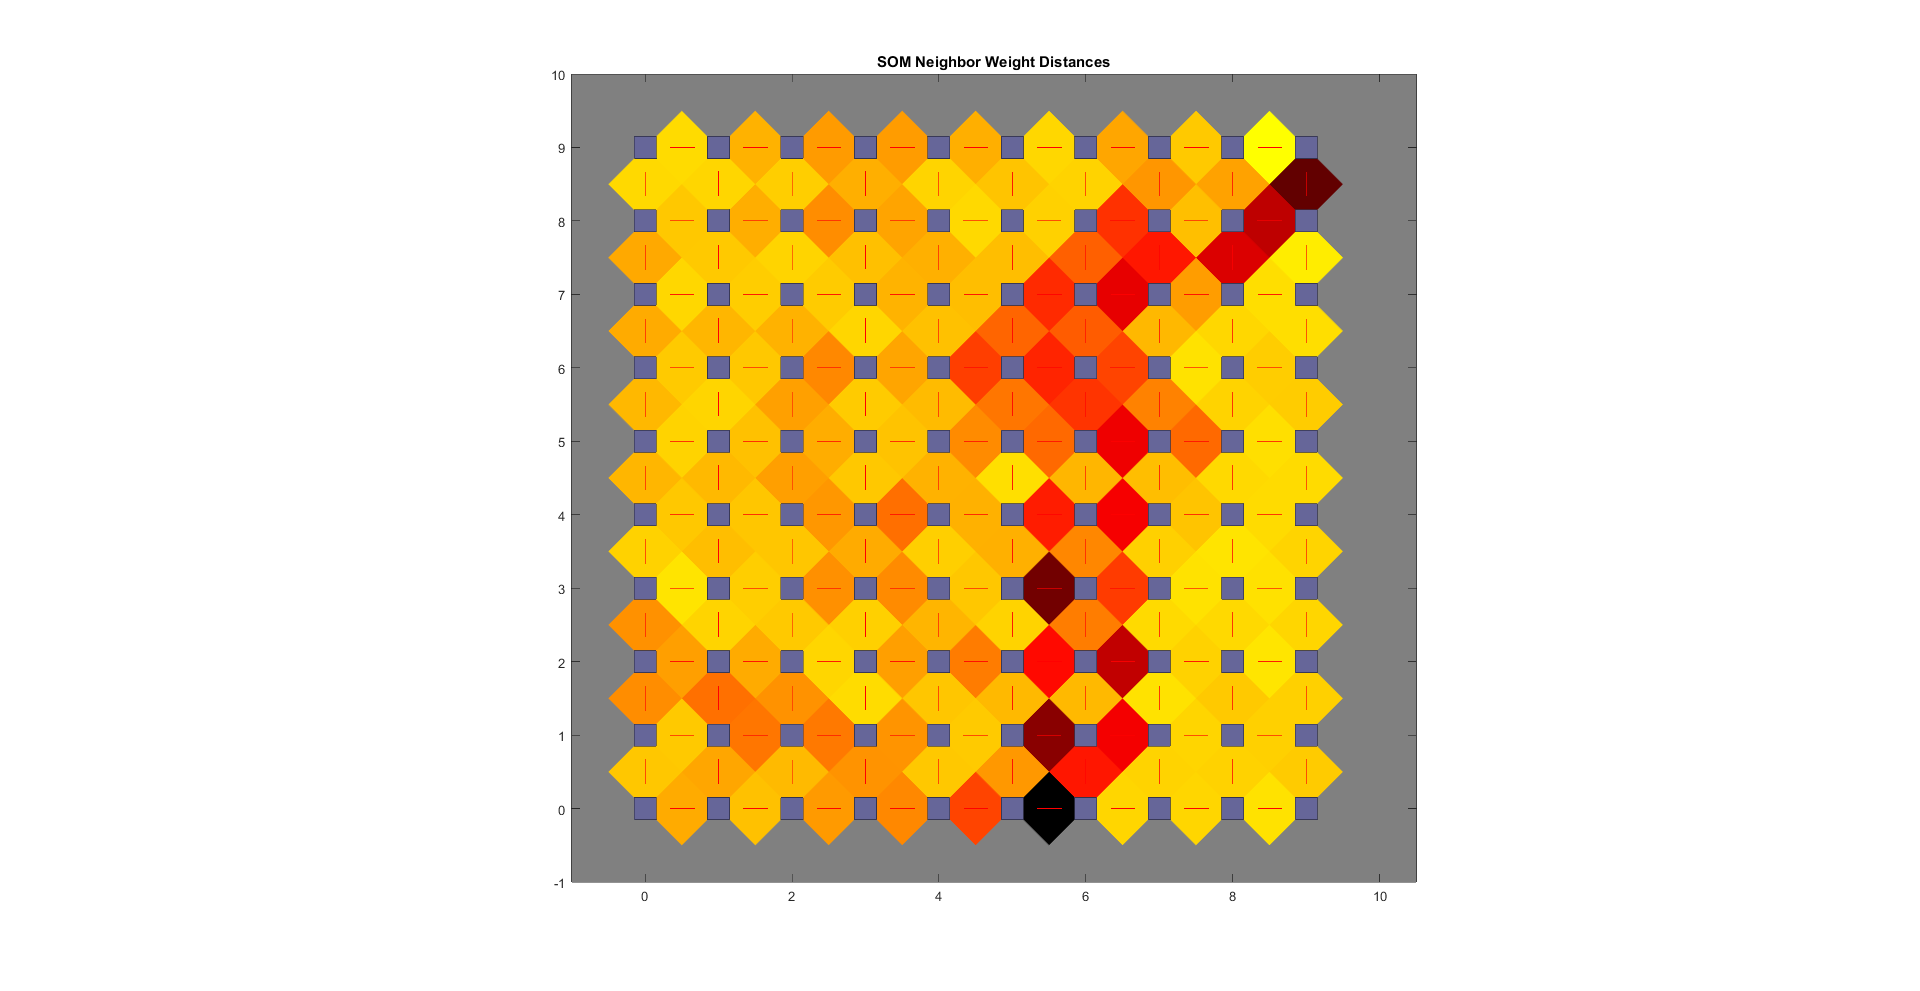
\includegraphics[width=\textwidth/4]{figures_3/som_nwd_1} \\\hline

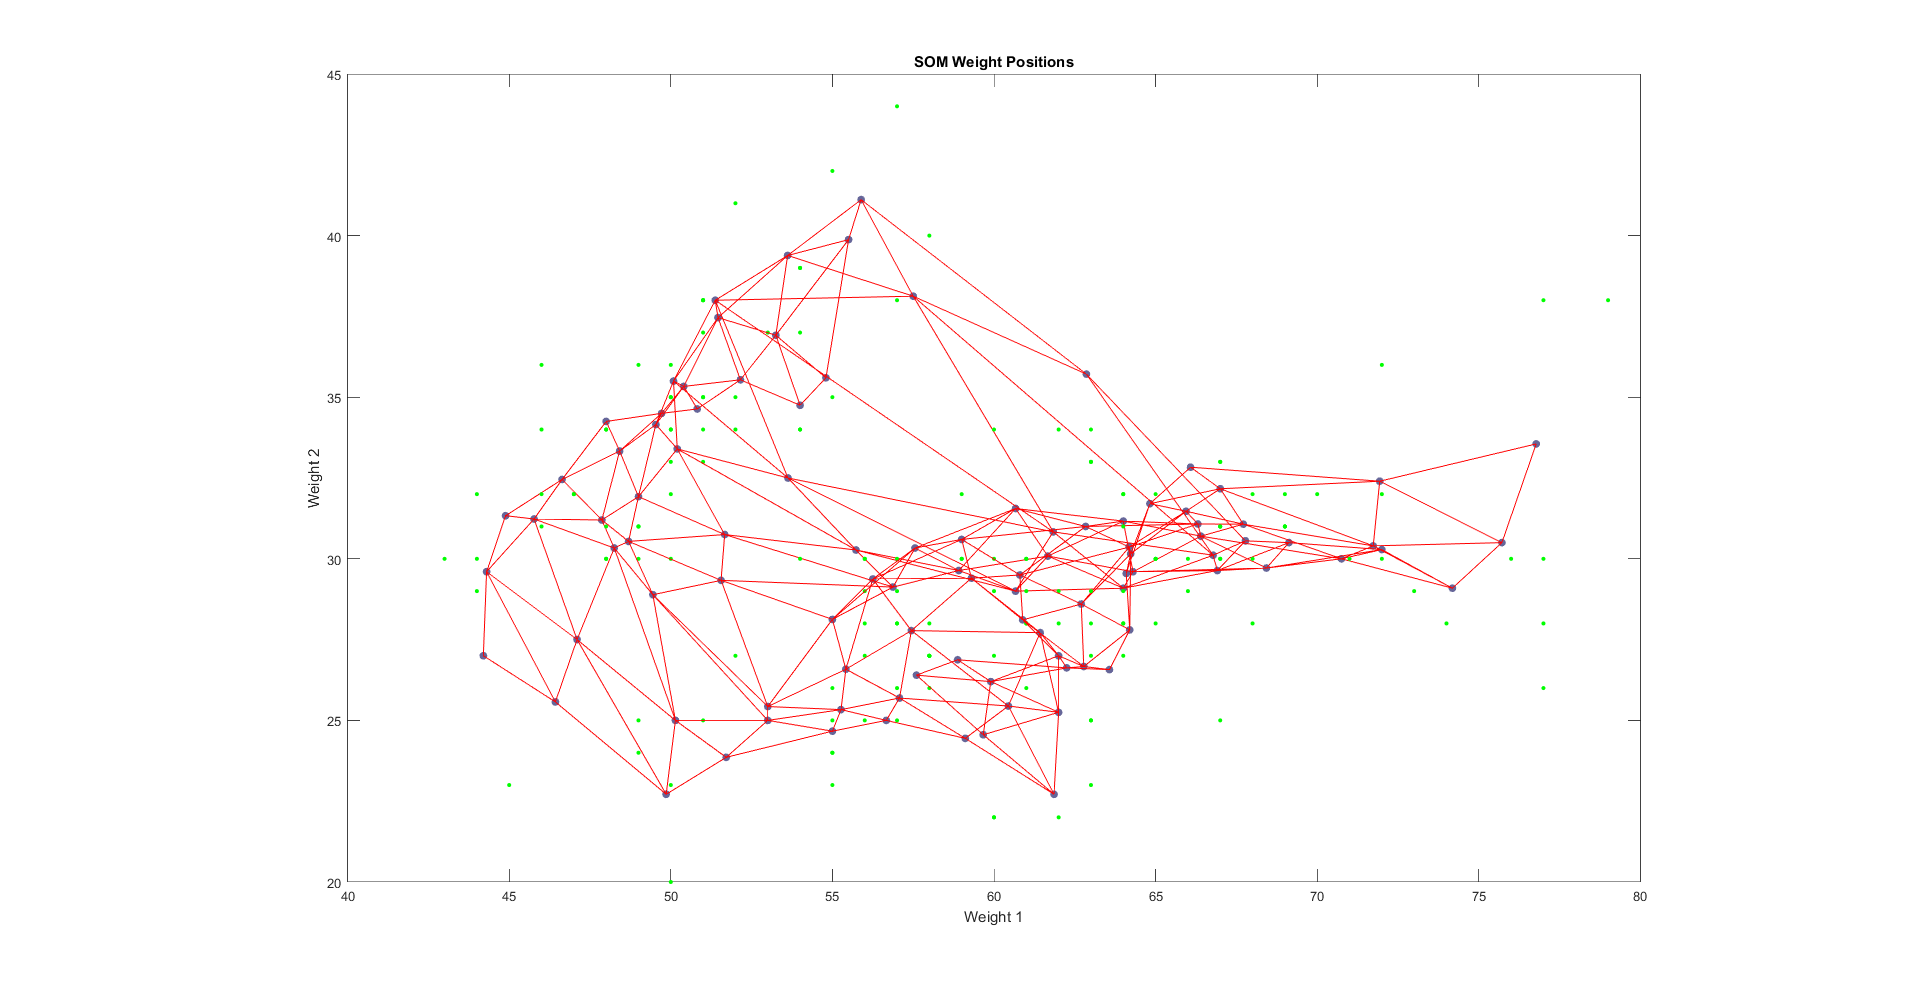
\includegraphics[width=\textwidth/4]{figures_3/som_wp_2} &
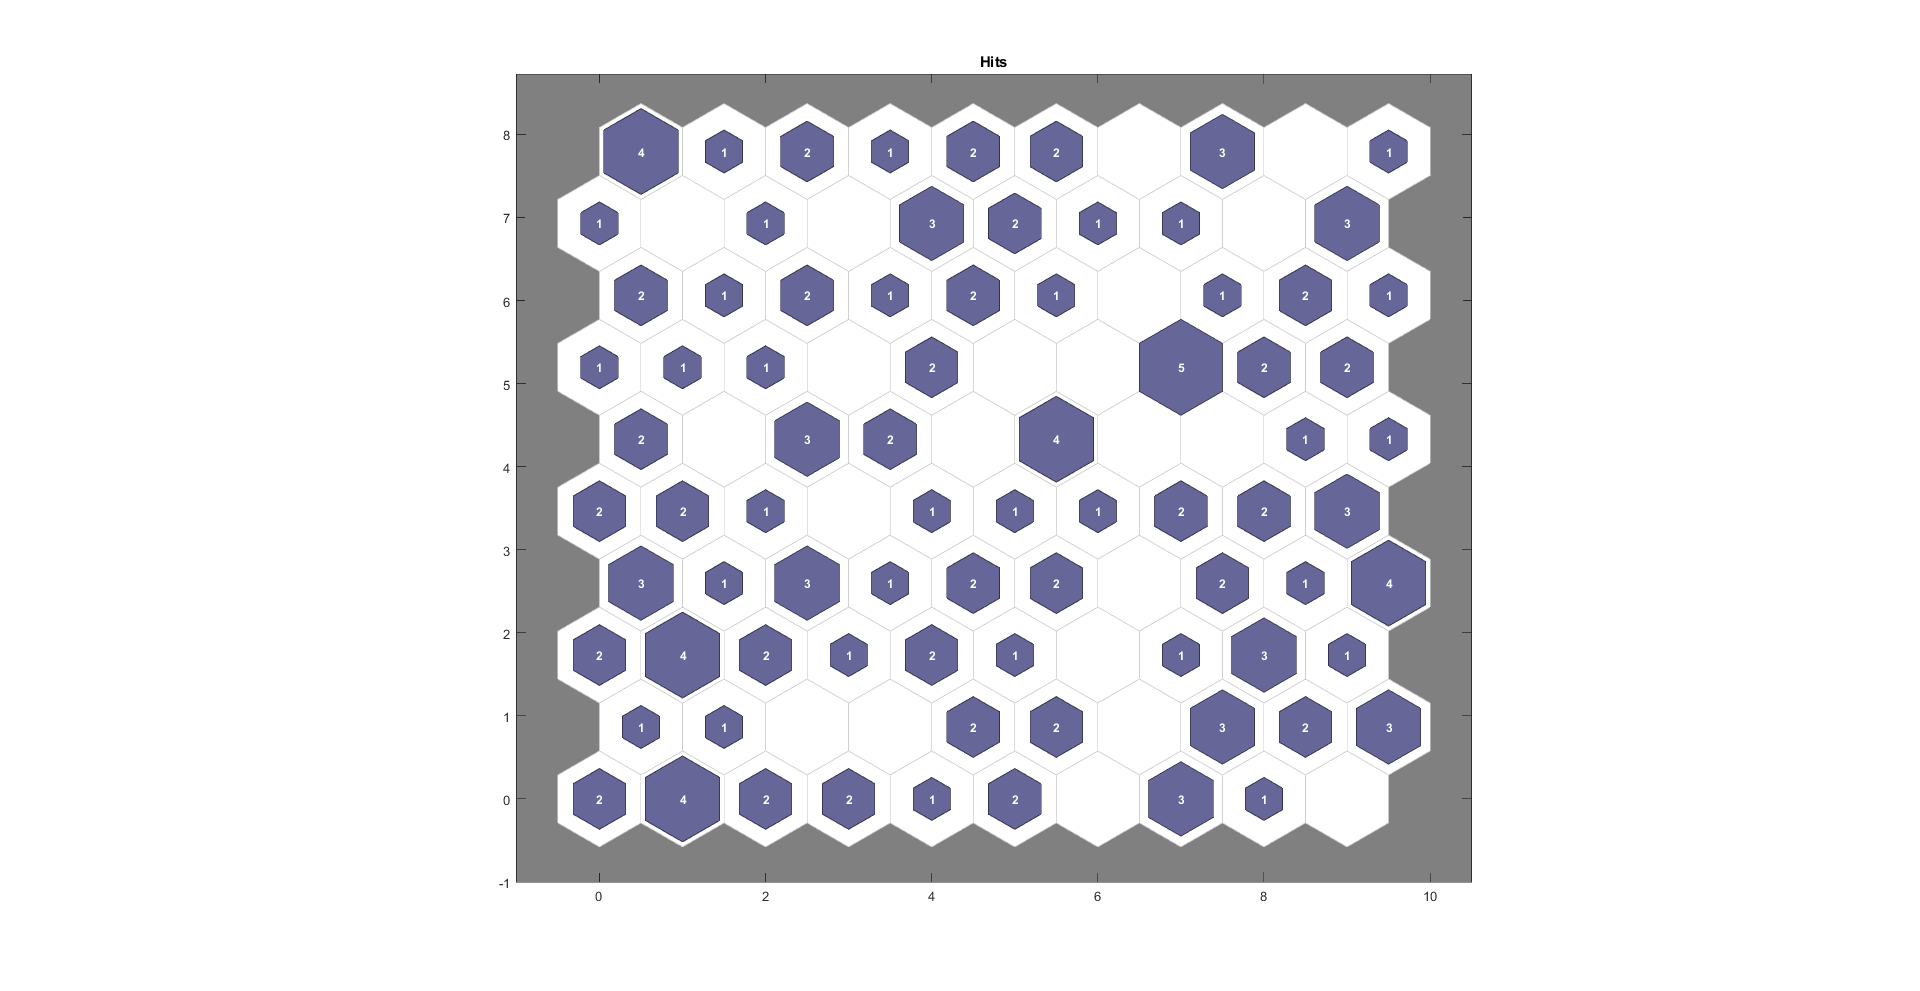
\includegraphics[width=\textwidth/4]{figures_3/som_hits_2} &
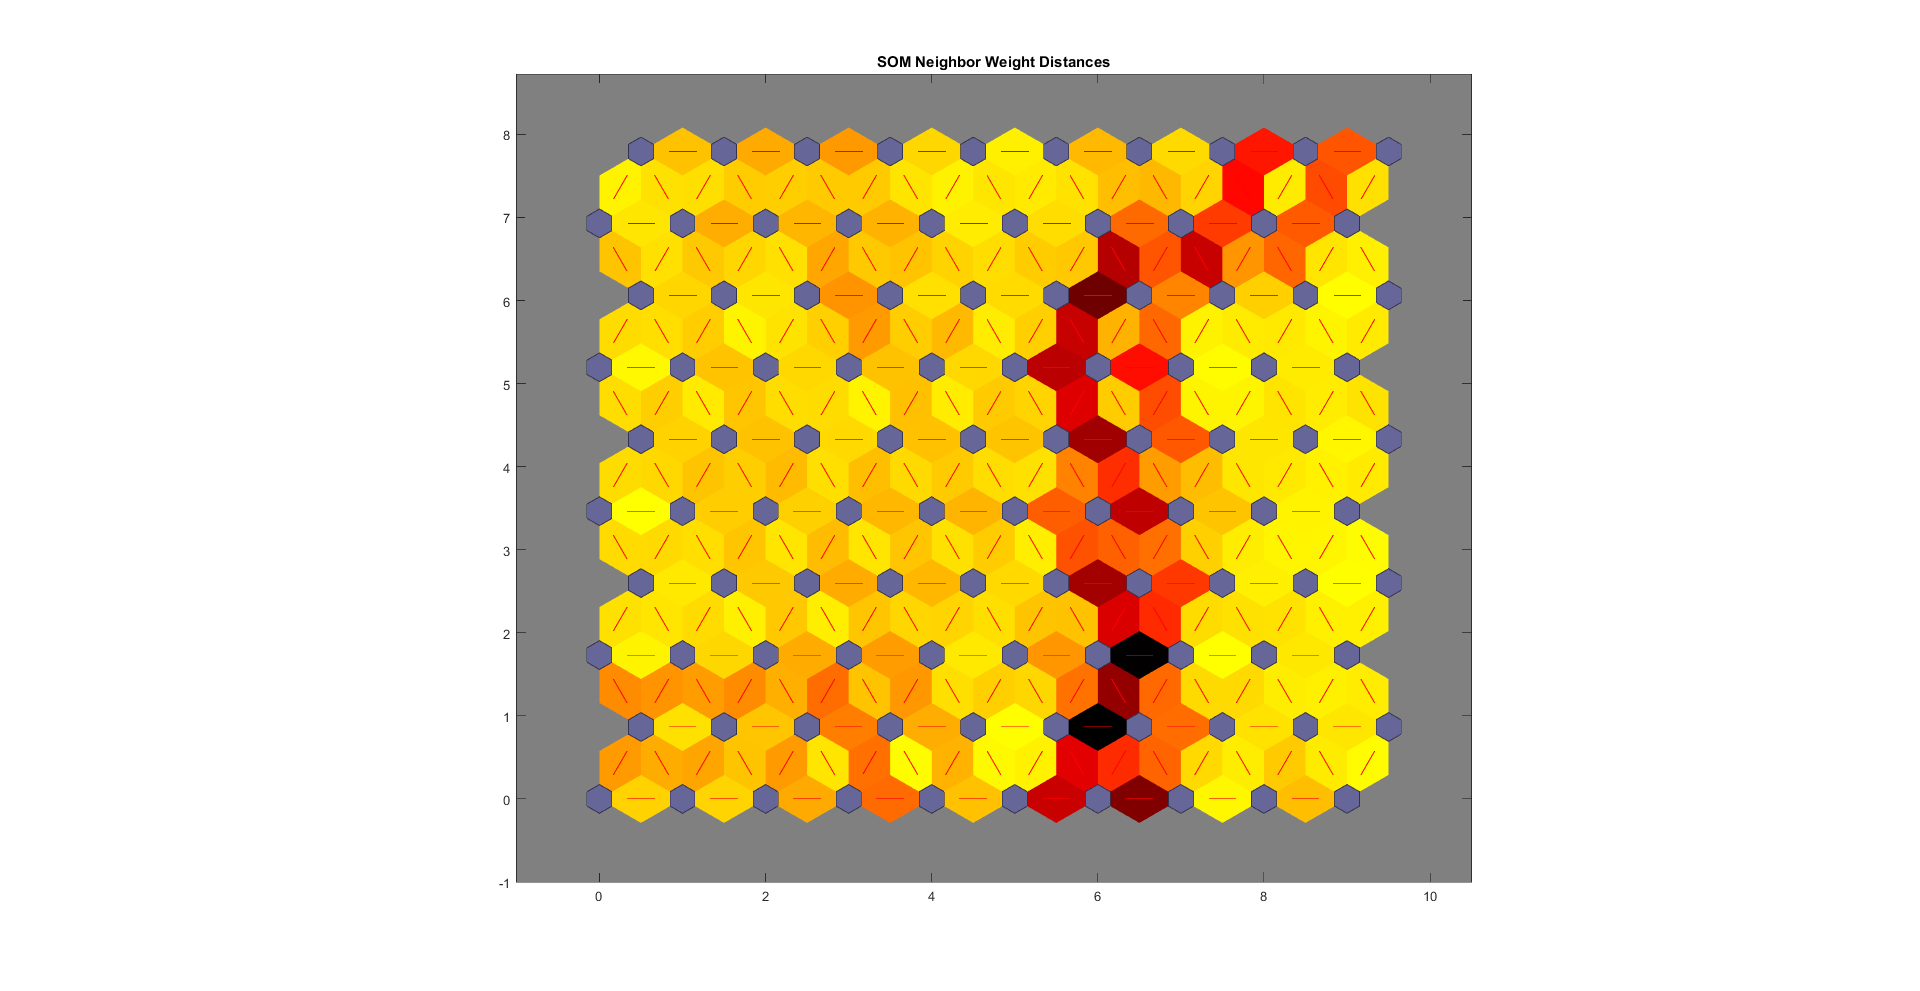
\includegraphics[width=\textwidth/4]{figures_3/som_nwd_2} \\\hline

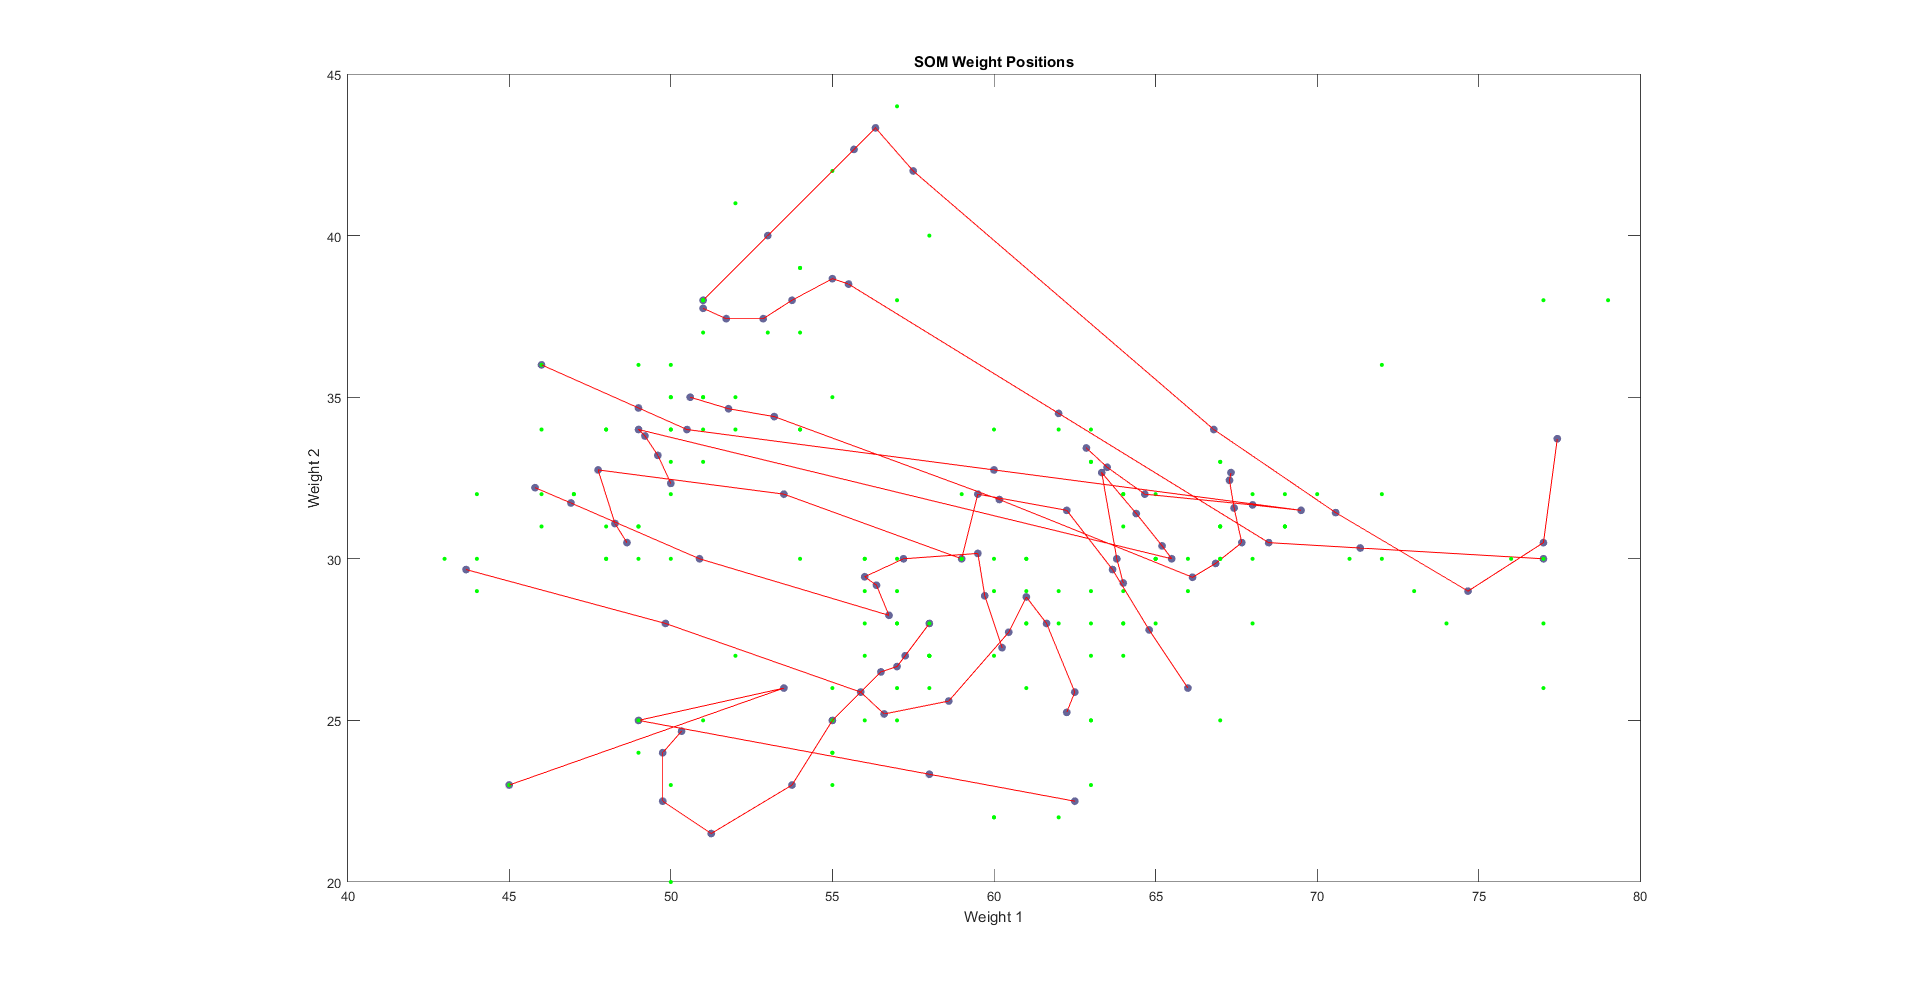
\includegraphics[width=\textwidth/4]{figures_3/som_wp_3} &
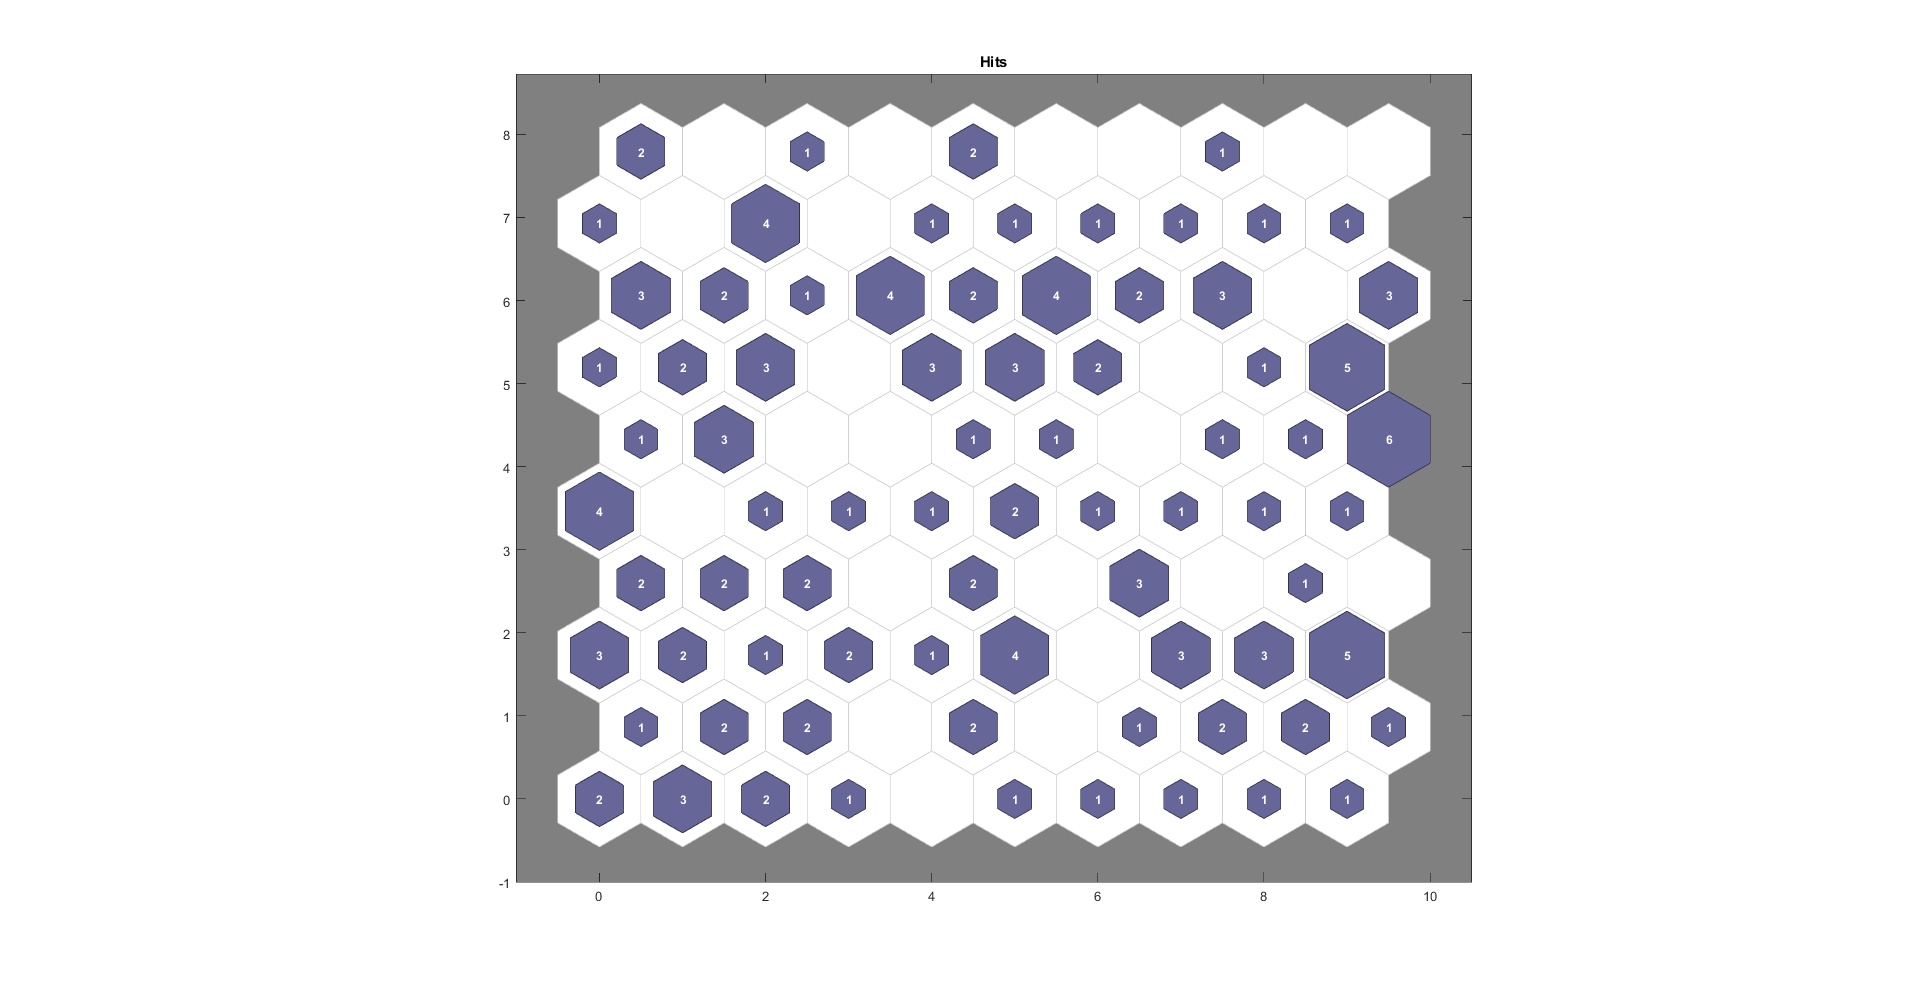
\includegraphics[width=\textwidth/4]{figures_3/som_hits_3} &
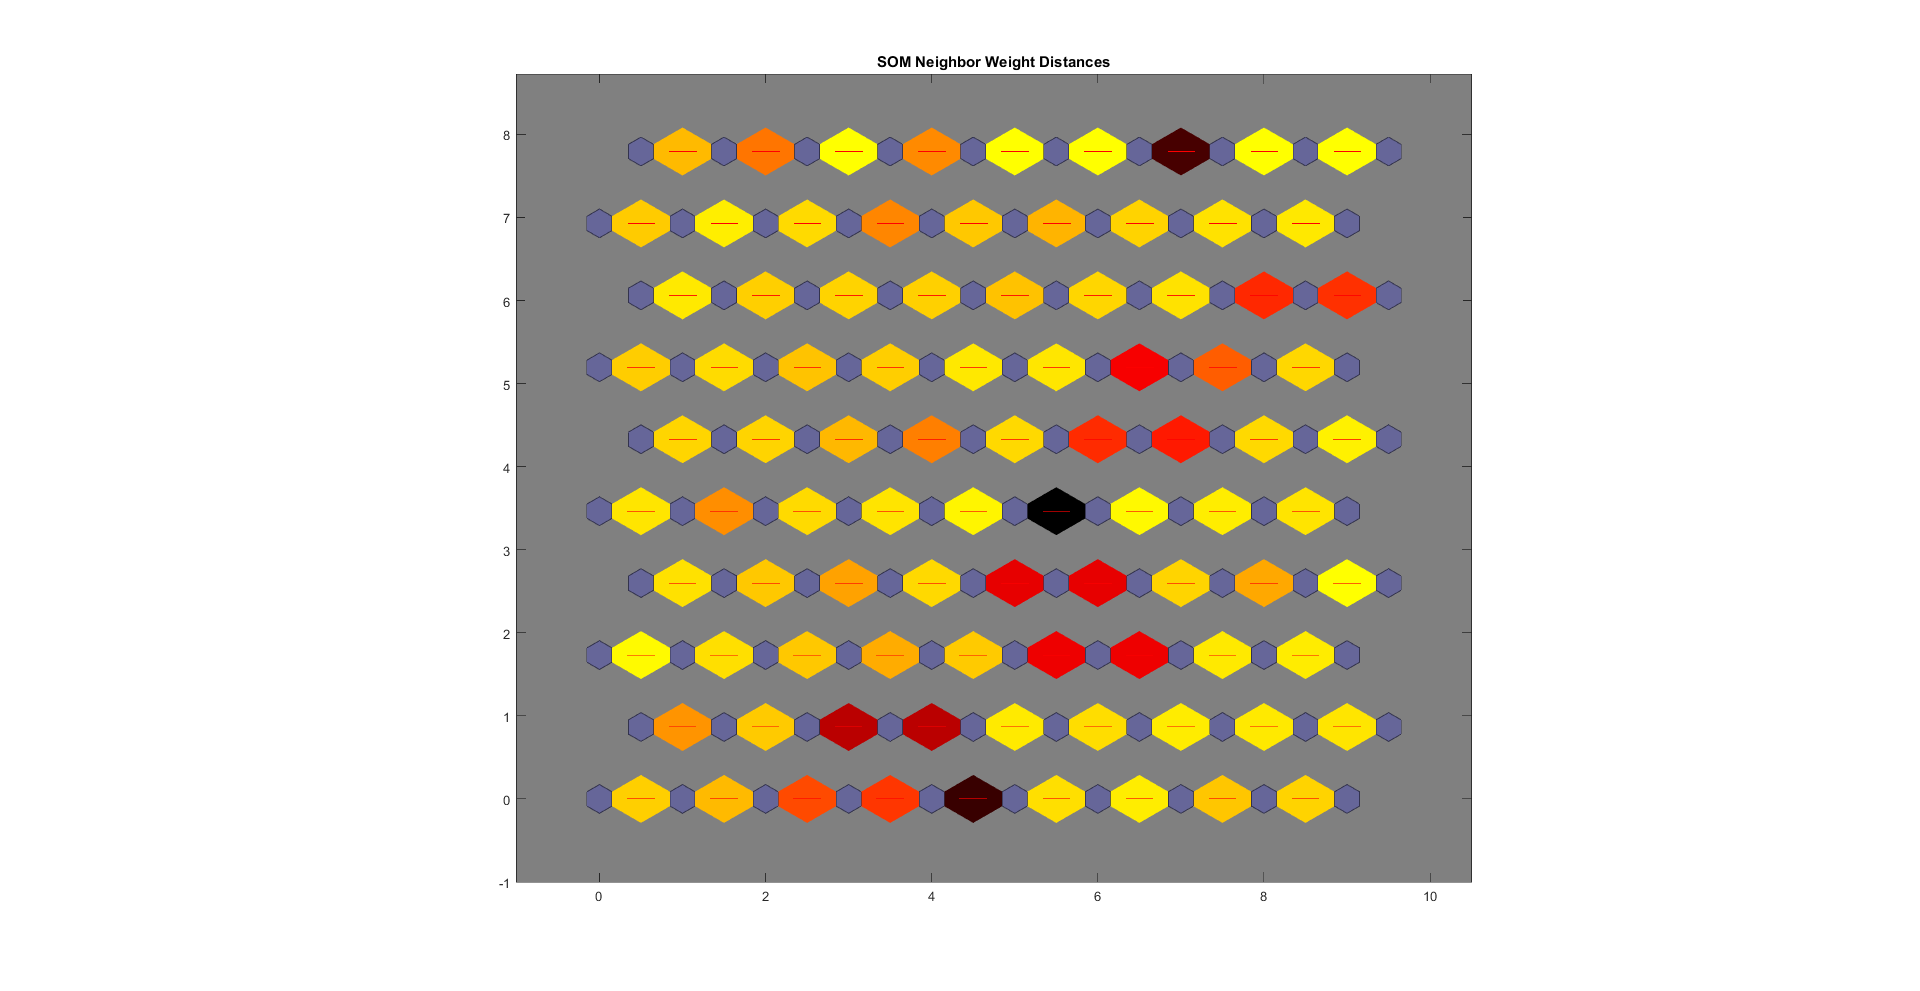
\includegraphics[width=\textwidth/4]{figures_3/som_nwd_3} \\\hline
\end{tabular}
\centering
\end{figure}

\newpage
\section{S4: Deep Learning: stacked autoencoders and convolutional Neural networks}
\subsection{Stacked autoencoders}
After analyzed \textbf{DigitClassification.m} script, several experiments were run. Tables \ref{table_sec_4_1} and \ref{table_sec_4_2} show the results of different models with different hyperparameters.
\bigbreak
All the models could beat the original one (second column in table \ref{table_sec_4_1}) but the model with third hidden layers (seventh column in table \ref{table_sec_4_1}) before the fined-tuning. However after the fined-tuning, the DeppNets could not overcome the original setting. Even the best model (fifth column in table \ref{table_sec_4_1}) was not able to perform better.
\bigbreak
Three interesting remark are noticed. The model with best results after fined-tuning took around 7 minutes per run. That is a significant amount of time compared with the other models, even the second best model before fined-tuning (sixth column in table \ref{table_sec_4_1}) took around 3 minutes per run. This is a extensive impact in the time complexity of the overall model where the gain was relatively small (1.03). Is really it a good tradeoff between time and accuracy?. It precisely depends on the application, for instance in applications where the accuracy is highly important such as the health-care sector.
\bigbreak
However, this tradeoff between time and accuracy can be easily solved using the fined-tuning phase. Clearly the results shown that the fined-tuning phase improve all models, even the worst model that used 3 hidden layers. It was completely not expected that the accuracy of the models improved to beat even the FFNN. Fined-tuning phase has shown that is an important phase in order to improve, even in the worst cases, the accuracy of the model.
\bigbreak
Finally, after fined-tuning all the models beat the FFNN with 1 and 2 layers. However the overall performance are not bad whatsoever. Reaching an average of 96.94 and 96.45, FFNN has shown that it is a very powerful as well as a simple model. As aforementioned, FFNN can be implemented in many applications that do not require heavy critical decision.
\begin{table}[!htbp]
\centering
\caption{Results of DeepNet before fined-tuning. (\# layer, max epochs, hidden units)}
\label{table_sec_4_1}
\medbreak
\begin{tabular}{c|c|c|c|c|c|c}
 & \pbox{4cm}{1, 400, 100\\2, 100, 50} & \pbox{4cm}{1, 400, 100\\2, 400, 50} & \pbox{4cm}{1, 100, 100\\2, 400, 50} & \pbox{4cm}{1, 400, 400\\2, 100, 200} & \pbox{4cm}{1, 400, 200\\2, 100, 100} & \pbox{4cm}{1, 400, 100\\2, 100, 50\\3, 50, 25}\\\hline
1 & 86.72 & 94.16 & 91.28 & 99.18 & 98.24 & 28.84\\\hline
2 & 81.18 & 94.70 & 93.12 & 99.02 & 97.76 & 29.80\\\hline
3 & 89.16 & 95.36 & 93.70 & 98.32 & 97.84 & 13.68\\\hline
4 & 78.66 & 93.88 & 92.26 & 98.82 & 97.92 & 17.18\\\hline
5 & 82.48 & 92.62 & 91.94 & 98.90 & 97.34 & 17.18\\\hline
\textbf{Avg} & \textbf{83.64} & \textbf{94.14} & \textbf{92.46} & \textbf{98.85} & \textbf{97.82} & \textbf{21.34} 
\end{tabular}
\end{table}


\begin{table}[!htbp]
\centering
\caption{Results of DeepNet after fined-tuning. (\# layer, max epochs, hidden units)}
\label{table_sec_4_2}
\medbreak
\begin{tabular}{c|c|c|c|c|c|c}
 & \pbox{4cm}{1, 400, 100\\2, 100, 50} & \pbox{4cm}{1, 400, 100\\2, 400, 50} & \pbox{4cm}{1, 100, 100\\2, 400, 50} & \pbox{4cm}{1, 400, 400\\2, 100, 200} & \pbox{4cm}{1, 400, 200\\2, 100, 100} & \pbox{4cm}{1, 400, 100\\2, 100, 50\\3, 50, 25}\\\hline
1 & 99.68 & 98.96 & 99.52 & 99.48  &98.86 & 99.24\\\hline
2 & 99.76 & 98.92& 99.52 & 99.56 & 98.88 & 99.30\\\hline
3 & 99.80 & 99.06& 99.52 & 99.10 & 98.36 & 99.32\\\hline
4 & 99.78 & 98.72& 99.54 & 99.20 & 98.04 & 99.32 \\\hline
5 & 99.72 & 98.86 & 99.72 & 99.32 & 99.00 & 99.32\\\hline
\textbf{Avg} & \textbf{99.75} & \textbf{98.90} & \textbf{99.56} & \textbf{99.33} & \textbf{98.64} & \textbf{99.30} 
\end{tabular}
\end{table}


\begin{table}[!htbp]
\centering
\caption{Results using a FFNN.}
\label{table_sec_4_3}
\medbreak
\begin{tabular}{c|c|c}
1 hidden layer & 2 hidden layers \\\hline
1 & 97.02 & 95.84 \\\hline
2 & 96.64 & 97.52 \\\hline
3 & 96.28 & 97.26  \\\hline
4 & 96.28 & 97.26 \\\hline
5 & 97.80 & 94.42 \\\hline
\textbf{Avg} & \textbf{96.94} & \textbf{96.45}
\end{tabular}
\end{table}


\subsection{Convolutional neural networks}
\textbf{What do these weights represent?}
\smallbreak
Hence those weights represent the stack of filtered images. 
\bigbreak
\textbf{What is the dimension of the input at the start of layer 6 and why?}
\smallbreak
The previous layer 5 is a MaxPooing layer. It was found that the \textit{PoolSize} was set to 3x3 pixels and \textit{Stride} to 2x2. For each filtered image in the stack, it reduces the input size from 11x11x3 to 5x5x3. According with the MatLab Documentation \cite{matlab_1}, the attribute \textit{NumChannels} represents the feature maps. In this documentation they states that this input value corresponds to the number of filters in the previous convolutional layer. In this case the number of filter of layer 2 are 96. Hence, the input must take into account the shrunk filtered image by the numbers of filters. The input for layer 6 is of 4 dimensions [5,5,3,96], the same dimensionality than the output of layer 2. An interesting observation is that actually the \textit{NumChannels}  parameter of layer 6 is a vector of [48,48] and not an integer value of 96. According with \cite{matlab_1} this cannot be set manually as a vector, it must be a integer value. I assumed the filters are split due to the CrossChannelNormalizationLayer and Matlab internally accepts that type of input for Layer 6.
\bigbreak
\textbf{What is the final dimension of the problem? How does this compare with the initial dimension?}
\smallbreak
According with the ClassificationOutputLayer, it contains a single vector (1 dimension) that contains 1000 of neurons. The initial dimension was [227,227,3] which gives us a total of 154,587 elements. The reduction clearly is significant, the initial input was reduced roughly 155 times.





\newpage
\section{Final project}
\subsection{P1.1: Nonlinear regression}
Appendix A shows the code used for this assignment. The different set to be used as training, validation and test set were obtained using the built-in command \textit{randperm}. The command was used to generate a random set of numbers from 1 to the size of the dataset. Those become the indices of the numbers to create the final data set. Figure \ref{final_2_1} shows the surface of the training set.
\begin{figure}[!htbp]
\caption{Surface of training set with 1000 elements}
\label{final_2_1}
\medbreak
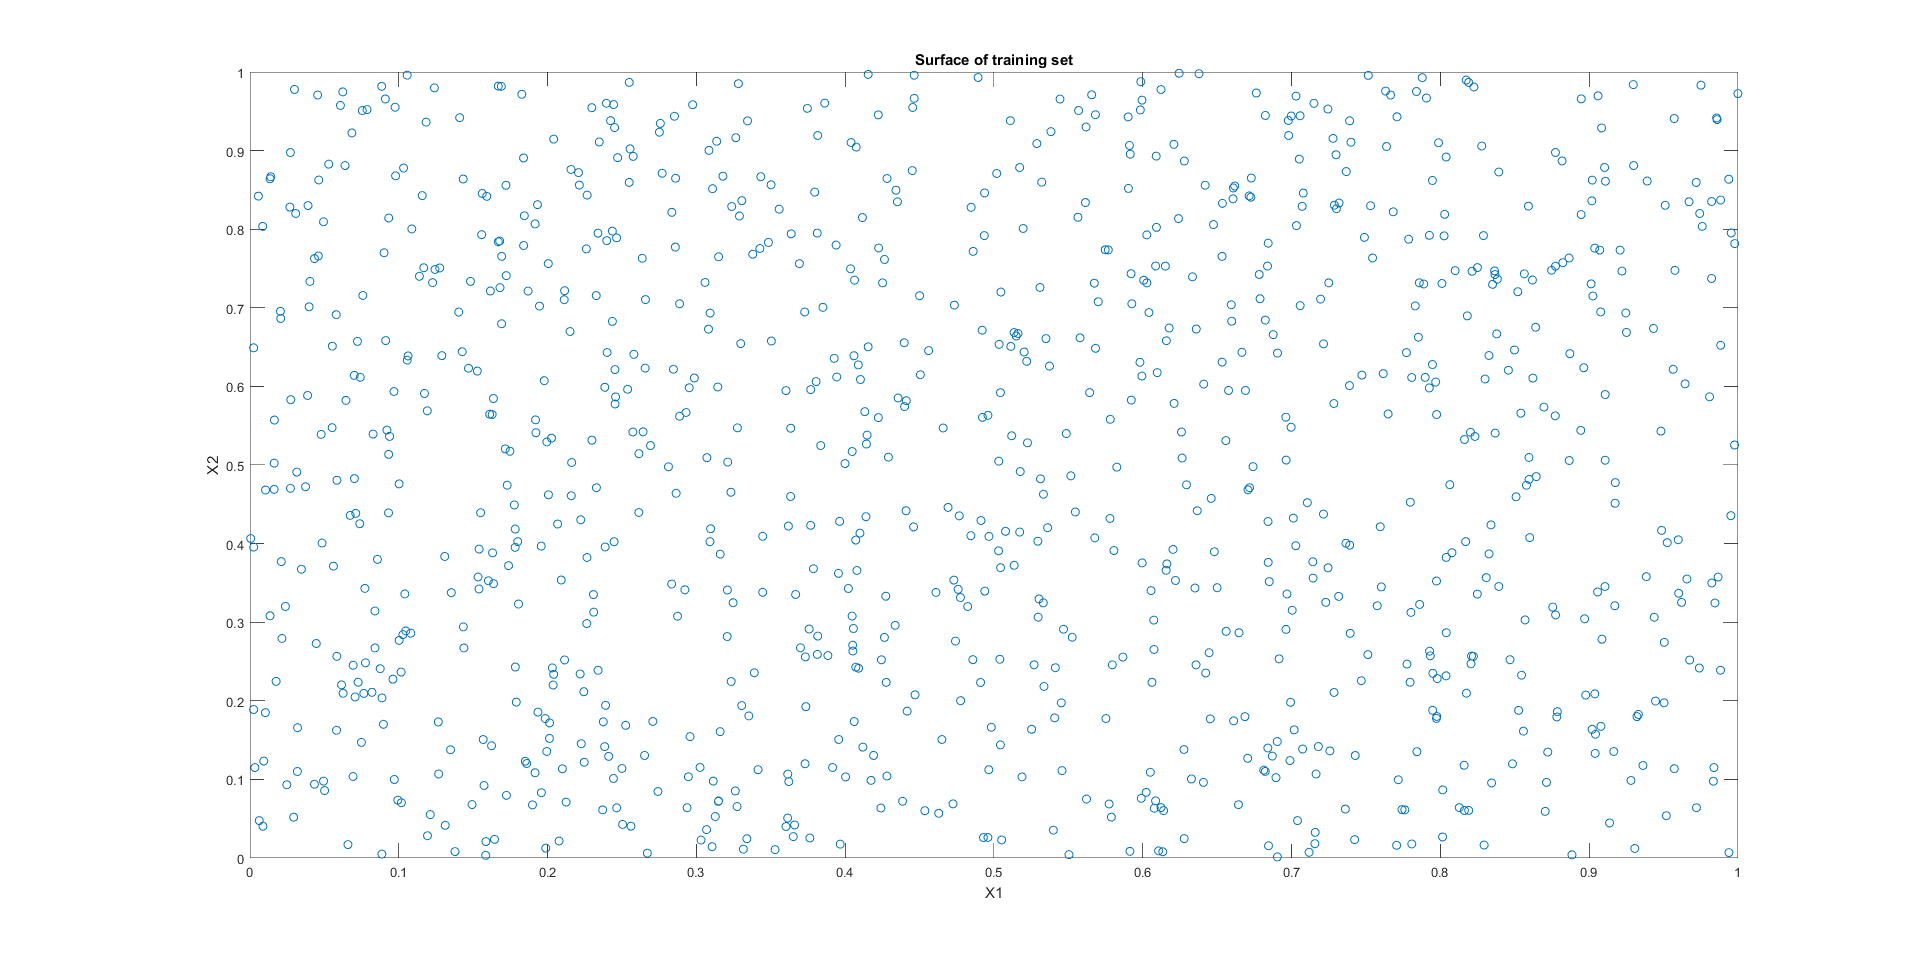
\includegraphics[width=0.9\textwidth]{final/training_set_surface}
\centering
\end{figure}

\begin{figure}[!htbp]
\caption{Plots of FFNN performances with different number of neurons.}
\label{final_2_2}
\medbreak
\begin{tabular}{ccc}
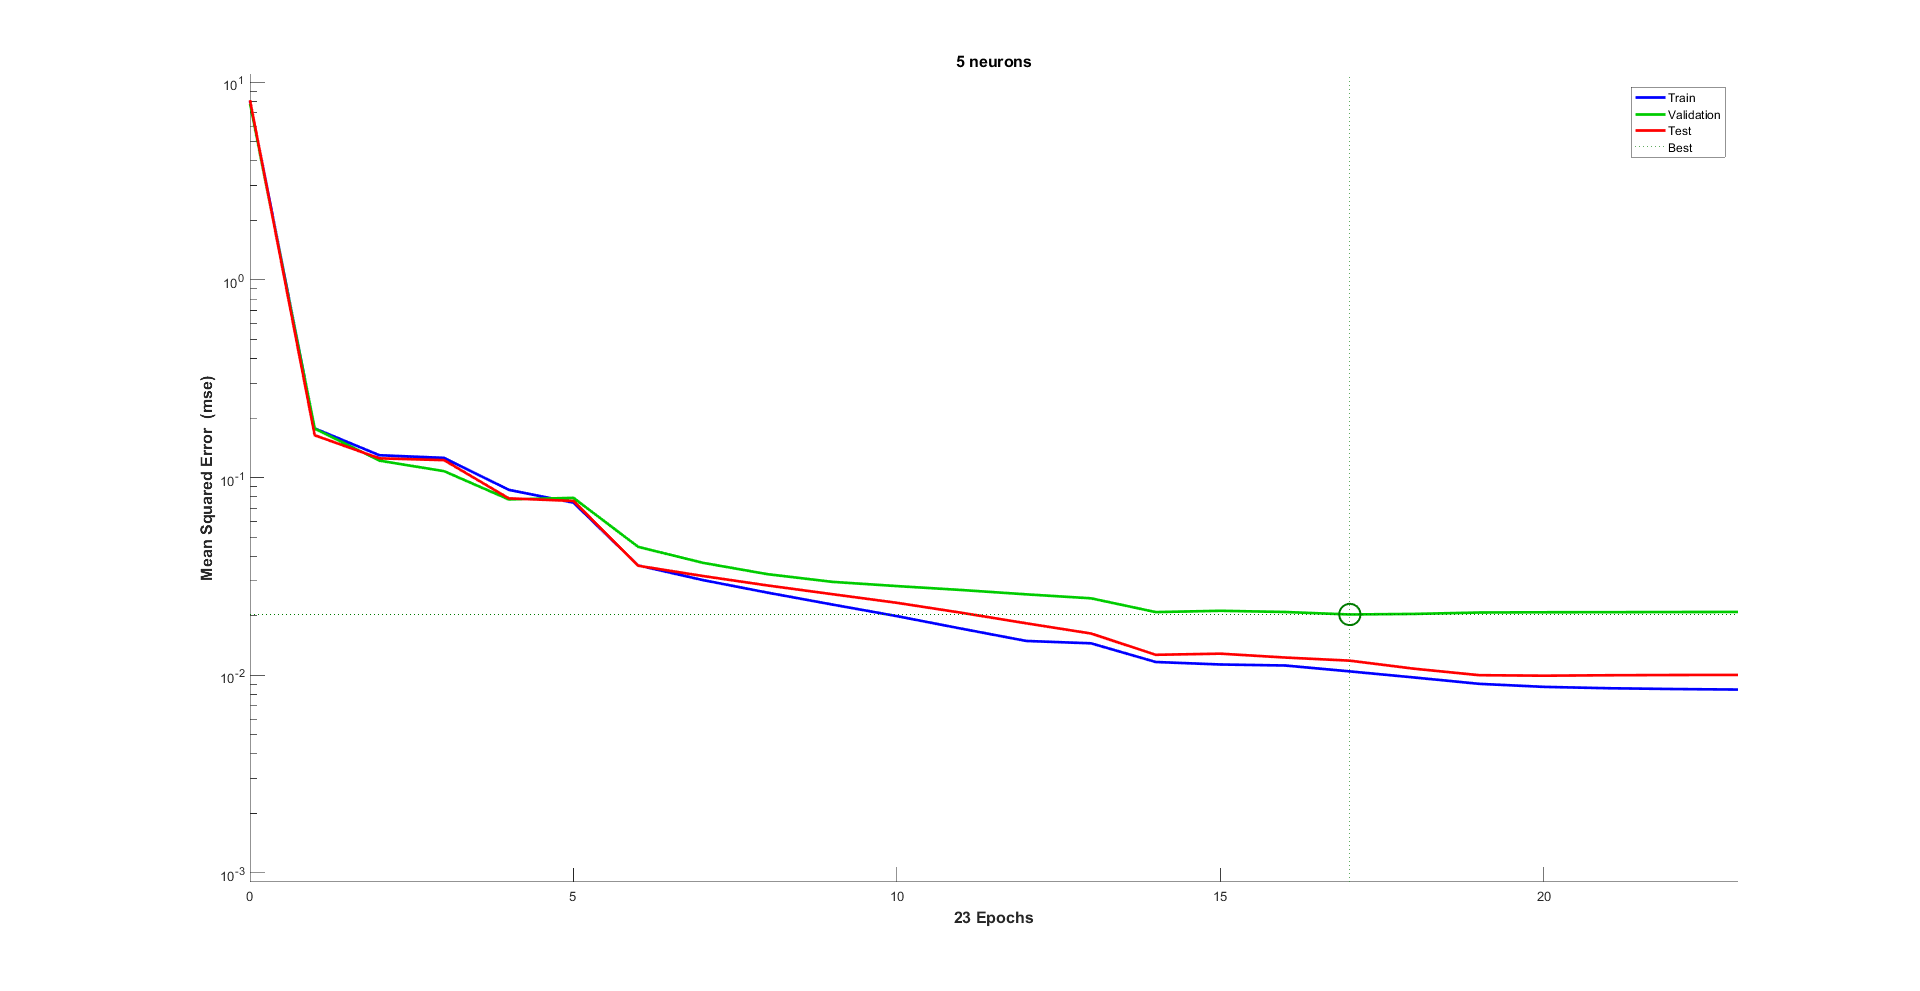
\includegraphics[width=0.45\textwidth]{final/5n} &
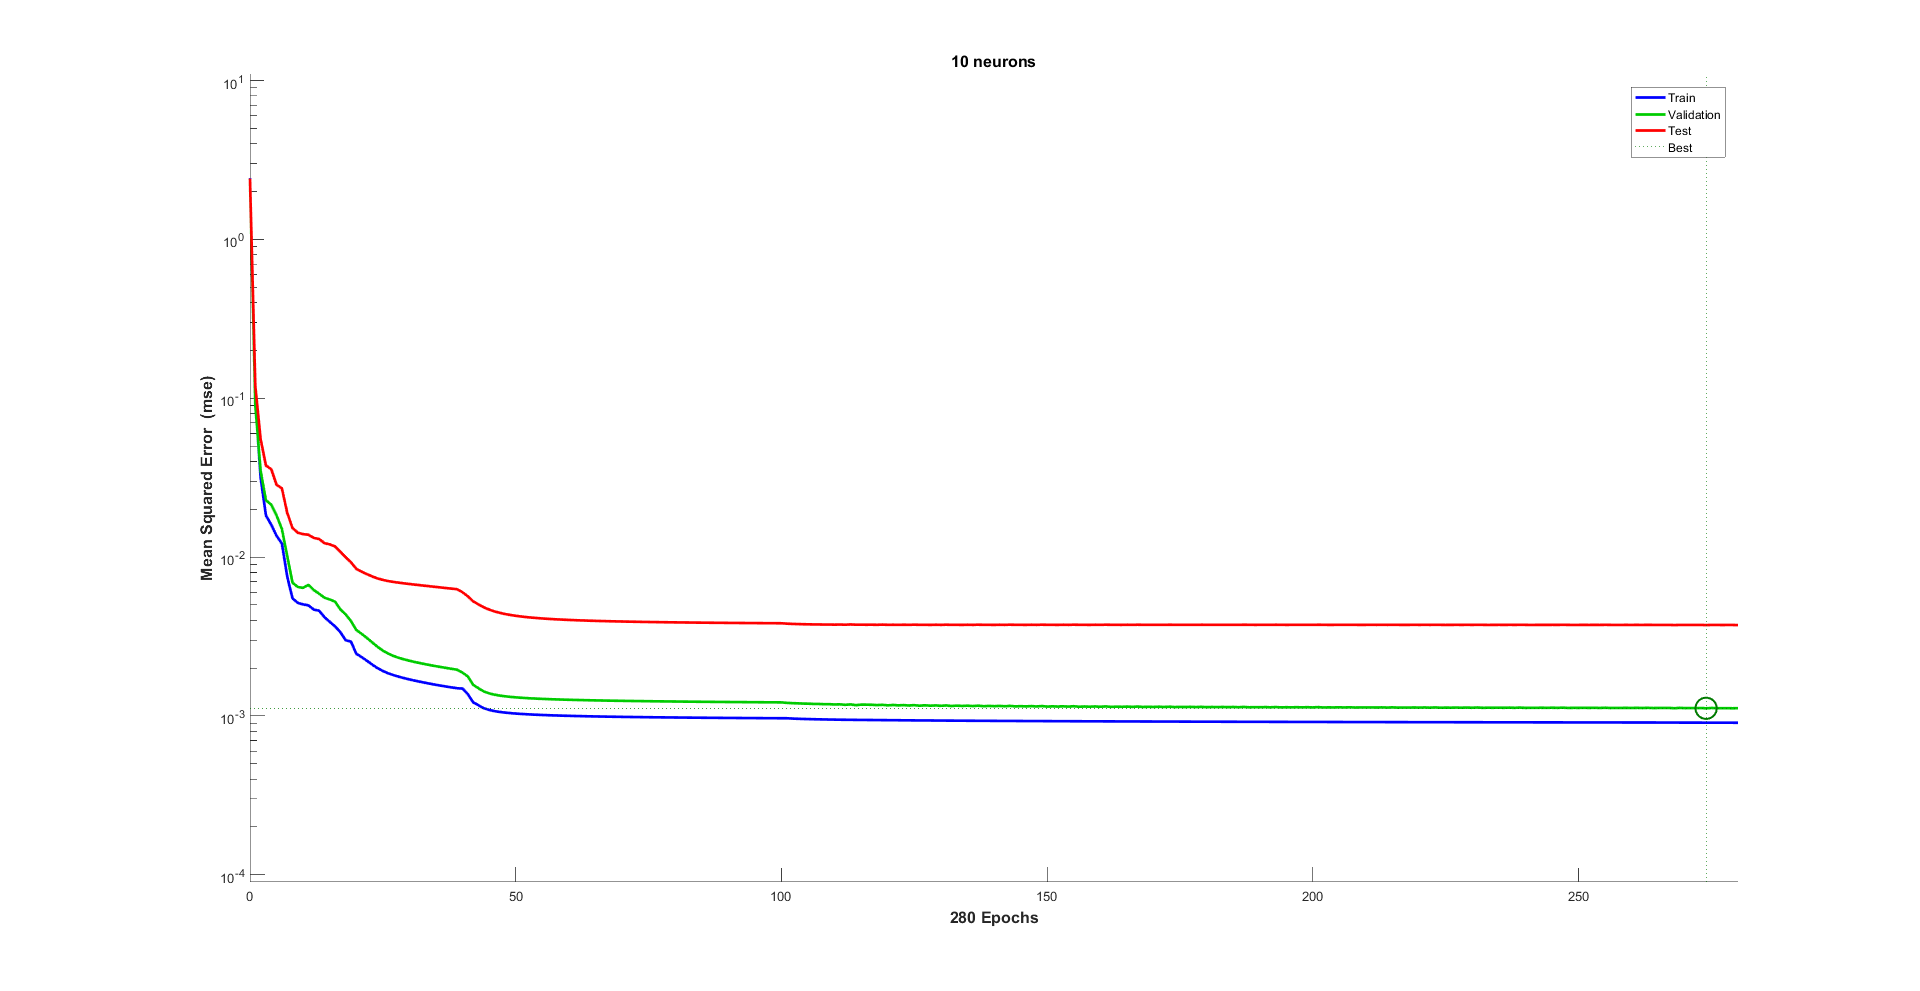
\includegraphics[width=0.45\textwidth]{final/10n}\\
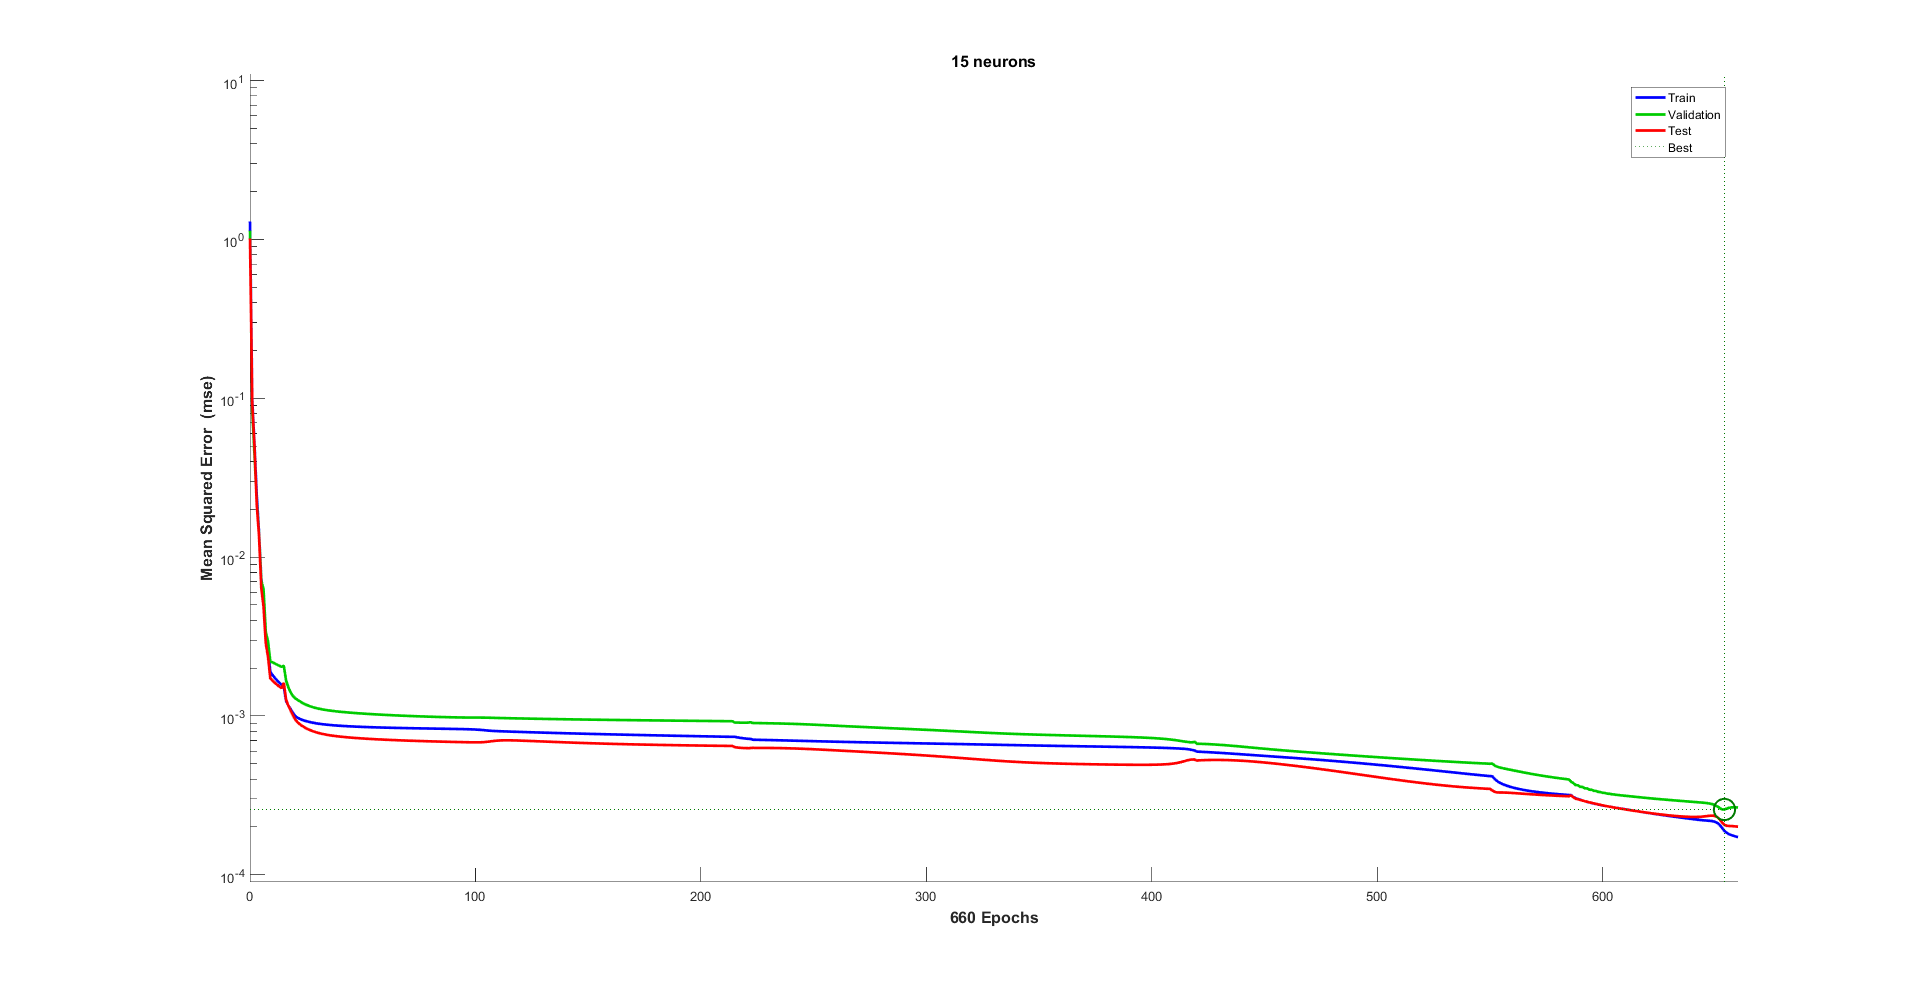
\includegraphics[width=0.45\textwidth]{final/15n} &
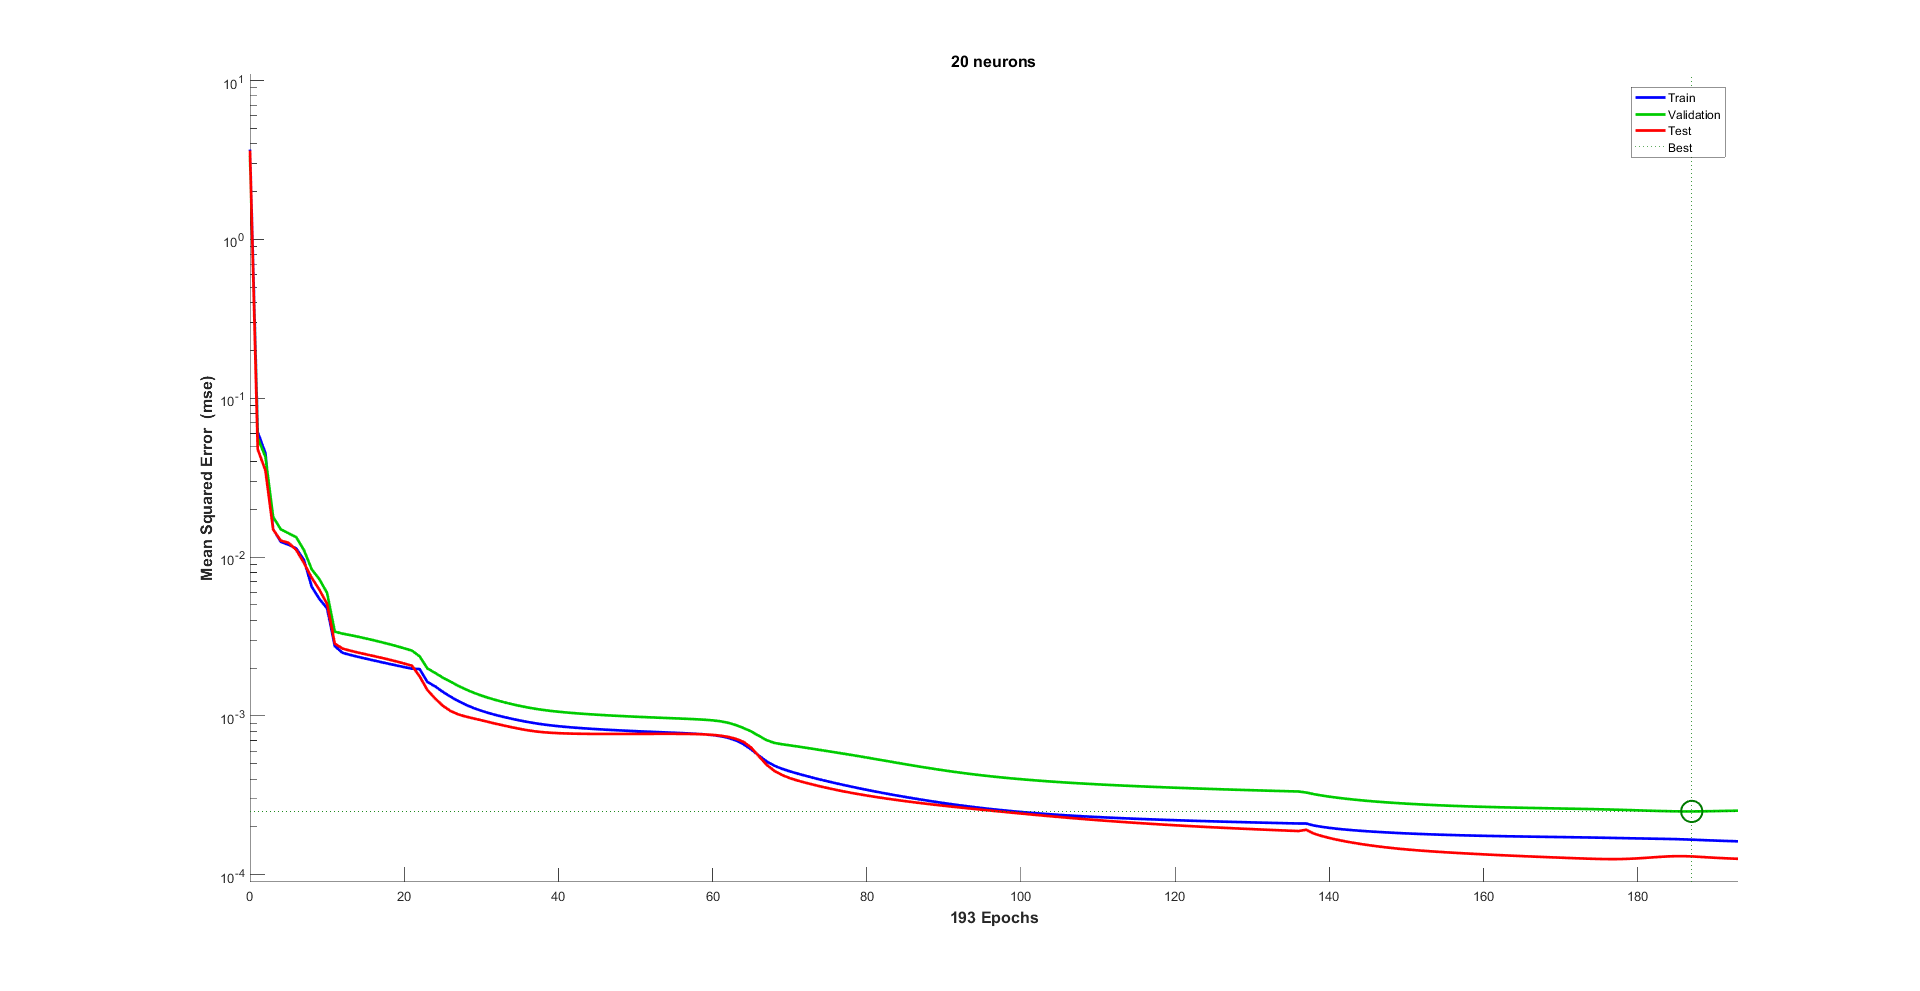
\includegraphics[width=0.45\textwidth]{final/20n} \\
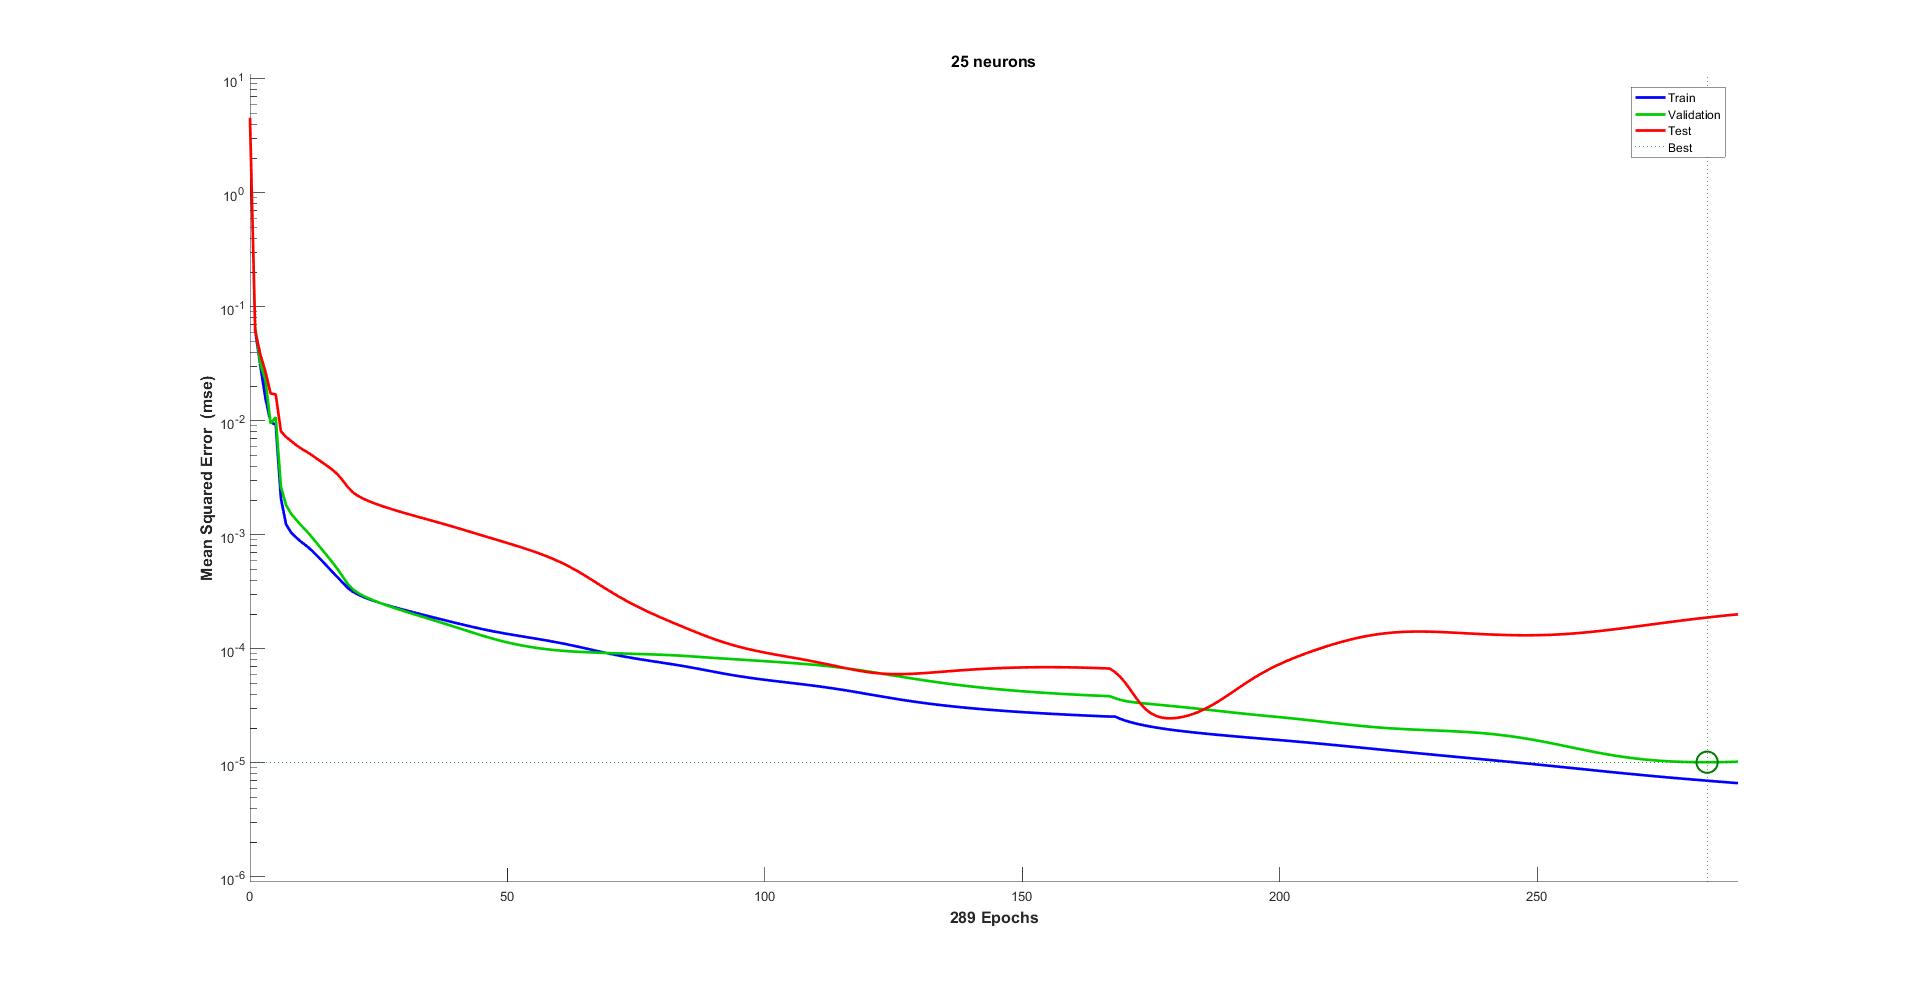
\includegraphics[width=0.45\textwidth]{final/25n} &
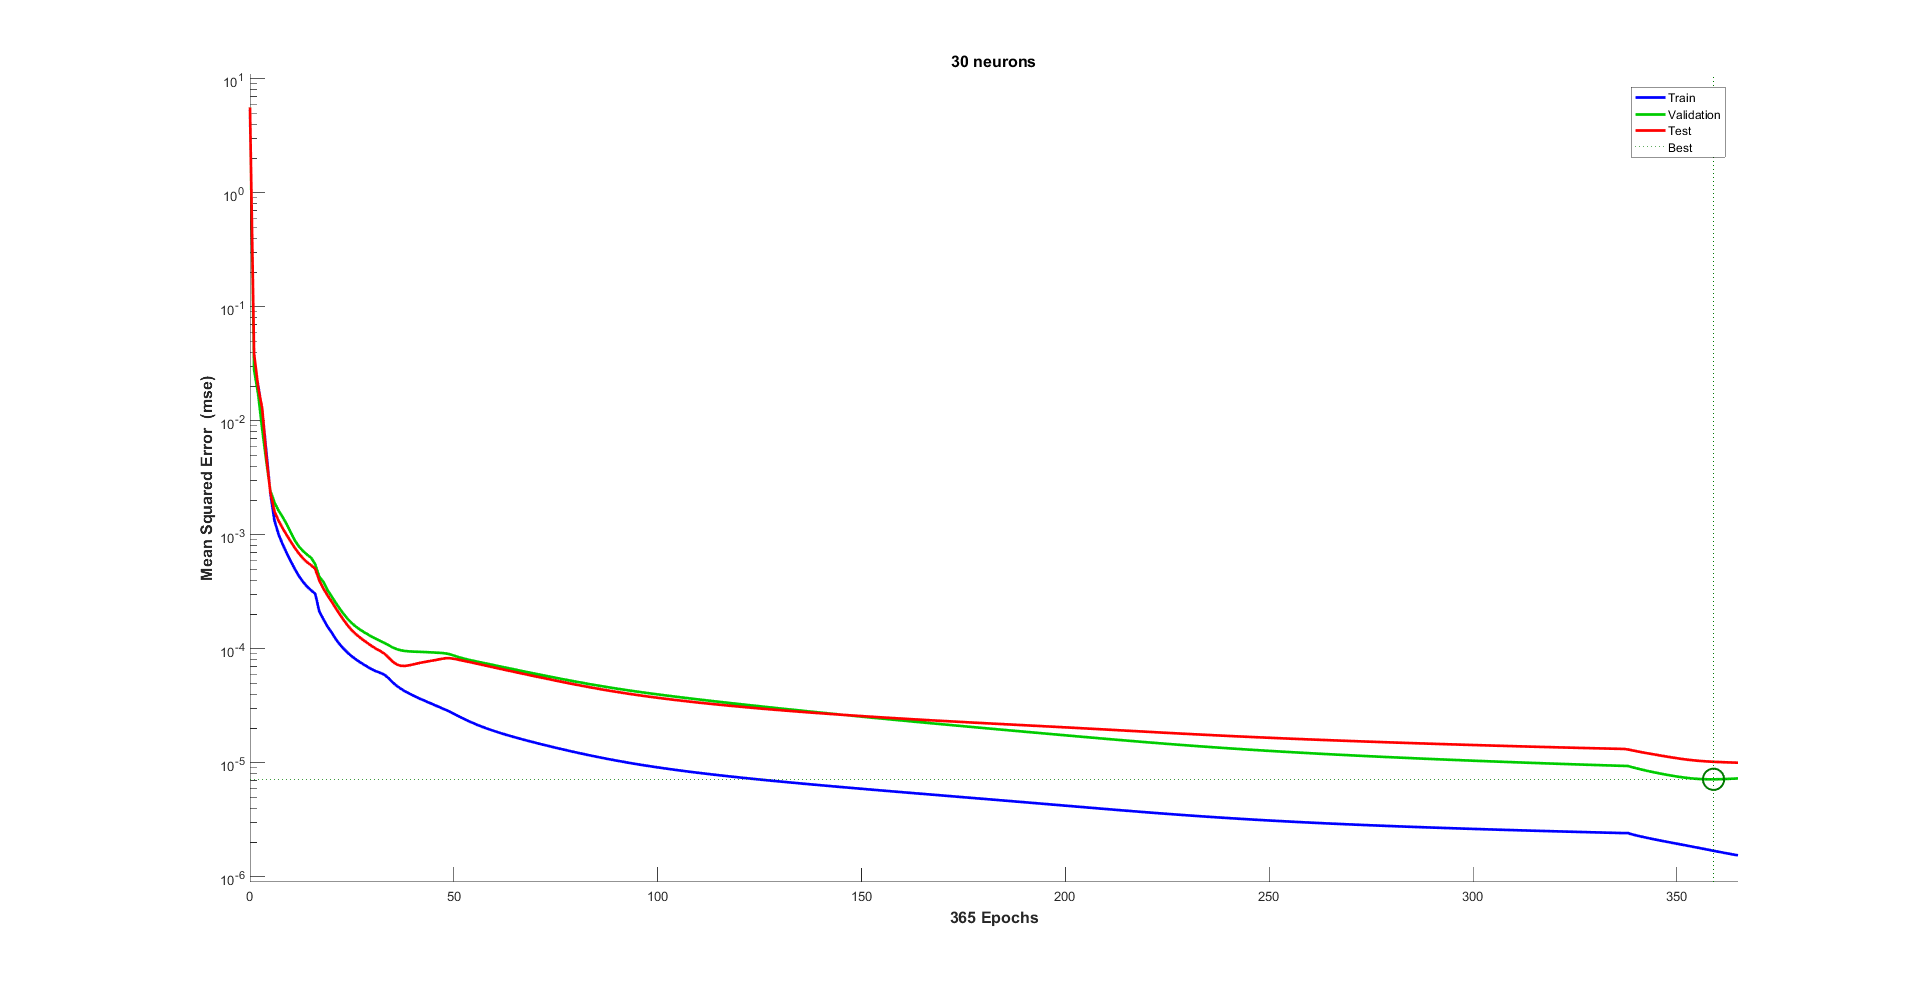
\includegraphics[width=0.45\textwidth]{final/30n}
\end{tabular}
\centering
\end{figure}

\bigbreak
Based on results obtained in sections \textbf{S1} and \textbf{S4}. It was chosen to use a FFNN with one hidden layer, \textit{tansig} and \textit{purelin} as transfer functions and \textit{trainlm} as a learning algorithm. The default parameters according with \cite{matlab_2}. In order to chose a suitable number of neurons in the hidden layer, different networks were tested. According with the results in figure \ref{final_2_2}, the best model was the FFNN with 30 neurons in the hidden layer.
\bigbreak
Finally the performance of the chosen model was assessed using the test set. A total of 100 iterations using different random seeds were run in order to avoid naive results. The MSE average of the model was 1.1736e-05. Figure \ref{final_2_3} shows the result of one of the iterations, in this case the MSE was 1.6656e-06.

\begin{figure}[!htbp]
\caption{Plots of the ground truth and prediction surface. Top: three dimensional view. Middle: two dimensional viewed from the top. Bottom: two dimensional viewed from the bottom.}
\label{final_2_3}
\begin{tabular}{ccc}
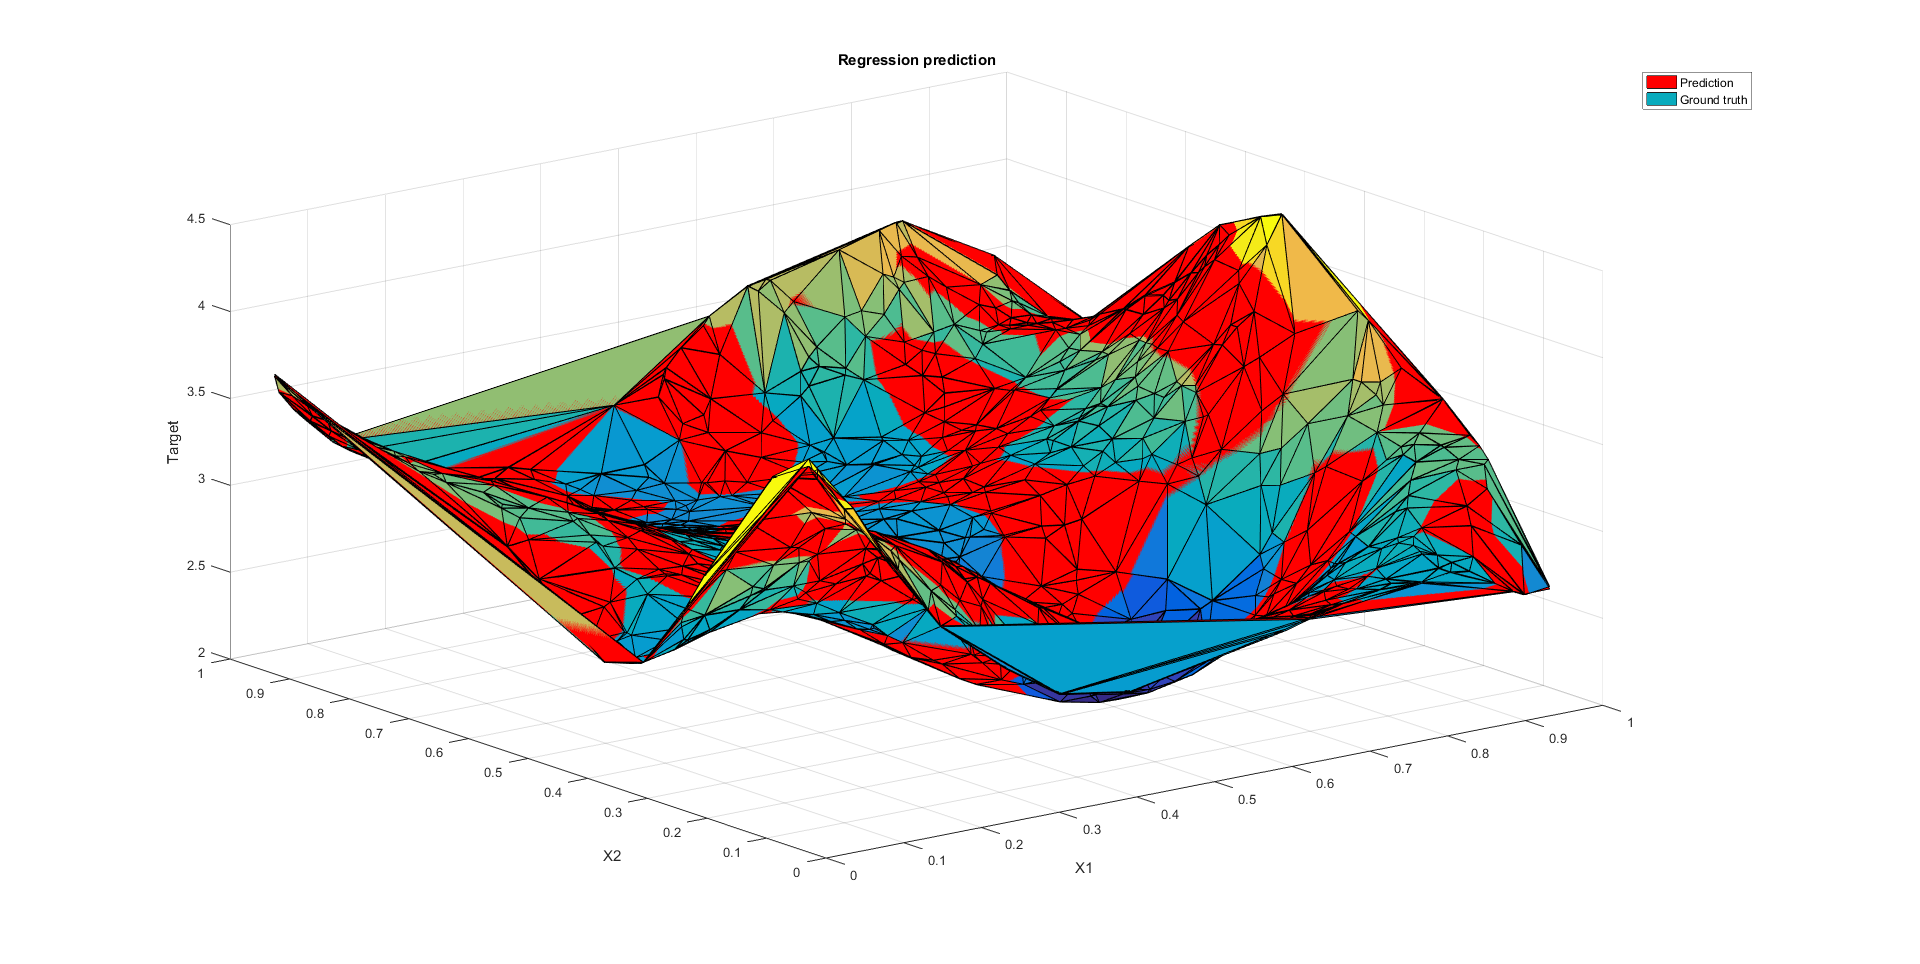
\includegraphics[width=0.9\textwidth]{final/test_prediction_surface1} \\
\includegraphics[width=0.9\textwidth]{final/test_prediction_surface2} \\
\includegraphics[width=0.9\textwidth]{final/test_prediction_surface3}
\end{tabular}
\centering
\end{figure}

\subsection{P1.2: Classification}
The same FFNN architecture, as previous section, was used. Different number of neurons were test in order to set best. Figure \ref{final_3__01} shows the results of the test. According with the results and in contrast with the previous section, the best number of neurons for this specific tasks was 45.
\bigbreak
\begin{figure}[!htbp]
\caption{Results of the classification tasks using different number of neurons}
\label{final_3__01}
\medbreak
\includegraphics[width=0.9\textwidth]{final/preset_fnn_no_dimensionality_reduction}
\centering
\end{figure}

The PCA algorithm was implemented using the code of section \textbf{S3}. Different k componentes were test. Using the knowledge obtained from the experiments of section \textbf{S3} and the results of figure \ref{final_3_2fff}, it was deduced that the best k was 3. In figure \ref{final_3_2fff}, one can see that there is a decay of the cumulative largest values after the third component, which state that after it, there error of the reconstruction will not be reduced dramatically.
\bigbreak
\begin{figure}[!htbp]
\caption{Results of the classification tasks using different number of neurons}
\label{final_3_2fff}
\medbreak
\includegraphics[width=0.9\textwidth]{final/comulative_eigenvalues}
\centering
\end{figure}

A final experiment was assessed, now using the lower dimension data set. In order to have big picture of the different k values and different FFNN models, all the combinations were run. Figure \ref{final_3_3} shows the results. It was noticed that k=3, although it was showed as a good value for PCA, was not necessary the best value. k between 5 and 6 performs better, depending on the number of neurons in the hidden layer.
\bigbreak
\begin{figure}[!htbp]
\caption{Results of the classification tasks using different number of neurons}
\label{final_3_3}
\medbreak
\includegraphics[width=\textwidth]{final/preset_fnn_reduction}
\centering
\end{figure}

Additionally, the overall performance is lower, which indicates that the dataset is sensible to dimensionality reduction. It is reasonable since the dimension is not as big as the dimension of the data set used in section \textbf{S3}. Besides, the the dataset might be high correlated which decreased the performance of the PCA algorithm which can imply a reduction of the performance of the FFNN. It is concluded that inputs are as important as the model of the neural networks; the better the quality of the inputs (features) are, the better the performance of the neural network is. 
\bigbreak
\subsection{P2: Character recognition with Hopfield networks}
As warm-up task, the required letters were created and added to the vocabulary. Figure \ref{all_letter} shows the final results.

\begin{figure}[!htbp]
\caption{Set of letter in the dataset (attractors)}
\label{all_letter}
\includegraphics[width=\textwidth/2]{final/all_letters}
\centering
\end{figure}

In order to tested the accuracy of the Hopfield network, 10,000 iterations were tested using different distorted patterns. Figure \ref{final_3_1} shows the results of one of the iterations. This Hopfield network could recall perfectly the numbers, a MSE average of 0 was obtained. After an exhaustive set of tests, no spurious patterns were found. 
\bigbreak
\begin{figure}[!htbp]
\caption{Top: original letter (attractor state). Middle: distorted letter by 3 pixeles. Bottom: reconstruction using the Hopfield network.}
\label{final_3_1}
\includegraphics[width=\textwidth/2]{final/tasks_2}
\centering
\end{figure}

After the initial experiment, different values of P were tested with 100 epochs. The results of the experiments are shown in figure \ref{spurious_error_state}. This experiments show that the maximum capacity of attractors to generated a perfect recall is roughly 5. This empirical results shown that the theoretical loading capacity using the Hebb-rule (figure \ref{teoretical_hebb}) can be a little off with the actual capacity. However it is a good estimation in order to prevent unexpected states (spurious patterns).
\bigbreak

\begin{figure}[!htbp]
\caption{Average of absolute error and number of spurious patterns found with different P values.}
\label{spurious_error_state}
\includegraphics[width=0.8\textwidth]{final/spurious_error_state}
\centering
\end{figure}

\begin{figure}[!htbp]
\caption{Theoretical loading capacity using the Hebb-rule.}
\label{teoretical_hebb}
\medbreak
\includegraphics[width=0.9\textwidth]{final/teoretical_hebb}
\centering
\end{figure}

An alternative to overcome this downside of the Hopfield network can be a simple, yet powerful, FFNN. In fact, a FFNN was implemented with one hidden layer  using the default settings and 10 neurons in the hidden layer and 35 neurons in the output layer. A dataset of 1,000 samples was created. 80\% of samples were used as training test and validation test and the rest was used as test set. The overall CCR of the FFNN was 96.71\%. Figure \ref{neural_network_35_ouputs} shows the results of the first 5 predictions.

\begin{figure}[!htbp]
\caption{Top: Original letter. Middle: distorted letter by 3 pixeles. Bottom: prediction of the FFNN.}
\label{neural_network_35_ouputs}
\includegraphics[width=0.5\textwidth]{final/neural_network_35_ouputs}
\centering
\end{figure}




\newpage
\appendix
\section{Code: Nonlinear regression}
\begin{lstlisting}[frame=single]
clear;
clc;
close all;

load('Data_Problem1_regression.mat')

%student number r0605947

% *********************** Preprocessing ***********************

Tnew = (9*T1 + 7*T2 + 6*T3 + 5*T4 + 4*T5) / (9+7+6+5+4);
Inputs = [X1 X2];

% *********************** Task 1 ***********************
% Get independent samples
rng(97654); %Use to have the same indices to compare results 
Indices = randperm(size(Tnew,1)); 

Itraning = Indices(1:1000);
Ivalidation = Indices(1001:2000);
Itest = Indices(2001:3000);

Xtraning = Inputs(Indices(1:1000),:);
Tvalidation = Tnew(Indices(1:1000),:);

Xtest = Inputs(Indices(1001:2000),:);
Ttest = Tnew(Indices(1001:2000),:);

% Plot the surface of training set
figure;
plot(Xtraning(:,1),Xtraning(:,2),'o');
title('Training set surface');
xlabel('X1');
ylabel('X2');

% *********************** Task 2 ***********************

max_epochs = 1000;

% creation of networks - 5 neurons
net5=feedforwardnet(5,'trainlm');
% training
net5.trainParam.epochs=max_epochs;
[net5,tr5]=train(net5,Xtraning',Tvalidation');

%creation of networks - 10 neurons
net10=feedforwardnet(10,'trainlm');
%training
net10.trainParam.epochs=max_epochs;
[net10,tr10]=train(net10,Xtraning',Tvalidation');

%creation of networks - 15 neurons
net15=feedforwardnet(15,'trainlm');
%training
net15.trainParam.epochs=max_epochs;
[net15,tr15]=train(net15,Xtraning',Tvalidation');

%creation of networks - 20 neurons
net20=feedforwardnet(20,'trainlm');
%training
net20.trainParam.epochs=max_epochs;
[net20,tr20]=train(net20,Xtraning',Tvalidation');

%creation of networks - 25 neurons
net25=feedforwardnet(25,'trainlm');
%training
net25.trainParam.epochs=max_epochs;
[net25,tr25]=train(net25,Xtraning',Tvalidation');

%creation of networks - 30 neurons
net30=feedforwardnet(30,'trainlm');
%training
net30.trainParam.epochs=max_epochs;
[net30,tr30]=train(net30,Xtraning',Tvalidation');

figure;
plotperform(tr5);
title('5 neurons');
figure;
plotperform(tr10);
title('10 neurons');
figure;
plotperform(tr15);
title('15 neurons');
figure;
plotperform(tr20);
title('20 neurons');
figure;
plotperform(tr25);
title('25 neurons');
figure;
plotperform(tr30);
title('30 neurons');


% *********************** Task 3 ***********************

net=feedforwardnet(30,'trainlm');
%training
net.trainParam.epochs=350;
net=train(net,Xtraning',Tvalidation');

Y_eval_tr = net(Xtest');
Y_eval = Y_eval_tr';

figure;
tri = delaunay(Xtest(:,1),Xtest(:,2));
trisurf(tri,Xtest(:,1),Xtest(:,2), Y_eval)
hold on
tri = delaunay(Xtest(:,1),Xtest(:,2));
trisurf(tri,Xtest(:,1),Xtest(:,2), Ttest)
title('Regression prediction');
xlabel('X1');
ylabel('X2');
zlabel('Target');
hold off

err = immse(Ttest, Y_eval);
fprintf('\n The mean-squared error is %0.4f\n', err);

iterations = 100;
err_m = (iterations);

for i = 1:iterations
    rng(i); % change seed for each iteration
    Indices = randperm(size(Tnew,1)); 

    Itraning = Indices(1:1000);
    Ivalidation = Indices(1001:2000);
    Itest = Indices(2001:3000);

    Xtraning = Inputs(Indices(1:1000),:);
    Tvalidation = Tnew(Indices(1:1000),:);

    Xtest = Inputs(Indices(1001:2000),:);
    Ttest = Tnew(Indices(1001:2000),:);


    net=feedforwardnet(30,'trainlm');
    %training
    net.trainParam.epochs=350;
    net=train(net,Xtraning',Tvalidation');

    Y_eval_tr = net(Xtest');
    Y_eval = Y_eval_tr';

    err_m(i) = immse(Ttest, Y_eval);
end

avg_error = mean(err_m);
fprintf('\n The average mean-squared error is %0.4f using %d iterations\n', avg_error, iterations);

figure;
plot(err_m);
\end{lstlisting}
\section{Code: Classification}
\begin{lstlisting}[frame=single]
clear;
clc;
close all;

% **************** Preprocessing data ****************
rng(97654); %Use to have the same indices to compare results
% Load data
% Positive 4 and 5
% Negative 6

all_raw_set = importdata('winequality-red.csv',';');
all_set = all_raw_set.data;
positive_samples_4 = all_set(all_set(:,end) == 4, :);
positive_samples_5 = all_set(all_set(:,end) == 5, :);
negative_samples = all_set(all_set(:,end) == 6, :);

% Concatenate set as input set 
X = [positive_samples_4(:,1:end-1); 
    positive_samples_5(:,1:end-1);
    negative_samples(:,1:end-1)];

% Convert set into suitable format for output, 1 for 
% positive and -1 for negative class and concatenate them as 
% target set
n_positive = length(positive_samples_4) + length(positive_samples_5);
n_negative = length(negative_samples);
Y = [ones(n_positive,1);
    -ones(n_negative,1)];

% Split data into training set, validation set and test set.
% I used randperm to have an evenly distribution od the 
% samples.
% Total oof samples are 1372 I roughly divided 80% for 
% training set (1000 samples) and 20% for test set
% (372 samples).

n_samples = n_positive + n_negative;
randIdx = randperm(n_samples);

training_set = X(randIdx(1:1000),:);
validation_set = Y(randIdx(1:1000),:);
test_set = X(randIdx(1001:end),:);
ground_truth =  Y(randIdx(1001:end),:);

% **************** task 1 ****************


% Create network without reduced dimensionality
result_matrix = zeros(50);

for neurons=5:5:50
	net1=feedforwardnet(neurons,'trainlm');

	% Training and simulation
	net1.trainParam.epochs=1000;
	net1=train(net1,training_set',validation_set');

	% Performance on test set
	predictions = net1(test_set');
	ccr1 = (sum(sign(predictions) == ground_truth')*100)/length(ground_truth);
	result_matrix(neurons) = ccr1;
end

result_matrix( ~any(result_matrix,2), : ) = [];
result_matrix( :, ~any(result_matrix,1) ) = [];

figure;
x = 5:5:50;
bar(x,result_matrix);

% **************** task 2 ****************

% Find the k optimal components
conv_x = cov(training_set);
[E,s] = eigs(conv_x);
cumsum_values = diag(cumsum(s,100));

figure;
plot(cumsum_values);
title('Comulative sum of the largest eigenvalues');
xlabel('k component');
ylabel('Comulative eigenvalues');


% Process training and test sets to apply PCA
k = 11;

result_matrix = zeros(50,11);
for neurons=5:5:50
    for k=1:11
        % Apply PCA to training set
        conv_x = cov(training_set);
        [E,s] = eig(conv_x);
        [~, indx] = sort(diag(s), 'descend');
        E =E(:,indx);
        projection_training = E(:,1:k)';
        training_set_reduction = projection_training*training_set';


        % Apply PCA to test set
        conv_x = cov(test_set);
        [E,s] = eig(conv_x);
        [s, indx] = sort(diag(s), 'descend');
        E =E(:,indx);
        projection_test = E(:,1:k)';
        test_set_reduction = projection_test*test_set';


        % **************** task 3 ****************
        % Create network with reduced dimensionality
        net2=feedforwardnet(neurons,'trainlm');

        % Training and simulation
        net2.trainParam.epochs=1000;
        net2=train(net2,training_set_reduction,validation_set');

        % Performance on test set
        predictions = net2(test_set_reduction);
        ccr2 = (sum(sign(predictions) == ground_truth')*100)/length(ground_truth);
        fprintf('neurons=%f k=%f CRR=%f \n',neurons,k, ccr2);
        result_matrix(neurons,k) = ccr2;
    end 
end

result_matrix( ~any(result_matrix,2), : ) = [];

figure;
x = 5:5:50;
bar(x, result_matrix);
\end{lstlisting}
\section{Code: Character recognition with Hopfield networks}
\subsection{Main code}
\begin{lstlisting}[frame=single]
clear;
clc;
close all;

% daniel perez -> danielprz

% **************** Preprocessing data ****************
capitals_letters = prprob;
lowercase_letters = lowercase;

X= [lowercase_letters,capitals_letters];
X(X==0)=-1;

% Print all letters
figure;
for i=1:35
    subplot(5,7,i);
    colormap(gray);
    imagesc(reshape(X(:,i),5,7)',[0,1]);
    axis image;
    set(gca,'xtick',[],'ytick',[]);
end

% **************** task 1 ****************
% Create Hopfield Network
num_characters=5;
T = X(:,1:num_characters);
net = newhop(T);

% Distor characters
err=[];

for lo=1:10000
    new_T = zeros(35, num_characters);
    num_pix=3;

    for i=1:num_characters
        indx = randperm(35);
        new_T(:,i) = T(:,i);
        for j=1:num_pix
            new_T(indx(j),i) = T(indx(j),i) * -1;
        end
    end

    [y,Pf,Af] = sim(net,{num_characters 50},{},new_T);

    prediction = sign(y{end});

    err = [err immse(prediction,T)];
end

mean_error = mean(err);

figure;
for i=1:5
    subplot(3,5,i); 
    colormap(gray);
    imagesc(reshape(T(:,i),5,7)',[0,1]);
    axis image;
    set(gca,'xtick',[],'ytick',[]);
    
    subplot(3,5,i+5);
    colormap(gray);
    imagesc(reshape(new_T(:,i),5,7)',[0,1]);
    axis image;
    set(gca,'xtick',[],'ytick',[]);
    
    subplot(3,5,i+10);
    colormap(gray);
    imagesc(reshape(prediction(:,i),5,7)',[0,1]);
    axis image;
    set(gca,'xtick',[],'ytick',[]);
end

% **************** task 2 ****************
erro_by_p = [];
spurious_by_p = [];
spurious_state = [];
for P=1:35
    % Create Hopfield Network
    T = X(:,1:P);
    net = newhop(T);
    err=[];
    inner_counter = 0;
    for iteration=1:100
        new_T = zeros(35, P);
        num_pix=3;
    
        for i=1:P
            indx = randperm(35);
            new_T(:,i) = T(:,i);
            for j=1:num_pix
                new_T(indx(j),i) = T(indx(j),i) * -1;
            end
        end
    
        [y,Pf,Af] = sim(net,{P 50},{},new_T);
        
        if (y{end} ~= y{end-1})
            fprint('Hopfield network does not converge \n');
            break;
        end
        
        prediction = sign(y{end});
    
        err = [err sum(sum(prediction ~= T))];
        
        for psub = 1:P
            ynext = repmat(prediction(:,psub),1,P);
            if(sum(sum(ynext ~= T)==0)==0)
                fprintf('Found spurious state \n');
                spurious_state = [spurious_state prediction(:,psub)];
                inner_counter = inner_counter + 1;
            end
        end
    end   
    spurious_by_p = [spurious_by_p (inner_counter/100)];
    erro_by_p = [erro_by_p mean(err)];
end

figure;
plot(erro_by_p);
hold on;
plot(spurious_by_p);

figure;
for i=1:10
    subplot(1,10,i);
    colormap(gray);
    imagesc(reshape(spurious_state(:,i),5,7)',[0,1]);
    axis image;
    set(gca,'xtick',[],'ytick',[]);
end

% Theoretical Hebb-rule
figure;
Xs = 1:size(X,2);
sig = sqrt(Xs/size(X,1));
Z = 1./sig;
P_error = normcdf(ones(size(Xs))*Inf) - normcdf(Z);
plot(Xs,P_error);

% **************** task 3 ****************
num_characters=25;
T = X(:,1:num_characters);
Target = 
    [T T T T T T T T T T T T T T T T 
    T T T T T T T T T T T T T T T T T T T T T T T T];

t_length = length(Target);

% Training set
training_set = zeros(35, t_length);
num_pix=3;

for i=1:t_length
    indx = randperm(35);
    training_set(:,i) = Target(:,i);
    for j=1:num_pix
        training_set(indx(j),i) = Target(indx(j),i) * -1;
    end
end

randIdx = randperm(1000);
t_set = training_set(:,randIdx(1:800));
validation_set = Target(:,randIdx(1:800));
test_set = training_set(:,randIdx(801:end));
ground_truth =  Target(:,randIdx(801:end));

net1=feedforwardnet(10,'trainlm');

% Training and simulation
net1.trainParam.epochs=500;
net1=train(net1,t_set,validation_set);

% Performance on test set
predictions = net1(test_set);
predictions = sign(predictions);

ccr1 = (sum(sum(predictions == ground_truth)))/(200*35);

figure;
for i=1:5
    subplot(3,5,i+5);
    colormap(gray);
    imagesc(reshape(test_set(:,i),5,7)',[0,1]);
    axis image;
    set(gca,'xtick',[],'ytick',[]);

    subplot(3,5,i+10);
    colormap(gray);
    imagesc(reshape(predictions(:,i),5,7)',[0,1]);
    axis image;
    set(gca,'xtick',[],'ytick',[]);

    subplot(3,5,i);
    colormap(gray);
    imagesc(reshape(ground_truth(:,i),5,7)',[0,1]);
    axis image;
    set(gca,'xtick',[],'ytick',[]);
end
\end{lstlisting}


\subsection{lowercase.m}
\begin{lstlisting}[frame=single]
function [ out ] = lowercase
%danielprz
letterd =  [0 0 0 0 1 0 0 0 0 1 0 0 0 0 1 0 1 1 1 1 1 0 0 0 1 1 0 0 0 1 0 1 1 1 1 ]';

lettera =  [0 0 0 0 0 0 0 0 0 0 0 0 1 1 0 0 1 0 1 0 1 0 0 1 0 1 0 0 1 0 0 1 1 1 1 ]';

lettern =  [0 0 0 0 0 0 0 0 0 0 1 0 1 1 0 1 1 0 0 1 1 0 0 0 1 1 0 0 0 1 1 0 0 0 1 ]';

letteri =  [0 0 1 0 0 0 0 0 0 0 0 1 1 0 0 0 0 1 0 0 0 0 1 0 0 0 0 1 0 0 0 1 1 1 0 ]';

lettere =  [0 0 0 0 0 0 0 1 0 0 0 1 0 1 0 1 1 1 1 1 1 0 0 0 0 1 0 0 0 0 0 1 1 1 0 ]'; 
        
letterl =  [0 1 1 0 0 0 0 1 0 0 0 0 1 0 0 0 0 1 0 0 0 0 1 0 0 0 0 1 0 0 0 1 1 1 0 ]';

letterp =  [1 1 1 0 0 1 0 0 1 0 1 0 0 1 0 1 1 1 1 0 1 0 0 0 0 1 0 0 0 0 1 0 0 0 0 ]';    
        
letterr =  [0 0 0 0 0 0 0 0 0 0 1 0 1 1 0 1 1 0 0 1 1 0 0 0 0 1 0 0 0 0 1 0 0 0 0 ]';
        
letterz =  [0 0 0 0 0 0 0 0 0 0 1 1 1 1 1 0 0 0 1 0 0 0 1 0 0 0 1 0 0 0 1 1 1 1 1 ]';
        
out = [letterd,lettera,lettern,letteri,lettere,letterl,letterp,letterr,letterz];
end
\end{lstlisting}

\bibliographystyle{siam}
\bibliography{references}

\end{document}
